\documentclass[a4paper,12pt,twoside]{report}
\usepackage[margin=1in,headsep=1cm,footskip=1cm]{geometry}
	\setcounter{tocdepth}{3}
	\setcounter{secnumdepth}{3}
\usepackage[main=english]{babel}
\usepackage[utf8]{inputenc}
\usepackage{fancyhdr}
	\pagestyle{fancy}
	\renewcommand{\chaptermark}[1]{\markboth{\textbf{\chaptername\ \thechapter.\ #1}}{}}
	\renewcommand{\headrulewidth}{0.125mm}
	\setlength{\headheight}{15pt}
	%\renewcommand{\footrulewidth}{0.125mm}
%\usepackage{natbib}
	%\bibliographystyle{chicago}
\usepackage{setspace}
	%\setstretch{1.0} %1.0 or 1.3 or 1.6 or \singlespacing or \onehalfspacing or \doublespacing
	\parindent 1cm
	\parskip 6pt
\usepackage{tikz}
	\usetikzlibrary{arrows,chains,matrix,positioning,scopes}
	\tikzset{>=triangle 45} %latex or latex' or stealth or stealth'
%\usepackage{pgfplots}
%tikzplotlib
\usepackage{pgfplots}
\DeclareUnicodeCharacter{2212}{−}
\usepgfplotslibrary{groupplots,dateplot}
\usetikzlibrary{patterns,shapes.arrows}
\pgfplotsset{compat=newest}
\usepackage{graphics}
	\graphicspath{{figures/}}
\usepackage{amsmath}
\usepackage{adjustbox}
\usepackage{array}
\usepackage{bookmark}
\usepackage{booktabs}
\usepackage[labelfont=bf,center]{caption}
\newcommand{\source}[1]{\caption*{Source: {#1}} }
\usepackage{subcaption}
\usepackage{enumerate}
\usepackage{epstopdf}
\usepackage{float}
\usepackage[bottom]{footmisc}
\usepackage{footnote}
\usepackage{lipsum}
\usepackage{longtable}
\usepackage{threeparttable}
\usepackage{multicol}
\usepackage{multirow}
\usepackage{pdflscape}
\usepackage{rotating}
\usepackage{siunitx}
\usepackage{smartdiagram}
\usepackage{xcolor}
\usepackage{hyperref}
\usepackage{url}
\usepackage{csquotes}
\usepackage[linesnumbered,ruled,vlined]{algorithm2e}
%\usepackage[backend=biber, style=authoryear-icomp]{biblatex}
%\usepackage[backend=biber,style=numeric,autocite=plain,sorting=none]{biblatex}
\usepackage[backend=biber]{biblatex}
\addbibresource{bib_file.bib}
\DeclareUnicodeCharacter{2212}{-}

\begin{document}
\begin{onehalfspace}

	\fancyhf{} % Clears all page headers and footers
	\rhead{\thepage}
	\lhead{\nouppercase{\leftmark}} % Sets the right side header to show the page number

\pdfbookmark[chapter]{Titlepage}{titlepage}
\begin{titlepage}
\pagenumbering{Alph}
\begin{center}

\textsc{\huge Università degli Studi di Trento}\\[-0.375cm] % University name
\rule{0.85\linewidth}{0.125mm}\\[0.25cm]
\textsc{\Large Department of Economics and Management}\\[1.25cm] % University requirement text
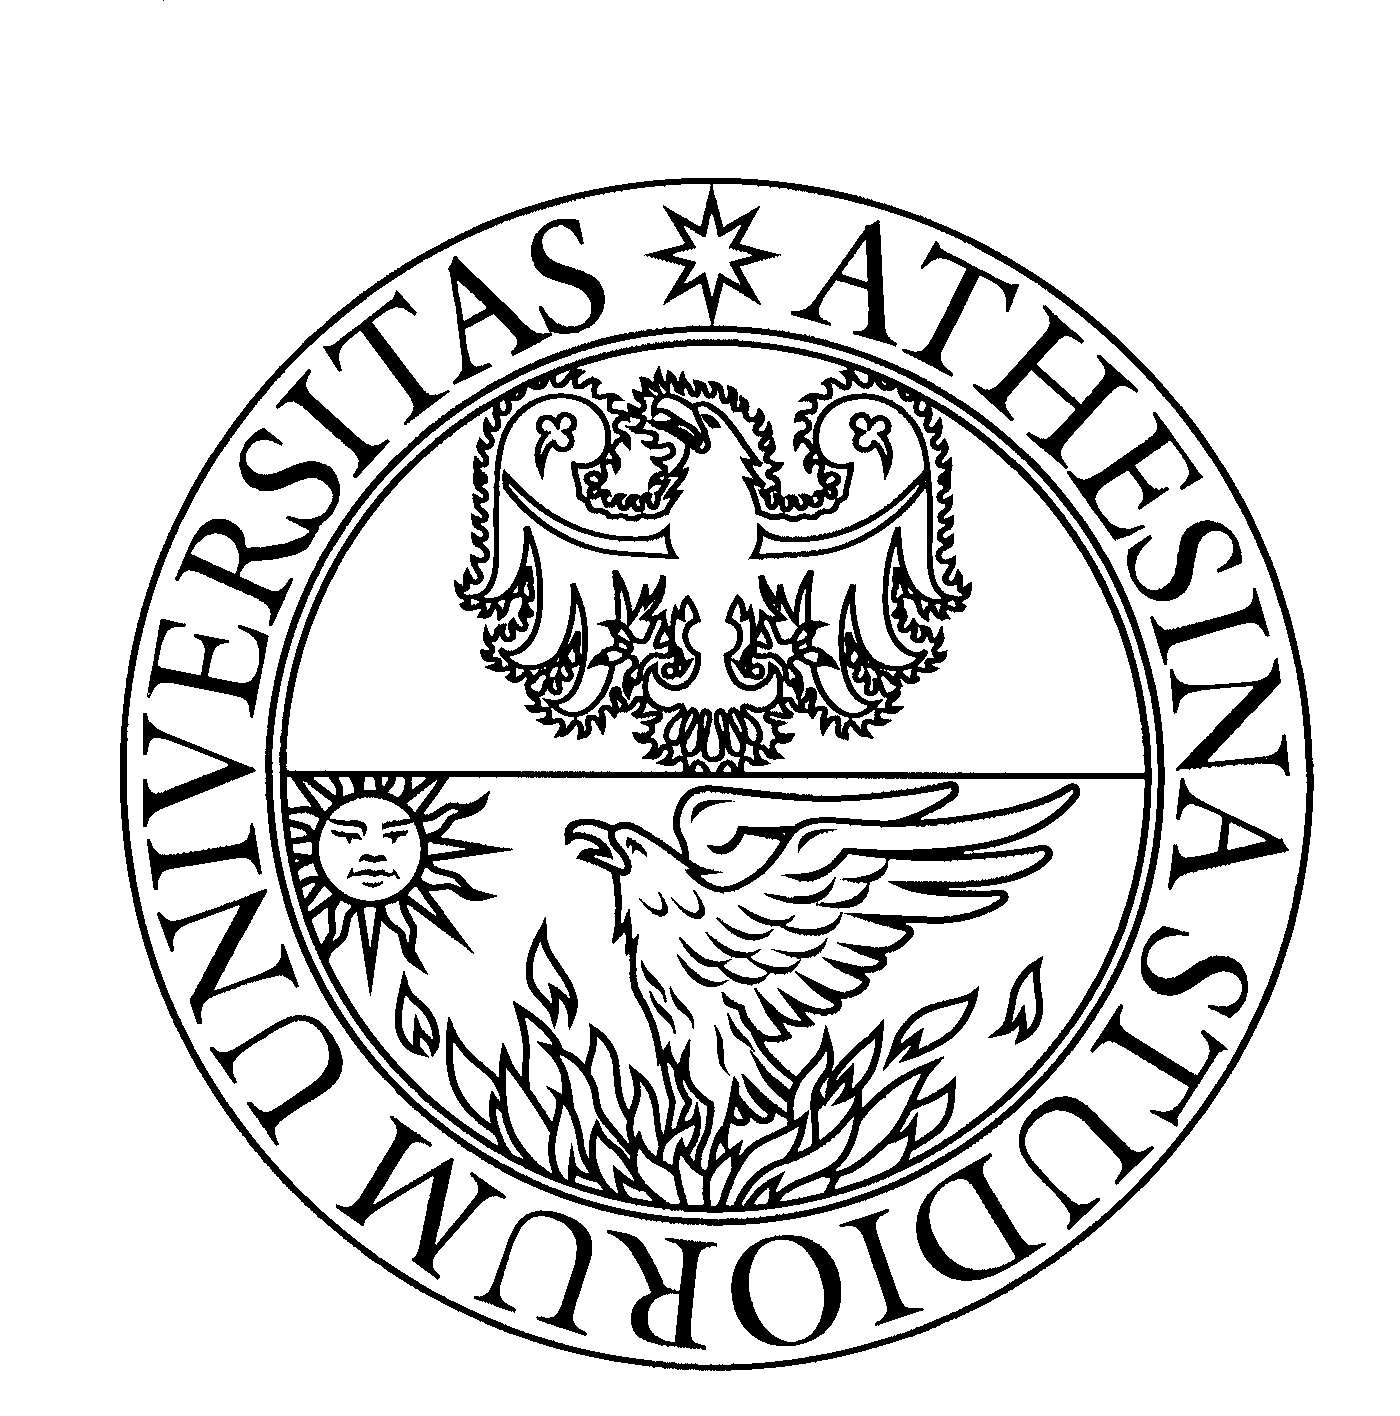
\includegraphics[width=0.3\linewidth]{logo_unitn.png}\\[1.25cm] % University/department logo - uncomment to place it
\textsc{\LARGE Master of Science in Economics}\\[2cm] % University programme
\textsc{\LARGE Master Thesis}\\[0.5cm] % Thesis type

\rule{\linewidth}{0.5mm}\\[0.75cm] % Horizontal line
{\Large \textbf{Using Machine Learning for Airbnb Price Prediction}}\\[0.5cm] % Thesis title
\rule{\linewidth}{0.5mm}\\[1cm] % Horizontal line

\begin{minipage}{0.4\textwidth}
\begin{flushleft} \large
Author:\\
\textsc{Duc Tuong Vu} % Author name - remove the \href bracket to remove the link
\end{flushleft}
\end{minipage}
\begin{minipage}{0.4\textwidth}
\begin{flushright} \large
Supervisor:\\
Prof. \textsc{XXX} % Supervisor name - remove the \href bracket to remove the link
\end{flushright}
\end{minipage}\\[3cm]

\textsc{Academic Year 2020/2021}\\[0.25cm] % University requirement text

\vfill

\end{center}
\end{titlepage}

\clearpage
	\fancyhf{}
	\rhead{\thepage}
	\lhead{\textbf{Acknowledgments}}
\phantomsection
%\pdfbookmark[chapter]{Acknowledgments}{Acknowledgments}
\addcontentsline{toc}{chapter}{Acknowledgments}
\pagenumbering{roman}
\chapter*{Acknowledgments}
\label{c:ack}
I would first like to pay special regards to my thesis advisor Professor. Marco
Bee of the Department of Economics and Management at the University of Trento.
The door to Professor Bee's office was always open whenever I ran into a
trouble spot or had a question about my research or writing. He consistently
allowed this paper to be my work but steered me in the right direction
whenever he thought I needed it.

Some special words of gratitude go to my friends who have always been a
significant source of support when things get a bit discouraging: Federico,
Nick, Ivan, Thai, Giang, Thuy, Hong. Thank you guys for always be there for me.

Nobody has more important to me in the pursuit of this project than the members
of my family. I would like to thank my parents for their great love and
understanding. To my brother Lieu, you are always in my heart, and  I hope you
get well soon. Most importantly, I wish to thank my brother Ly for providing me with
unfailing support and continuous encouragement throughout my years of study and
through the process of researching and writing this thesis.





\clearpage
	\fancyhf{}
	\rhead{\thepage}
	\lhead{\textbf{ \nouppercase{\leftmark}} }
\phantomsection
%\pdfbookmark{\contentsname}{toc}
\addcontentsline{toc}{chapter}{Contents}
\tableofcontents

\clearpage
\phantomsection
%\pdfbookmark[chapter]{List of Figures}{lof}
\addcontentsline{toc}{chapter}{List of figures}
\listoffigures

\clearpage
\phantomsection
%\pdfbookmark[chapter]{List of Tables}{lot}
\addcontentsline{toc}{chapter}{List of tables}
\listoftables

\clearpage
	\fancyhf{}
	\rhead{\thepage}
	\lhead{\textbf{Abstract}}
\phantomsection
%\pdfbookmark[chapter]{Abstract}{Abstract}
\addcontentsline{toc}{chapter}{Abstract}
\chapter*{Abstract}
\label{c:abstract}

Lorem ipsum dolor sit amet, consetetur sadipscing elitr, sed diam nonumy eirmod tempor invidunt ut labore et dolore magna aliquyam erat, sed diam voluptua. At vero eos et accusam et justo duo dolores et ea rebum. Stet clita kasd gubergren, no sea takimata sanctus est Lorem ipsum dolor sit amet.

\textbf{Keywords:}



\clearpage
	\fancyhf{}
	\rhead{\thepage}
	\lhead{\nouppercase{\leftmark}}
\pagenumbering{arabic}
\chapter{Introduction}
\label{c:intro}
Pricing a rental property on Airbnb is a challenging task for the owner as it
determines the number of customers for the place

\section{Motivation and Goals}
\label{sect_intro_motivation}

In recent years


\section{Literature Review}
\label{sect_intro_literature_review}

Parts of the existing literature on property pricing focus on non-shared
property purchase or rental price prediction





\clearpage
\chapter{Data Set}
\label{c:dataset}



Lorem ipsum dolor sit amet, consetetur sadipscing elitr, sed diam nonumy eirmod tempor invidunt ut labore et dolore magna aliquyam erat, sed diam voluptua. At vero eos et accusam et justo duo dolores et ea rebum. Stet clita kasd gubergren, no sea takimata sanctus est Lorem ipsum dolor sit amet.


\section{Data Acquisition}
\label{sec:data_acquisition}

Lorem ipsum dolor sit amet, consetetur sadipscing elitr, sed diam nonumy eirmod tempor invidunt ut labore et dolore magna aliquyam erat, sed diam voluptua. At vero eos et accusam et justo duo dolores et ea rebum. Stet clita kasd gubergren, no sea takimata sanctus est Lorem ipsum dolor sit amet.


\section{Data Cleaning }
\label{sec:data_cleaning}

Lorem ipsum dolor sit amet, consetetur sadipscing elitr, sed diam nonumy eirmod tempor invidunt ut labore et dolore magna aliquyam erat, sed diam voluptua. At vero eos et accusam et justo duo dolores et ea rebum. Stet clita kasd gubergren, no sea takimata sanctus est Lorem ipsum dolor sit amet.

\subsection{Incomplete, Missing Data}

Lorem ipsum dolor sit amet, consetetur sadipscing elitr, sed diam nonumy eirmod tempor invidunt ut labore et dolore magna aliquyam erat, sed diam voluptua. At vero eos et accusam et justo duo dolores et ea rebum. Stet clita kasd gubergren, no sea takimata sanctus est Lorem ipsum dolor sit amet.

\subsection{Variable Selection and Filtering}

Lorem ipsum dolor sit amet, consetetur sadipscing elitr, sed diam nonumy eirmod tempor invidunt ut labore et dolore magna aliquyam erat, sed diam voluptua. At vero eos et accusam et justo duo dolores et ea rebum. Stet clita kasd gubergren, no sea takimata sanctus est Lorem ipsum dolor sit amet.


\section{Exploratory Data Analysis}
\label{sec:eda}

Lorem ipsum dolor sit amet, consetetur sadipscing elitr, sed diam nonumy eirmod tempor invidunt ut labore et dolore magna aliquyam erat, sed diam voluptua. At vero eos et accusam et justo duo dolores et ea rebum. Stet clita kasd gubergren, no sea takimata sanctus est Lorem ipsum dolor sit amet.



\clearpage
\chapter{Exploratory Data Analysis}
\label{c:eda}

Before embarking on developing statistical models and generating predictions, it
is essential to understand your data. This is typically done using conventional
numerical and graphical methods. \textcite{tukey1977exploratory} advocated the practice
of exploratory data analysis (EDA) as a critical part of the scientific process.


We present the descriptive statistics of variables in Table
\ref{tab:descriptive-statistic}


\section{Numerical Features}
\label{sec:numerical_features}


\subsection{Price}

The nightly advertised prices range from \$0 to \$10,000. The range is so broad
because hosts do not understand how to set Airbnb advertised prices.  Figure
~\ref{fig:price-distribution-1000} and Figure ~\ref{fig:price-distribution-200}
 show the distributions of price up to \$1,000 and \$200 respectively. While the
price's range is extensive, most of its values concentrate on the range \$10 to
\$1000.  Hence, for minimal values under \$10, we will increase them to \$10,
and values above \$1,000 will be reduced to \$1,000.
\begin{figure}[H]
    %\centering
    \begin{center}

    \caption{Price Distribution}
    \begin{subfigure}[b]{0.48\textwidth}
        \centering
        \caption{Airbnb advertised price up to \$1000}
        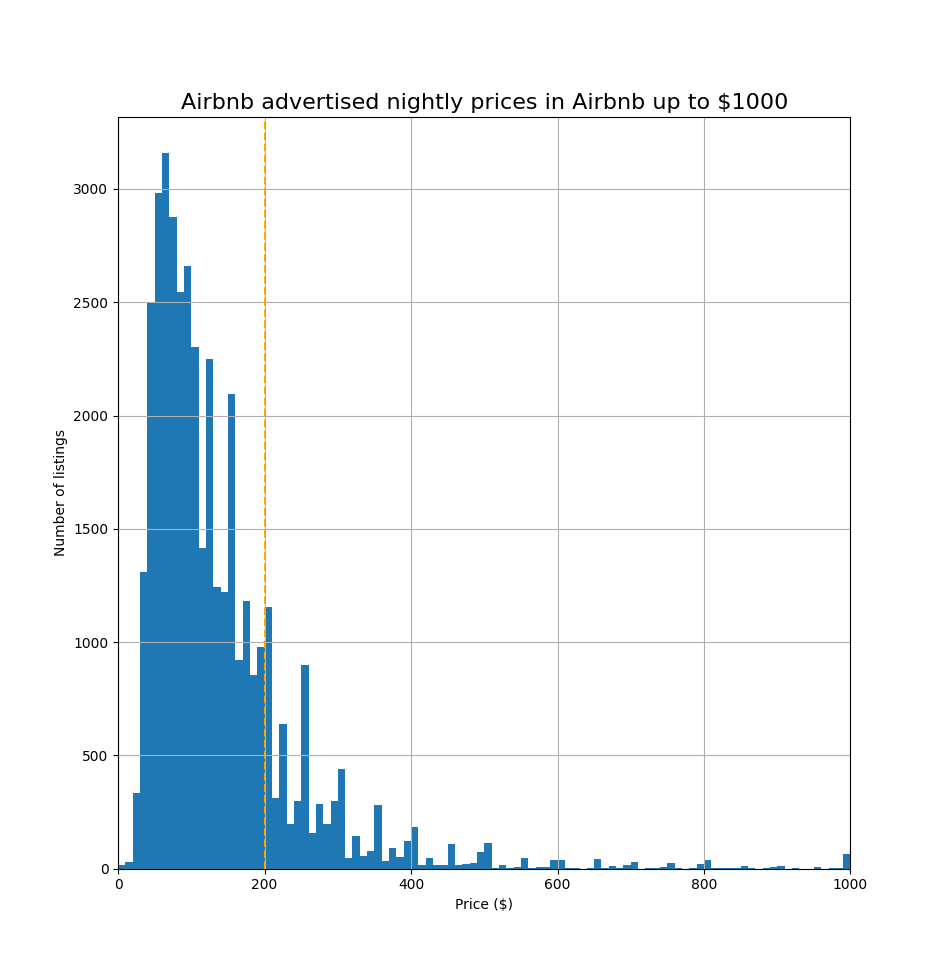
\includegraphics[width=\textwidth]{Figure_6.png}
        \label{fig:price-distribution-1000}
    \end{subfigure}
    \begin{subfigure}[b]{0.48\textwidth}
        \centering
        \caption{Airbnb advertised price up to \$200}
        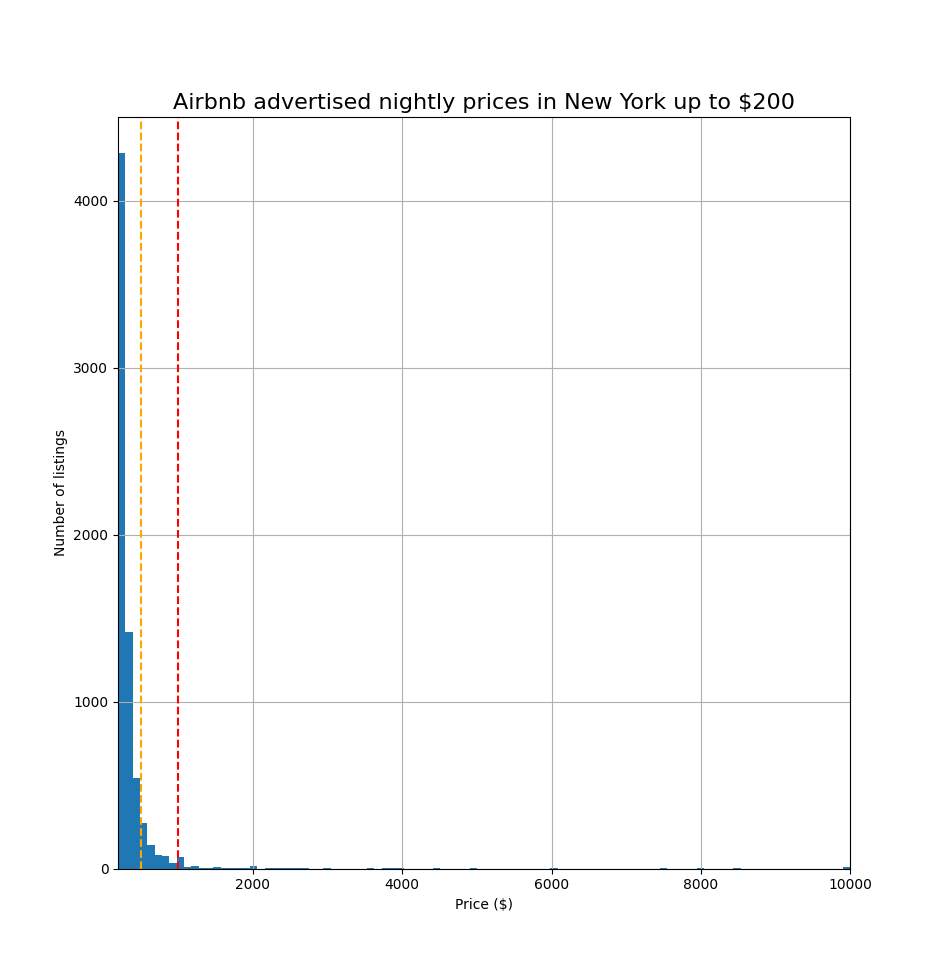
\includegraphics[width=\textwidth]{Figure_7.png}
        \label{fig:price-distribution-200}
    \end{subfigure}

    \end{center}
\end{figure}

\subsection{Host Listings Count}

The median number of listings that the host of each listing has is 1. The mean
is higher (8 in total) due to some hosts own many listings. About 55\% of
listings are from hosts with one listing, and 45\% are from multi-listing hosts.

\subsection{Number of people accommodated, bathrooms, bedrooms and beds}

Figure ~\ref{fig:hist-accommodates} reveals that the most common listing type accommodates two people in
one bed in one bedroom with one bathroom.

\begin{figure}[H] \centering
\caption{Histogram Plot of Accomodate, Bathrooms, Bedrooms, and Beds}
    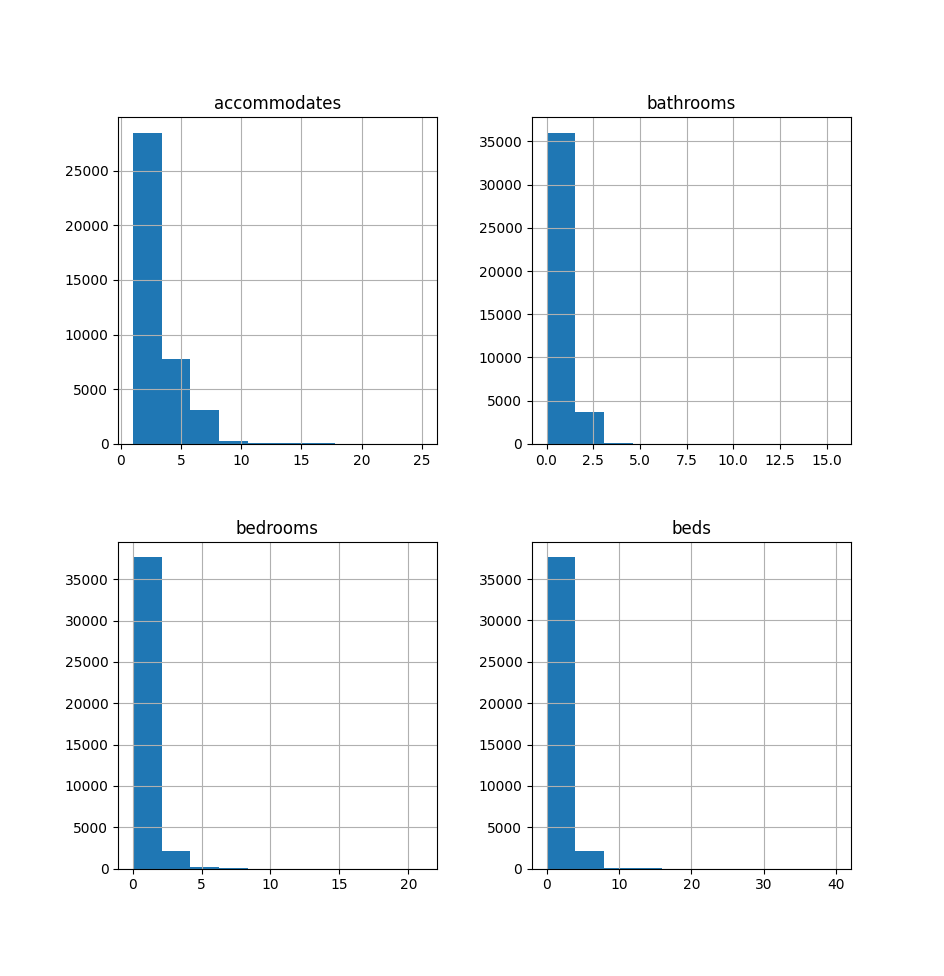
\includegraphics[width=0.75\textwidth]{Figure_9.png}
    \label{fig:hist-accommodates}
\end{figure}

Figure ~\ref{fig:median-price-accommodates} shows that the more people a listing accommodates, the higher the
price they can charge their customers.

\begin{figure}[H] \centering
\caption{Median Price of Airbnb Listing Accommodating Different Number Of Guests}
    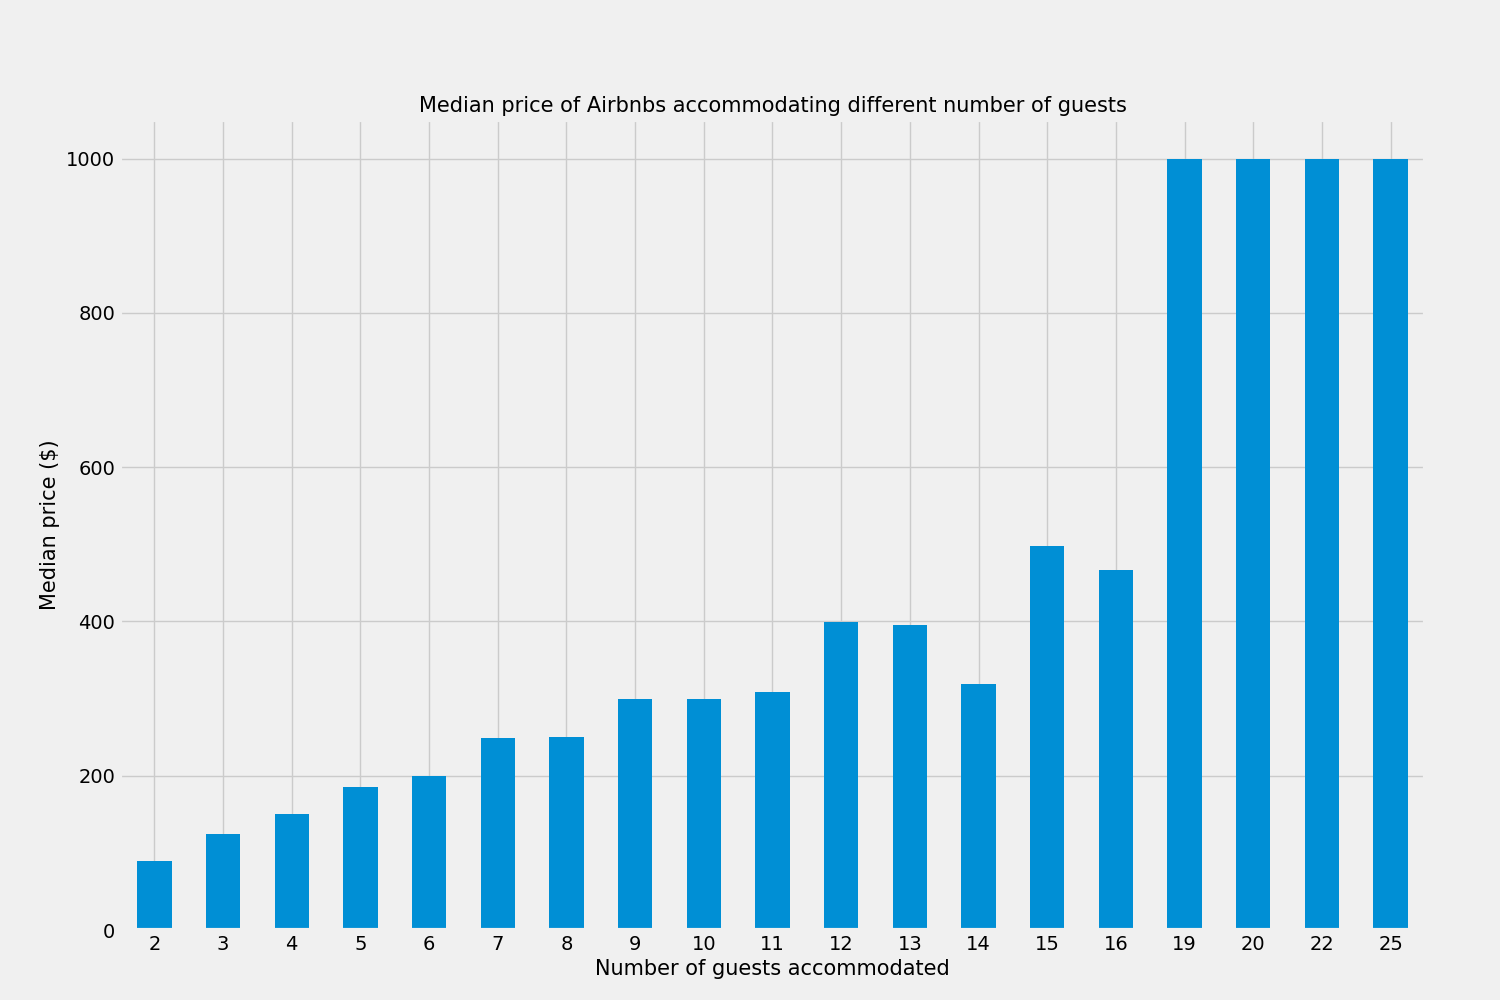
\includegraphics[width=0.75\textwidth]{Figure_8.png}
    \label{fig:median-price-accommodates}
\end{figure}

\section{Categorical features}
\label{sec:categorical_features}

Our main EDA objective for categorical data is to know the unique values and
their corresponding count.

\subsection{Neighbourhood}

Manhattan and Brooklyn have the most Airbnb properties, followed by
Queens (Figure \ref{fig:borough-number-of-listing})
%\begin{figure}[h]\centering
    %\caption{Number of Airbnb listings in each New York borough}
    %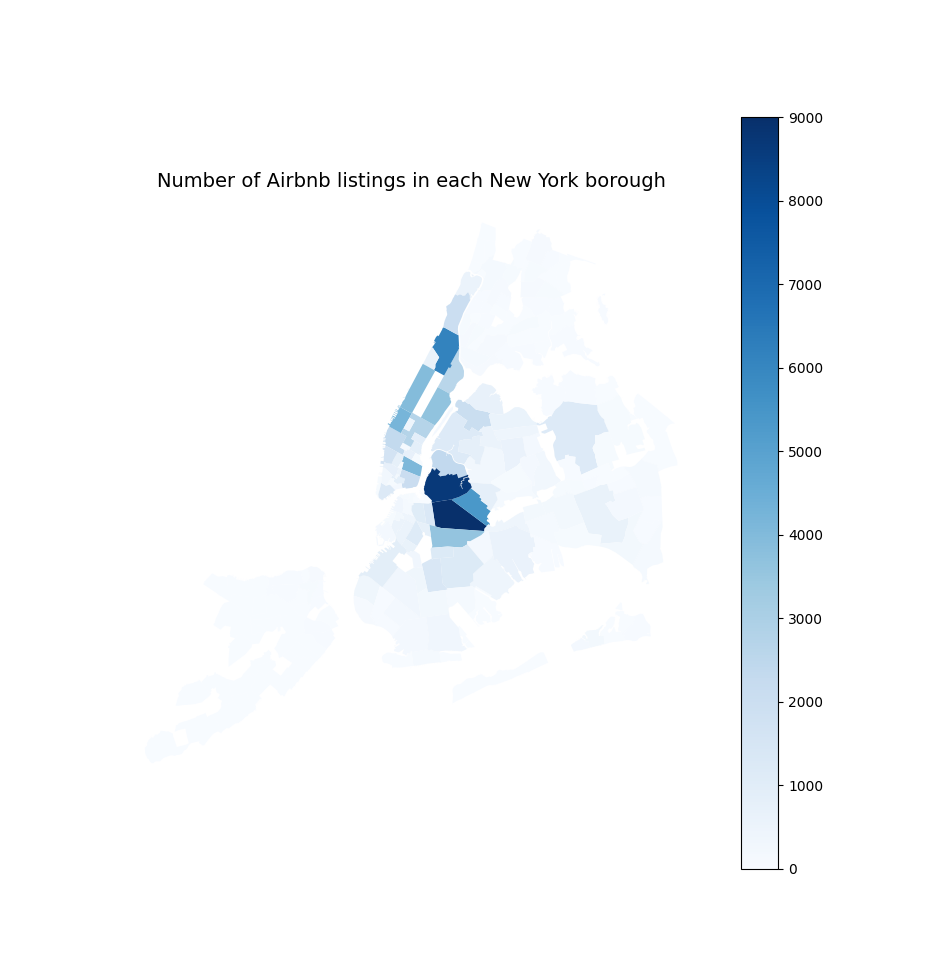
\includegraphics[width=\textwidth]{Figure_10.png}
%\end{figure}
\begin{figure}[H] \centering
\caption{Borough Listings}
    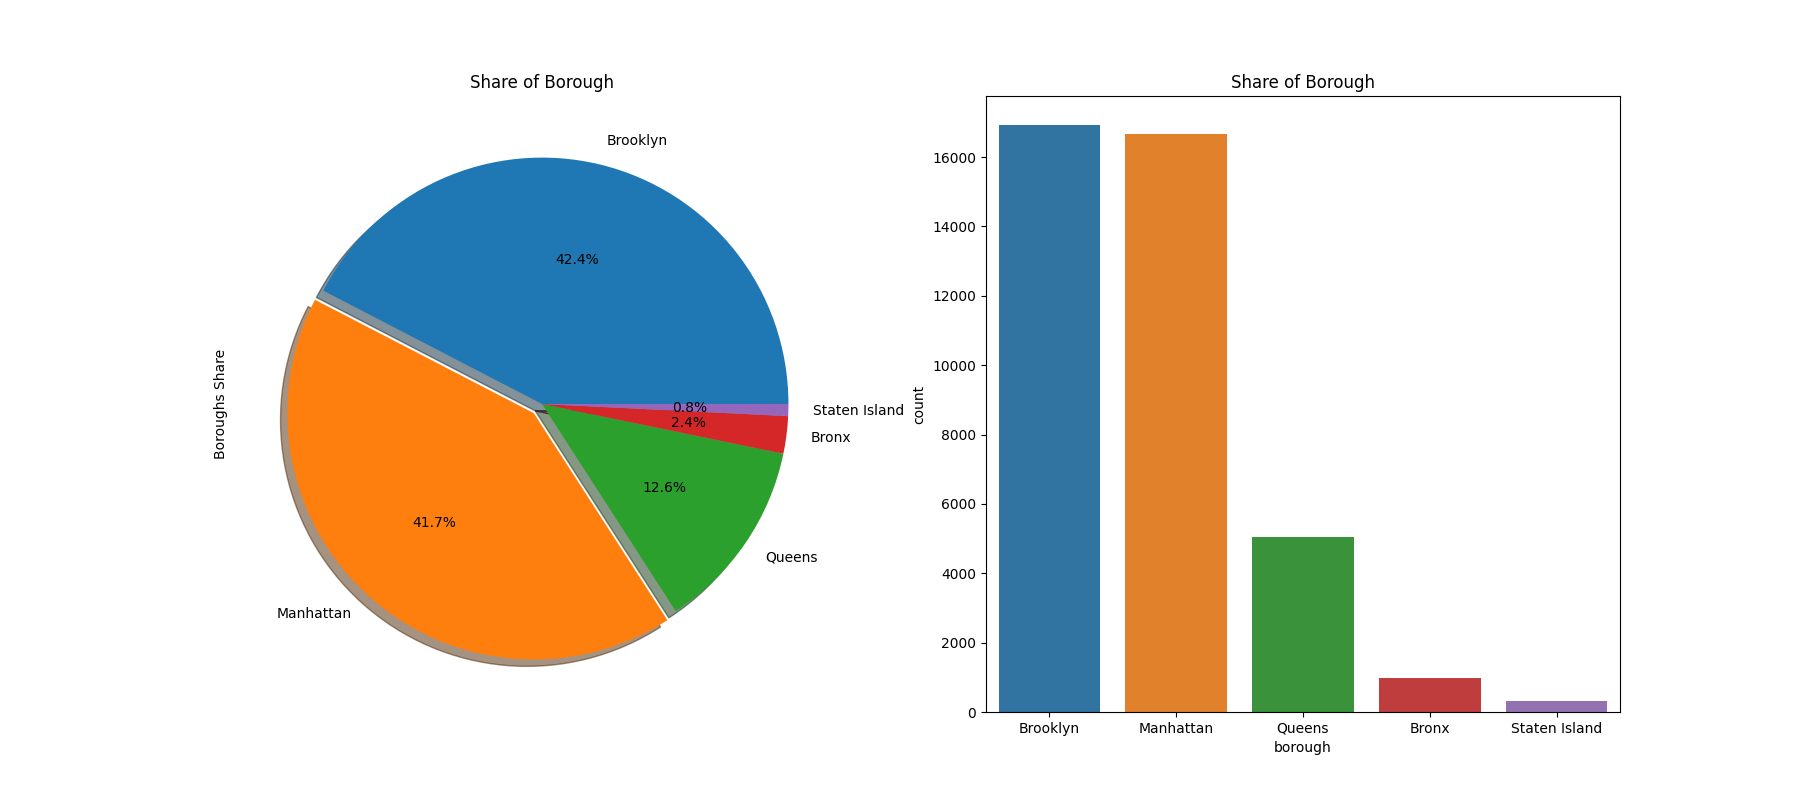
\includegraphics[width=0.75\textwidth]{Figure_10_b.png}
    \label{fig:borough-number-of-listing}
\end{figure}

Top ten neighbourhood with most listings:

\begin{figure}[H] \centering
\caption{Top 10 Neighbourhood with Most Listings}
    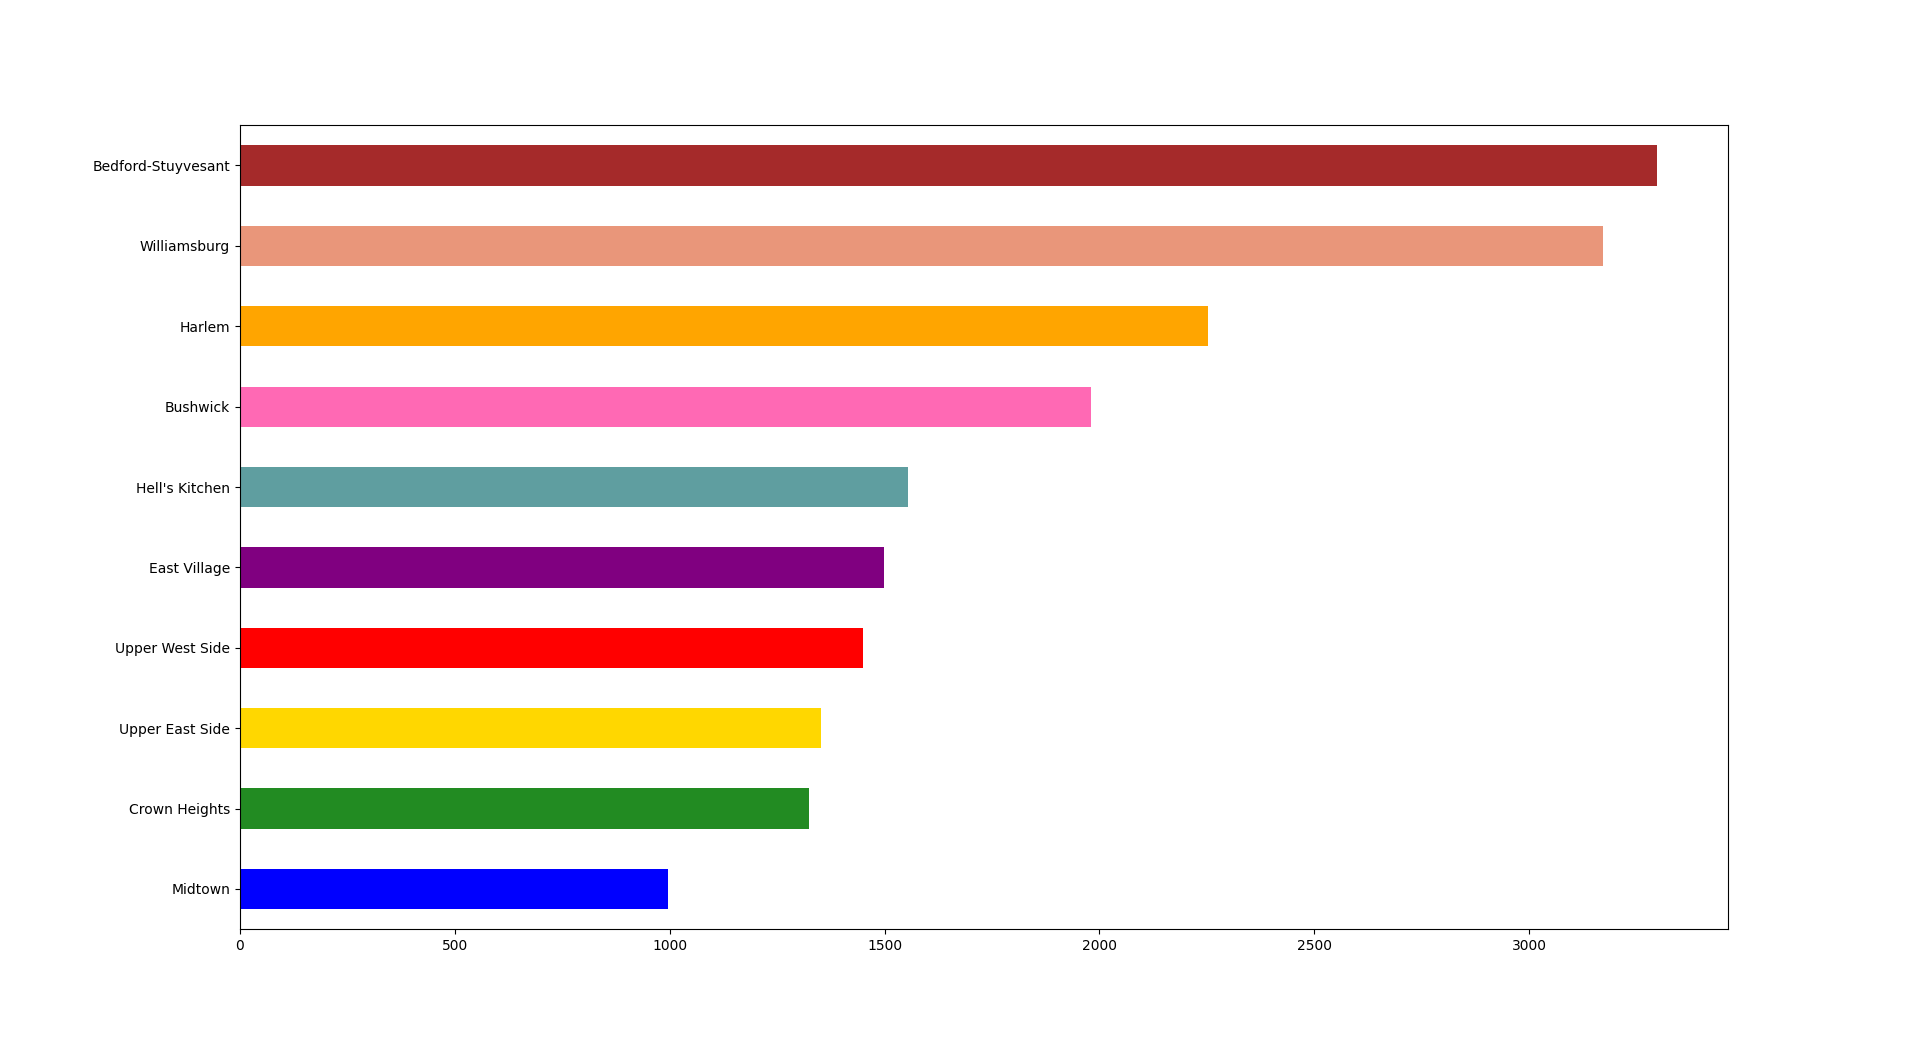
\includegraphics[width=\textwidth]{Figure_10_c.png}
    \label{fig:top-ten-most-listing-neighbourhood}
\end{figure}



As shown in Figure \ref{fig:median-price-borough} and Figure
\ref{fig:borough-price-distribution} , Unsurprisingly, Manhattan is the most
expensive borough - this is a famously expensive area to live, with some of the
world's highest house prices. The second most expensive area is in Brooklyn,
followed by Queens. Staten Island is the least expensive area to rent Airbnb
accommodation.

\begin{figure}[H]\centering
    \caption{Median Price of Airbnb listings in each New York borough}
    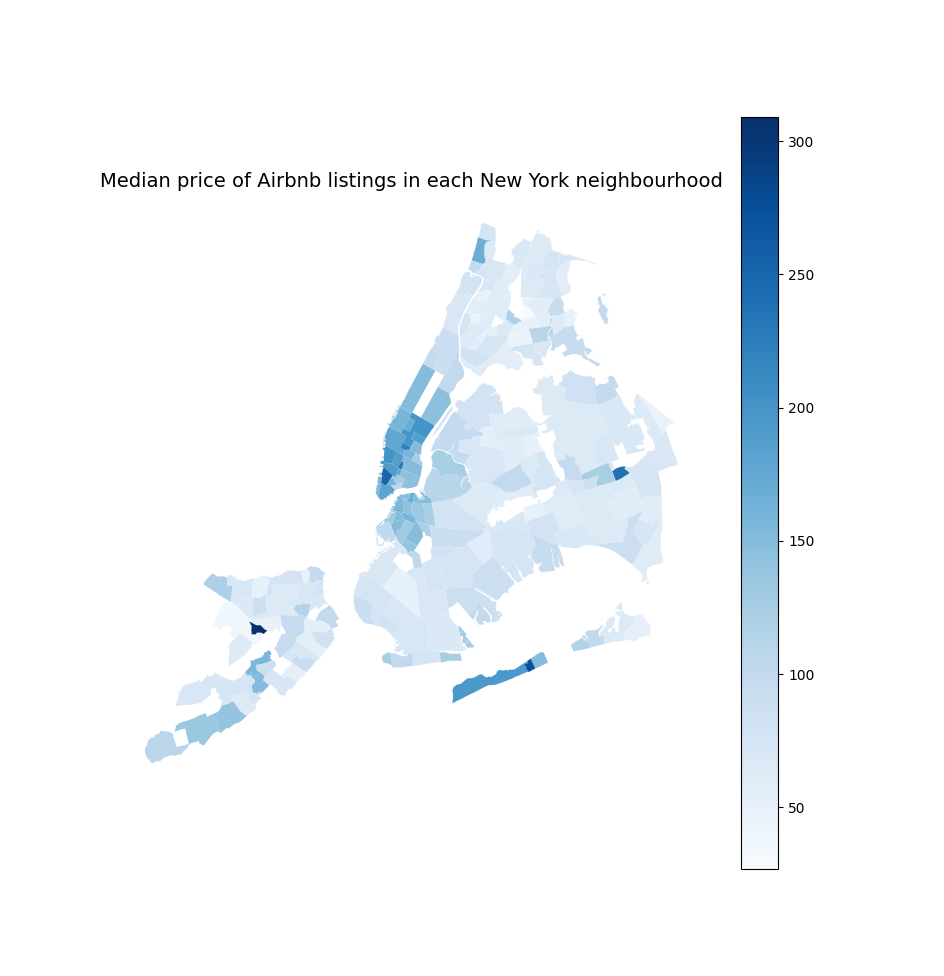
\includegraphics[width=0.75\textwidth]{Figure_11.png}
    \label{fig:median-price-borough}
\end{figure}

\begin{figure}[H]\centering
    \caption{Borough Price Distribution}
    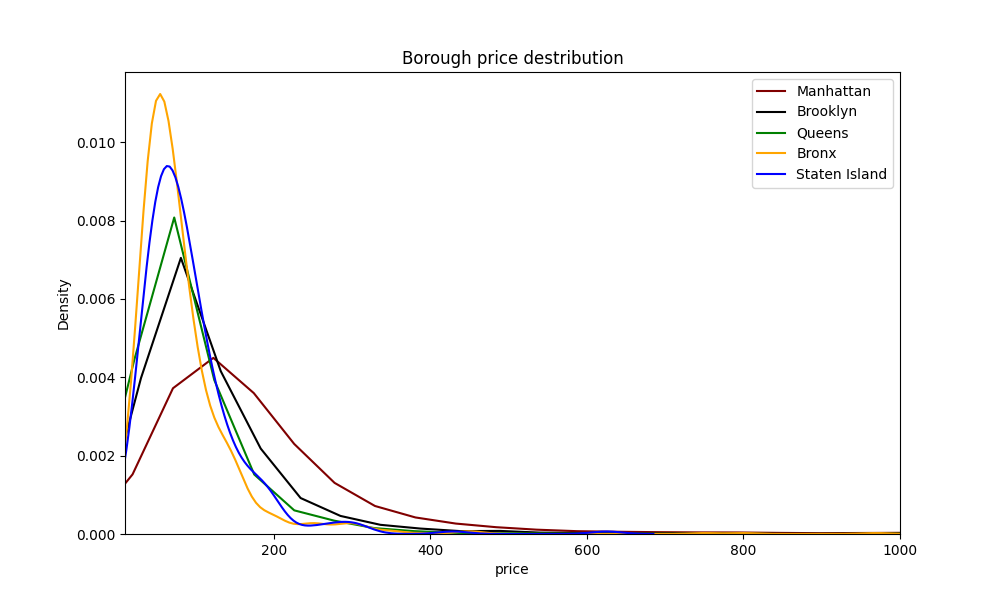
\includegraphics[width=0.75\textwidth]{Figure_11_b.png}
    \label{fig:borough-price-distribution}
\end{figure}

\subsection{Property and room types}

As shown in Figure \ref{fig:property_type},
about 80\% properties are apartments. The remainder are houses or more uncommon
property types (e.g. 'bed and breakfast' or 'yurt').

\begin{figure}[H]
    \centering
    \begin{subfigure}[b]{0.48\textwidth}
        \centering
        \caption{Property Type Pie Chart}
        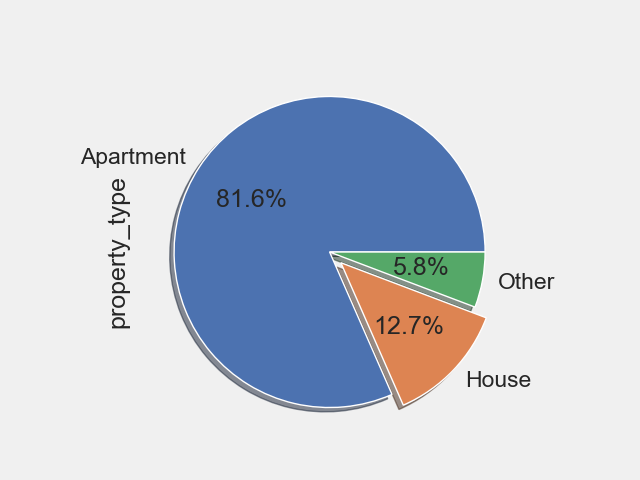
\includegraphics[width=\textwidth]{Figure_12_property_type_pie.png}
        \label{fig:property_type_pie}
    \end{subfigure}
    \begin{subfigure}[b]{0.48\textwidth}
        \centering
        \caption{Property Type Bar Chart}
        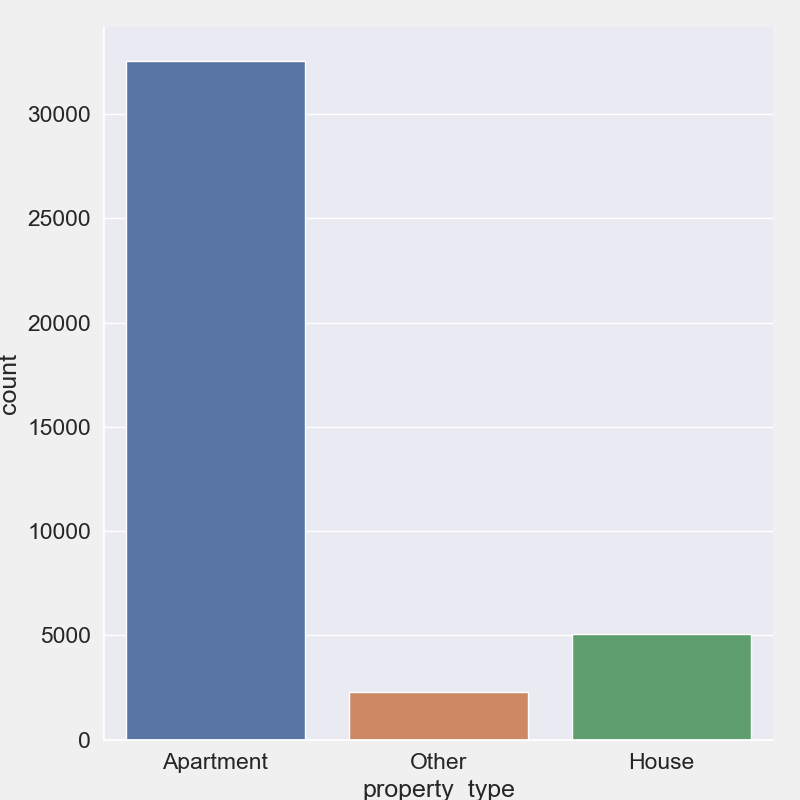
\includegraphics[width=\textwidth]{Figure_12_property_type.png}
        \label{fig:property_type_bar}
    \end{subfigure}

    \caption{Property Type}
    \label{fig:property_type}
\end{figure}

Figure \ref{fig:room_type} shows that about 52\% of listings are entire homes
(i.e. you are renting the entire property on your own). Most of the remainder
are private rooms (i.e. you are renting a bedroom and possibly also a bathroom,
but there will be other people in the property). Fewer than 3\% are shared rooms
(i.e. you are sharing a room with either the property owner or other guests).

\begin{figure}[H]
    \centering
    \begin{subfigure}[b]{0.48\textwidth}
        \centering
        \caption{Room Type Pie Chart}
        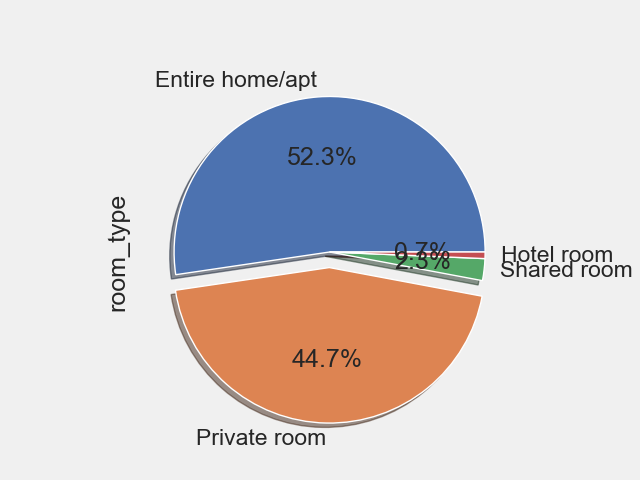
\includegraphics[width=\textwidth]{Figure_12_room_type_pie.png}
        \label{fig:room_type_pie}
    \end{subfigure}
    \begin{subfigure}[b]{0.48\textwidth}
        \centering
        \caption{Room Type Bar Chart}
        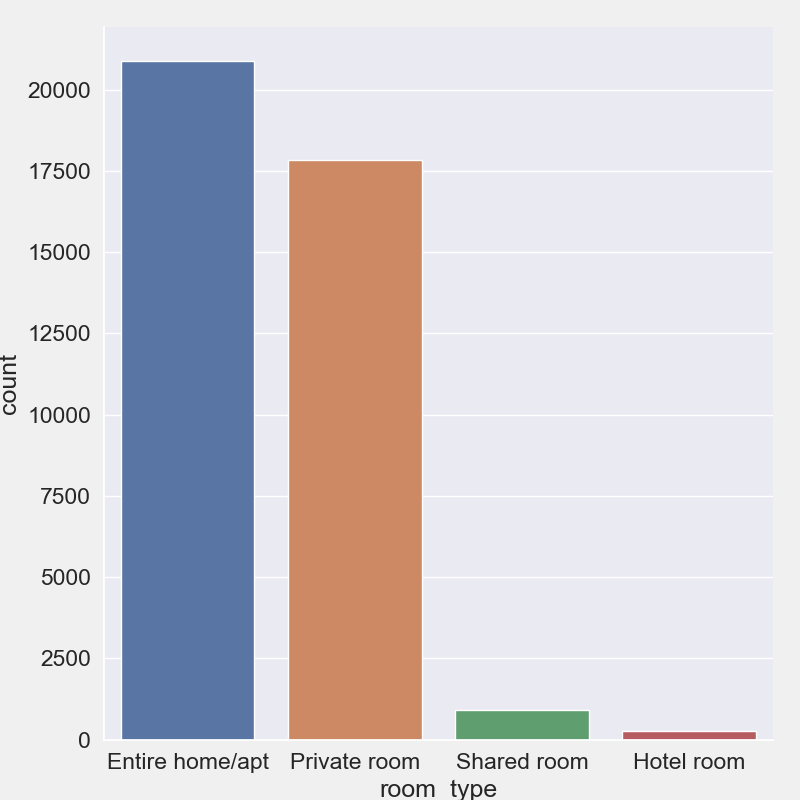
\includegraphics[width=\textwidth]{Figure_12_room_type.png}
        \label{fig:room_type_bar}
    \end{subfigure}
    \caption{Room Type}
    \label{fig:room_type}
\end{figure}

\subsection{Reviews}

From Figure   \ref{fig:overall-listing}, we see that, while few listings receive
review ratings of 80 or below, most listings with a review have received a
95-100/100 overall,  indicating that the customers adore their Airbnbs.

\begin{figure}[H]\centering
    \caption{Overall Listing Rating}
    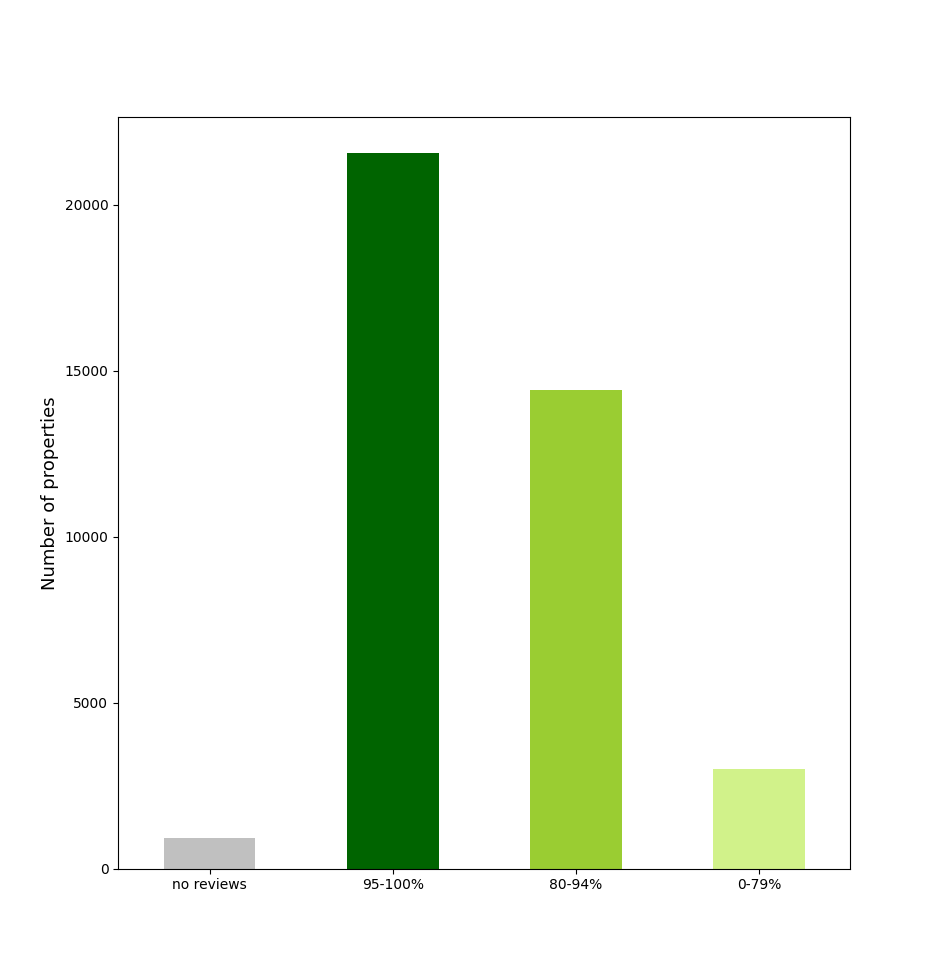
\includegraphics[width=0.75\textwidth]{Figure_13.png}
    \label{fig:overall-listing}
\end{figure}
%Figure \ref{fig:overall-listing-rating}

\subsection{First and Last Review}

As can be seen from the Figure ~\ref{fig:time_since_first_review}, the most
common period in which  Airbnb listings had their first review is 2-3 years,
which means that many listings on the site have been active for at least a
couple of years. However,  fewer listings have been on Airbnb for more than four
years.

The bar plot ~\ref{fig:time_since_last_review} reveals that the most
common period since a listing received its last review is 2-8 weeks, which means
that many listings have been reviewed relatively recently.  What stands out in
the figure is that over 10,000 listings have not had a review for more than a
year, which means they exist on the site, but they do not have their calendars
open and are not available to reserve.

\begin{figure}[H]
    \centering
    \begin{subfigure}[b]{0.48\textwidth}
        \centering
        \caption{Time Since First Review}
        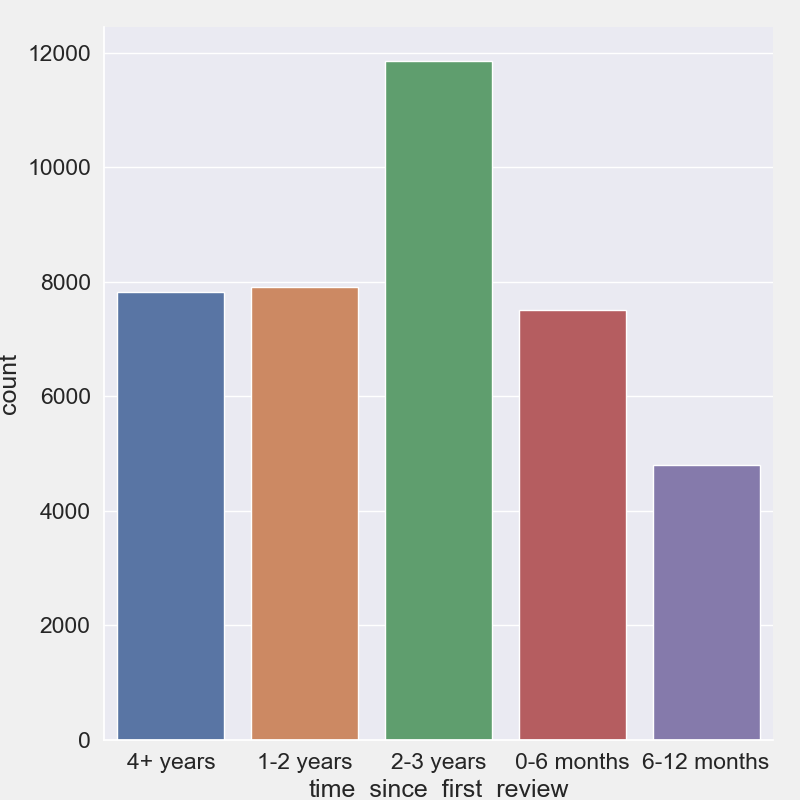
\includegraphics[width=\textwidth]{Figure_15_time_since_first_review.png}
        \label{fig:time_since_first_review}
    \end{subfigure}
    \begin{subfigure}[b]{0.48\textwidth}
        \centering
        \caption{Time Since Last Review}
        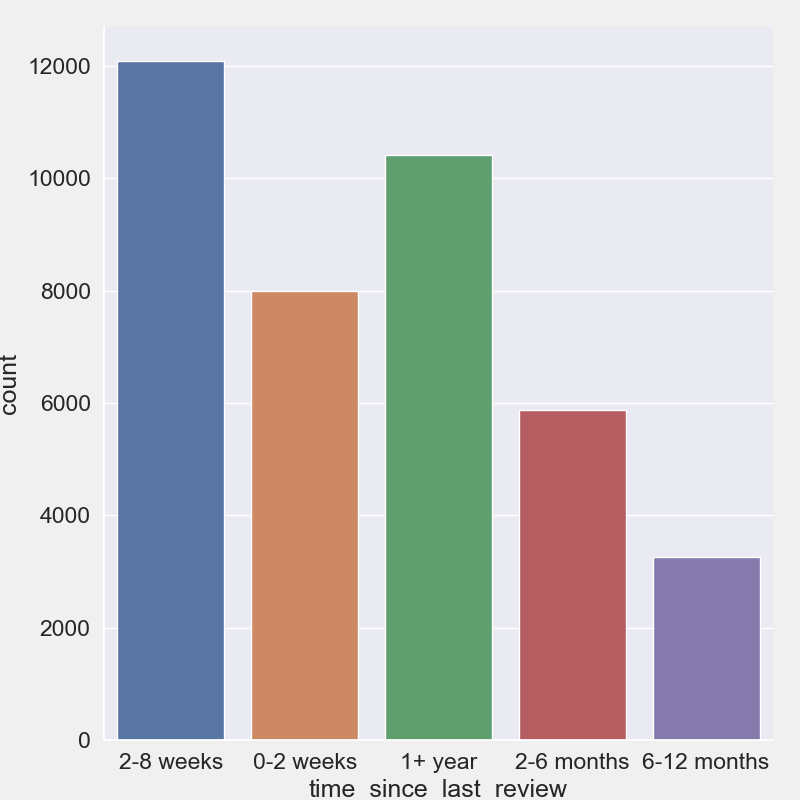
\includegraphics[width=\textwidth]{Figure_15_time_since_last_review.png}
        \label{fig:time_since_last_review}
    \end{subfigure}
    \caption{First and Last Review}
\end{figure}

\section{Boolean features}
\label{sec:boolean_features}

Many features (e.g. for amenities) can be true or false. This section compares
the proportions of these features that are true or false (to explore the data
and also to ascertain whether the feature is worth retaining), and the median
price of each category (to explore the relationship between the category and
price).

\subsection{Superhosts}

Figure ~\ref{fig:host_is_superhost} shows that about 23\% of hosts are "superhosts". As expect that being a superhost (a
mark of quality, requiring various conditions to be met)  improve the median
price of Airbnb listing.

\begin{figure}[H]\centering
    \caption{host\_is\_superhost}
    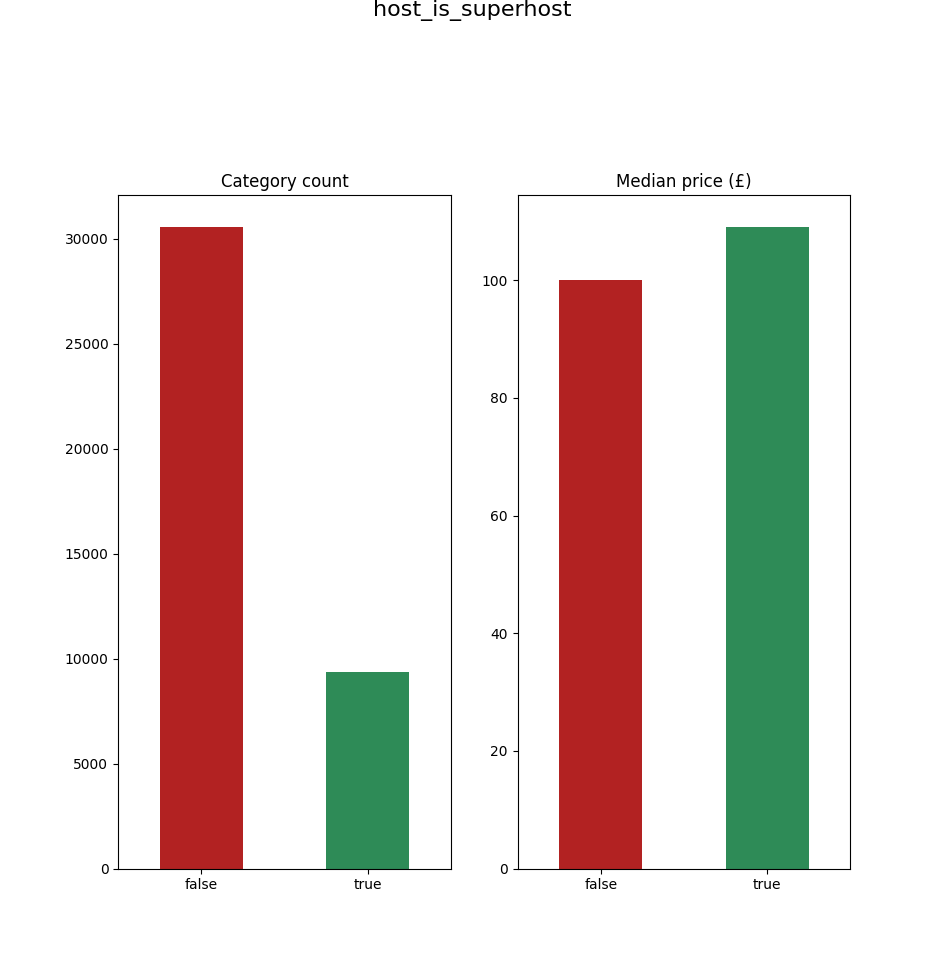
\includegraphics[width=0.75\textwidth]{Figure_16_host_is_superhost.png}
    \label{fig:host_is_superhost}
\end{figure}

\subsection{Host verification}

In Figure ~\ref{fig:host_identity_verified}, about 49\% of hosts are verified.
As with superhost, verifying host's profile (e.g. by providing ID and verifying
your phone number and email address) can lead to a price premium. The reason for
this may have something to do with the fact that providing host's verification
increases the trustworthiness of the host (Ert 2016).

\begin{figure}[H]
    \centering
    \caption{host\_identity\_verified}
    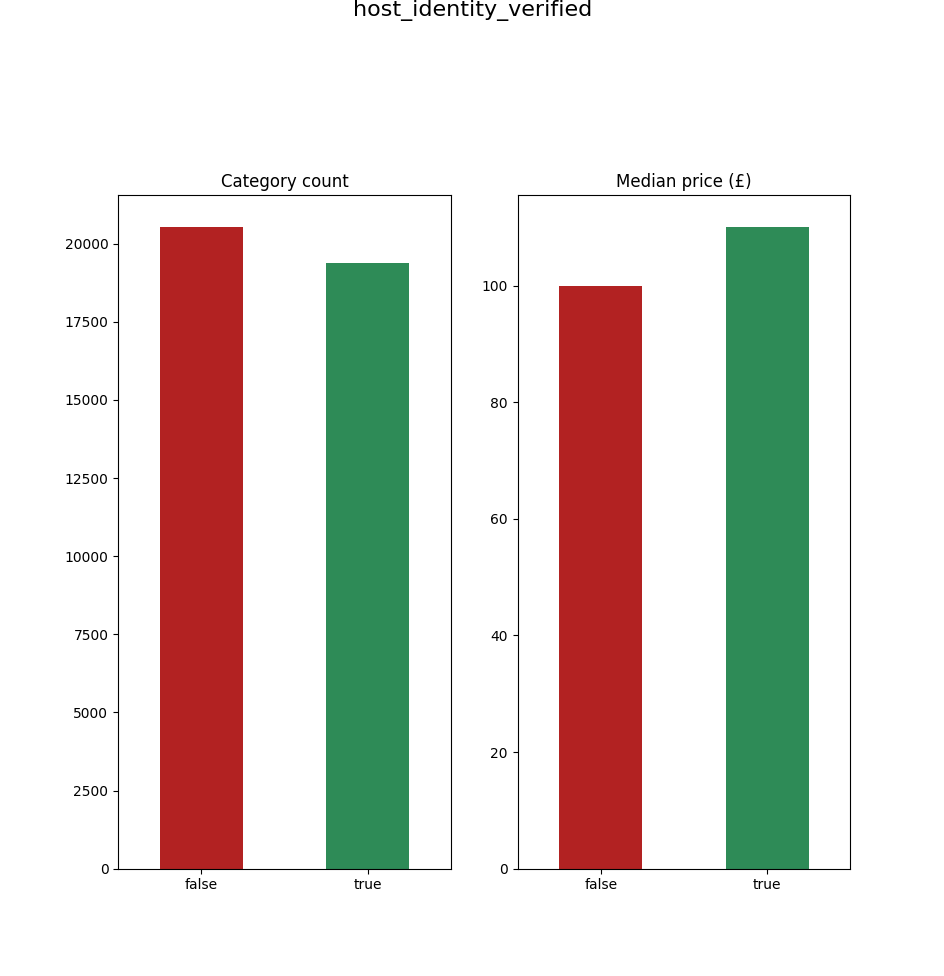
\includegraphics[width=0.75\textwidth]{Figure_16_host_identity_verified.png}
    \label{fig:host_identity_verified}
\end{figure}

\subsection{Instant booking}

As shown in figure below, about 40\% of properties are instant bookable. However, the added
convenience does not seem to have any effect on the median price per night. This
negative link can be explained by both emotional (Wang \& Nicolau 2017) and
economic (Benitez-Aurioles, 2018)

\begin{figure}[H]
    \centering
    \caption{instant\_bookable}
    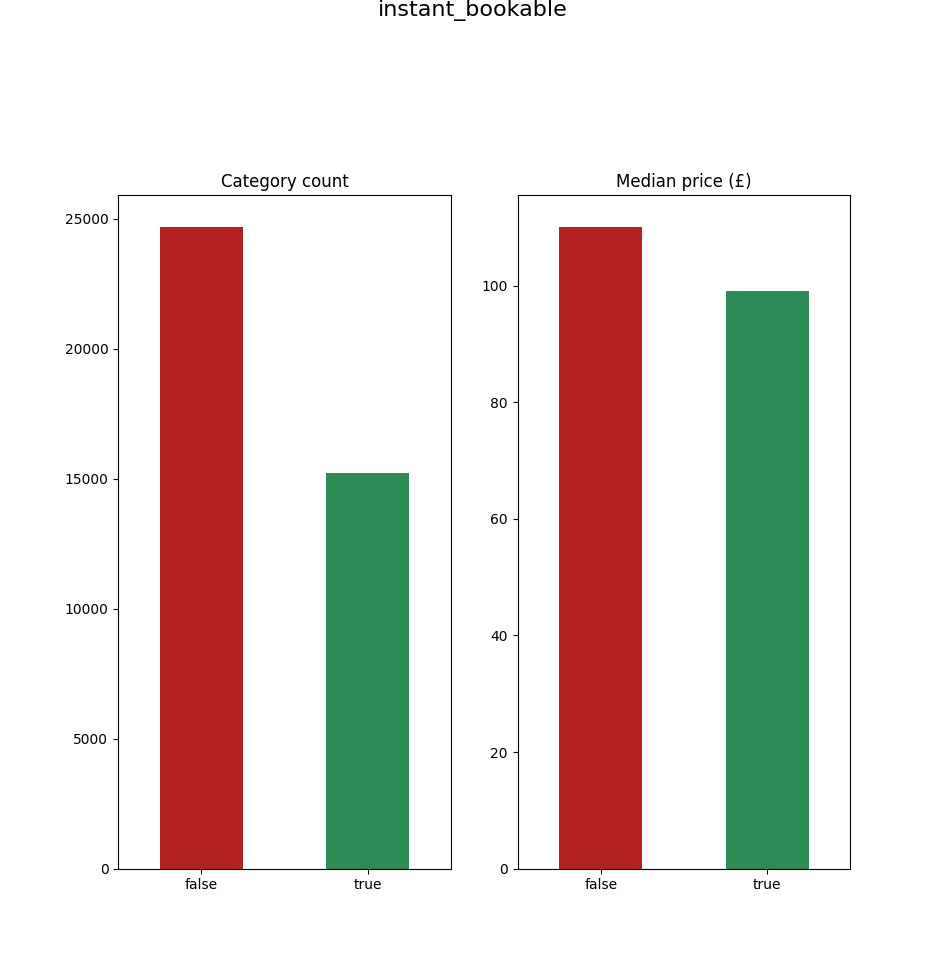
\includegraphics[width=0.75\textwidth]{Figure_16_instant_bookable.png}
    \label{fig:instant_bookable}
\end{figure}

\subsection{Amenities}

Our goal is to identify which amenities are common and which increase the price
of an Airbnb listing.  In Figure ABC, we plot the count plot and each amenity's
median price to explore the relationship between the amenity and price.
Amenities then can be split into three groups:

\begin{enumerate}

  \item The first group contains uncommon amenity, but listings with it have a
    higher median price: Bed linen, Coffee machine, Basic cooking equipment,
    Elevator, Child friendly, Long term stays allowed, Private entrance, Self
check-in, Pets allowed, Air conditioner

  \item The second group includes common amenities and listings with it have a
higher median price: TV, Washer, dryer and/or dishwasher (white goods), Internet

  \item The third group comprises uncommon amenities, and listings with it have
    a lower median price: Parking (presumably because these are less likely to
    be central properties), Greeted by host

\end{enumerate}

%\section{Time Series Analysis}
%\label{sec:time_series}

%Lorem ipsum dolor sit amet, consetetur sadipscing elitr, sed diam nonumy eirmod tempor invidunt ut labore et dolore magna aliquyam erat, sed diam voluptua. At vero eos et accusam et justo duo dolores et ea rebum. Stet clita kasd gubergren, no sea takimata sanctus est Lorem ipsum dolor sit amet.



\clearpage
\chapter{Data Modelling Methods}
\label{c:methods}
In this chapter, we discuss the concept of regression and related methods and
the role they play in predicting future housing prices. Regression analysis is a
statistical technique used to determine the contributing effect of a set of
explanatory variables on the response variable.

\section{Quantitative Measures of Performance}
Selecting the best method among many different statistical learning approaches
can be one of the practitioners' most daunting tasks.  One particular approach
may work best on a particular data set, but some other methods may perform
better on a similar but different data set.
Therefore, it is critical to select which method produces the best results for
any given data set.

To assess a particular model's predictive performance on a given data set, we
need some way to measure how well its predictions match the observed data.
\subsection{Mean Squared Error}
When
an outcome is a number (regression problem), the most commonly used method for
characterizing a model's predictive capabilities is to use the mean squared
error (MSE), which is:
\begin{eqnarray}
    \label{eqn:mse}
    MSE = \frac{1}{n} \sum_{i=1}^{n}(y_i - \hat{f}(x_i))^2
\end{eqnarray}
where $\hat{f}(x_i)$ is the prediction that $\hat{f}$ gives for the $i_{th}$
observation. If the predicted responses are very close to the actual responses,
the MSE will be small and vice versa.

\subsection{Coefficient of Determination}
We also use the coefficient of determination ($R^2$) to measure the proportion
of the information in the data explained by the model.  For example, an $R^2$
value of 0.8 means that the model can explain  80 percent of the outcome's
variation. An $R^2$ of 1 indicates that the regression predictions perfectly fit
the data. It should be noted that $R^2$ is a measure of correlation, not
accuracy.

\noindent $R^2$ is calculated as the correlation coefficient between the
observed and predicted values and squares it:
\[ R^2 = 1 - \frac{SS_{res}}{SS_{tot}}\]
where $SS_{res}$ is the sum of squares of residuals and $SS_{tot}$ is the total
sum of squares (proportion to the variance of the data)

\section{The Problem of Overfitting}
\label{sec:overfitting}
New technologies have changed how we collected data in various fields as diverse
as finance, commerce, and medicine in recent years.  It is not unusual to obtain
an almost unlimited number of feature measurements. We might expect it will always be better to use as many features as possible in
our model. In other words, we suppose that the best model is the most flexible
one. However, this is not always the case.  Fitting a  model with a large number
of features can lead to overfitting the data, which means that the model follows
the errors or noise too closely.  This type of model will usually have poor
accuracy when predicting a new sample.

To prevent overfitting, in this study we use less flexible fitting methods such
as penalized regression models as explained in
\ref{sec:penalized_regression_models}


\section{Linear Regression}
\label{sec:linear-regression}

Linear regression is a straightforward approach for supervised learning. In
particular, linear regression is a useful tool for predicting a quantitative
response. Linear regression has been around for a long time and is the topic of
numerous works of literature.  Linear regression can represent more than one
variable as input, but all the variables are linear correlated. This is in line
with the Hedonic Price Theory, which asserts that a product's price can be
regarded as a function of the measurable,utility-affecting attributes or
characteristics of the product \parencite{rosen1974hedonic}

According to hedonic pricing theory, an Airbnb accommodation listing is a bundle
of factors that impact the overall product's quality and provide consumers with
value and satisfaction.  Accordingly, a listing's price can be linked to the
presence or absence of specific items; it is a price proposal reflecting the
host's assumptions about implicit marginal prices of particular listing
characteristics.

The aim of ordinary least squares linear regression is to find the plane that
minimizes the sum-of-squared errors between the observed and predicted
response.
\begin{eqnarray}
SSE = \sum_{i=1}^{n}(y_i - \hat{y}_i)^2
\end{eqnarray}
where $y_{i}$ is the outcome and $\hat{y}_i$ is the model prediction of that
sample’s outcome.
It can be proven mathematically  that the optimal plane is
\begin{eqnarray}
    \label{eqn:optimal_plane}
    (X^TX)^{-1}X^{T}y
\end{eqnarray}
where \textbf{X} is the matrix of predictors, and y is the response vector.
Equation ~\ref{eqn:optimal_plane} is also known as $\hat{\beta}$ (“beta-hat”) in statistical texts
and is a vector that comprises the parameter estimates or coefficients for each
predictor. This quantity (~\ref{eqn:optimal_plane}) is easy to compute, and the coefficients are directly
interpretable

Given some minimal premises about the distribution of the residuals \footnote{
the error terms $\epsilon$ are independent, uncorrelated and normally
distributed with mean of zero and constant variance $\sigma^2$ (a.k.a.
homoskedasticity)}, it has conclusively been shown that the parameter estimates
that minimize SSE are the ones that have the least bias of all possible
parameter estimates (\textcite{graybill1976theory} ). Therefore, these estimates
minimize the bias element of the bias-variance trade-off.

In linear regression, overfitting is more likely to be a serious concern
\parencite{harrell2015regression}. When
there is little or no theory available to guide on selecting the predictors, we
want to include in our model as many features as possible. However, we run the
risk of including irrelevant features that actually have no relation to the
dependent variable being predicted, thus might not improve the prediction
performance.

\section{Penalized Regression Models}
\label{sec:penalized_regression_models}

Penalized regression models shrink the size of multiple linear regression
coefficients, thus introducing bias, while attempting to improve the prediction.

\subsection{Ridge Regression}

%Originally proposed in 1970 by Arthur E. Hoerl and Robert W. Kennard, ridge
%regression attempts to correct for overfitting through regularization.
When the model overfits the data or issues with collinearity,
the linear regression parameter estimates may become inflated.  We want to find
a method to control the magnitude of these estimates to reduce the SSE.
One possible solution is to use Ridge Regression (\textcite{hoerl1970ridge})  to
control (or regularize) the parameter estimates by adding a penalty to the SSE
if the estimates become large.
%by adding a penalty on the sum of the squared
%regression parameters, often called L2 parameter.

Ridge regression is very similar to least squares, except that the coefficients
ridge are estimated by minimizing a slightly different quantity. In particular,
the ridge regression coefficient estimates $\hat{\beta}^R$ are the
values that minimize:
\begin{eqnarray}
    \label{eqn:ridge-optimal}
    \sum_{i=1}^{n}(y_i -\beta_0 - \sum_{j=1}^{p}\beta_j x_{ij}) ^ 2 + \lambda
    \sum_{j=1}^{p}\beta_{j}^2 = RSS + \lambda \sum_{j=1}^{p}\beta_{j}^2
\end{eqnarray}
In  Equation  ~\ref{eqn:ridge-optimal} we made a trade-off between two different
criteria. As with least squares, ridge regression seeks coefficient estimates
that fit the data well, by making the RSS small. But, the second term, $\lambda
\sum_{j=1}^{p}\beta_{j}^2$ signifies that a second-order penalty (i.e., the
square) is being used on the parameter estimates.
This shrinkage penalty is small when $\beta_1$,...,$\beta_p$ are close to zero,
and so it has the effect of shrinking penalty the estimates of $\beta_j$ towards
zero.

When $\lambda = 0$, the penalty term has no effect, and ridge regression is the same
as least squares estimates. However, as $\lambda \to \infty$, the influence of
the shrinkage penalty increases, and the ridge regression will shrink the
estimates towards  zero.
In contrast to least squares, which produces only one set of coefficient
estimates, ridge regression will generate a different set of coefficient
estimates, $\hat{\beta}_{\lambda} ^ {R}$, for each value of $\lambda$.

\subsection{Lasso Regression}
One drawback of ridge regression that it does not shrink any of the parameter
estimates towards 0. Therefore, the model does not conduct feature selection.

\noindent Least Absolute Shrinkage and Selection Operator (Lasso)
\parencite{tibshirani1996regression} model is a modern
alternative to ridge regression that overcomes this disadvantage. The name comes
from its functionality that it does not only shrink coefficients towards zero,
but it also performs feature selection.


The lasso  coefficients, $\hat{\beta}^L$ , minimize the quantity:
\begin{eqnarray}
    \label{eqn:lasso-optimal}
    \sum_{i=1}^{n}(y_i -\beta_0 - \sum_{j=1}^{p}\beta_j x_{ij}) ^ 2 + \lambda
    \sum_{j=1}^{p} \mid \beta_{j} \mid= RSS + \lambda \sum_{j=1}^{p} \mid \beta_{j} \mid
\end{eqnarray}
Notice that the lasso and ridge regression have similar formulations. The only distinction is in the penalty term. In particular, the $\beta_j^2$ term in the ridge regression penalty (6.5) has been replaced by $\mid \beta_{j} \mid$ in the lasso penalty
The implication of this modification is that penalizing the absolute values has the effect of setting some of the coefficient estimates to be exactly equal to zero for some value of $\lambda$. Thus the lasso yields models that simultaneously use regularization to improve the model and to conduct feature selection.

We can formulate the lasso and ridge regression coefficient estimates in
\ref{eqn:lasso-optimal} and \ref{eqn:ridge-optimal} as solving following
problems:

\begin{equation}
    \label{eqn:ridge-optimal}
    \begin{aligned}
    \min_{\beta} \quad \sum_{i=1}^{n}(y_i -\beta_0 - \sum_{j=1}^{p}\beta_j
    x_{ij}) ^ 2  \quad \textrm{subject to} \quad \sum_{j=1}^{p}\mid\beta_j\mid
    \leq s
    \end{aligned}
\end{equation}
and
\begin{equation}
    \label{eqn:lass-optimal}
    \begin{aligned}
    \min_{\beta} \quad \sum_{i=1}^{n}(y_i -\beta_0 - \sum_{j=1}^{p}\beta_j
    x_{ij}) ^ 2  \quad \textrm{subject to} \quad \sum_{j=1}^{p}\beta_j^2\leq s
    \end{aligned}
\end{equation}

In the figure \ref{fig:feature-selection}, we illustrate why the lasso performs
feature selection, while ridge regression does not.To simplify the problem, we
consider only two parameters $\beta_1$ and $\beta_2$.
The elliptic centered around $\hat{\beta}$ are contours of the sum of squares
error with the OLS estimator in the center. All of the points on a given ellipse
has the same value of RSS. The diamond and circle represent the lasso and ridge
regression constraints in \ref{eqn:lasso-optimal} and \ref{eqn:ridge-optimal}.

The lasso and ridge regression coefficient estimates are the first point at
which an ellipse touches the constraint set.
Note that the ridge regression has a circular constraint with no sharp points.
This intersection will not generally occur on an axis. So the ridge regression
coefficient estimates will be exclusively non-zero. However, the lasso
constraint has corners at each of the axes, and so the ellipse will often
intersect the constraint region at an axis. When this occurs, one of the
coefficients will equal zero.In this way, the lasso performs \textit{feature
selection}.
\begin{figure}[H]\centering
    \caption{Illustration of two dimensional case of estimation for the lasso
    (right) and the ridge regression}
    \label{fig:feature-selection}
    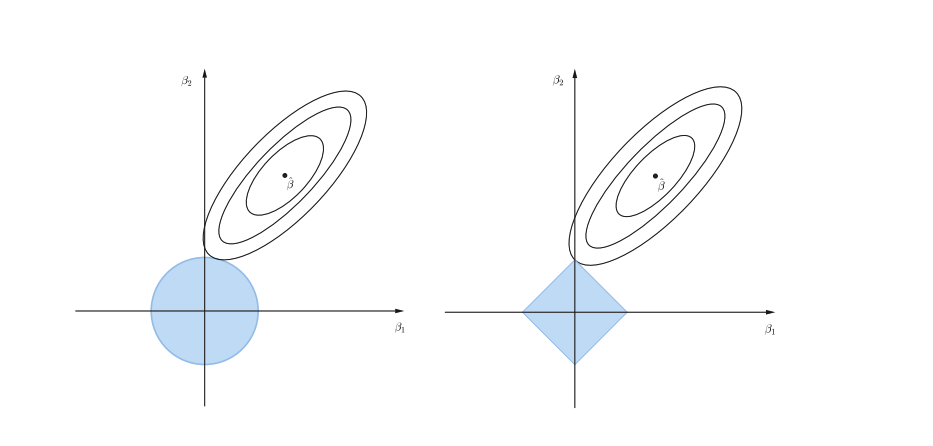
\includegraphics[width=\textwidth]{feature-selection.png}
\end{figure}
\vspace{1mm}
\subsection{Selecting the Tuning Parameter}

Choosing an optimized value of tuning parameter $\lambda$ is critical when
implementing the ridge and the lasso regression.
We do not want to choose $\lambda$ too small due to the low restriction. On the
other hand, when $\lambda$ is very large, the restriction is more substantial
than it is desired. We handle the problem of the optimal value of  by using a
cross-validation technique. \textcite{efron1994introduction} introduce the algorithm, which describes
the procedure of cross-validation.

\begin{algorithm}[H]
\setstretch{1.35}
\SetAlgoLined
\renewcommand{\labelenumi}{(\Roman{enumi})}
Split the data into K roughly equal-sized parts.

For the $k^{th}$ part, fit the model to the other K − 1 parts of the data, and
calculate the mean squared error of the fitted model when predicting the
$k^{th}$ part of the data.

Repeat step 2 for k = 1, 2, . . . , K and average the K estimates of mean
squared error $MSE_1$, $MSE_2$,..., $MSE_k$.

For each tuning parameter value $\lambda$, compute the average error over all
folds \[CV_{(k)} = \frac{1}{k} \sum_{i=1}^{k} MSE_i\]

 \caption{K-Fold Cross Validation}
\end{algorithm}


We choose a grid of $\lambda$ values and calculate the cross-validation error
for each value of $\lambda$. We then select the tuning parameter value for which
the cross-validation error is smallest.


\section{XGboost}

All the approaches reviewed so far suffer from the fact that they use a single
model for predicting the response variable. Hence the ability to choose a
suitable model is crucial to have any chance to obtain good results.

\noindent Machine Learning practitioners have to consider many factors such as
the quantity of data, the dimensionality of the space, and distribution
hypothesis to find a high predictive power model.

Using this approach, we have to face the bias-variance tradeoff. On the one
hand, we want our model to have enough degrees of freedom to resolve the
underlying complexity of the data we are working with. On the other hand, we
also want it to have not too many degrees of freedom to avoid high variance and
be more robust.

Boosting, on the other hand, takes a more iterative approach. It is an ensemble
technique in which several models are combined to achieve a better one.

\subsection{Ensemble Methods}

Imagine we want to buy a new laptop. We are unlikely to walk into a store and
buy a laptop. You search the product on the internet, read reviews, compare
models, prices. We ask for opinions from our family and friends. In brief, we
investigate, seek the \textit{wisdom of the crowd} before making an informed
decision.\newline
Likewise, if we combine multiple learning algorithms, we will often obtain
better predictions than the best individual algorithm. We call a group of
predictors an \textit{ensemble}, and the technique is called Ensemble Learning. The
Ensemble Learning algorithm is called an Ensemble method.

In practice, two ensemble models have proven to be effective on a wide range of
datasets for classification and regression, both of which use decision trees as
their building blocks: random forests and gradient boosted decision trees.

%\subsection{Boosting}
\subsection{Gradient Boosting}

While there are several boosting methods available, the two most popular are
Adaptive Boosting \autocite{freund1997decision} and Gradient
Boosting \autocite{friedman2001greedy}. In this study, we focus on Gradient
boosting trees and its high-performance implementation, XGBoost.
The Gradient boosting trees model uses a regression tree as the base learner.
\citeauthor{kuhn2013applied} \parencite{kuhn2013applied} suggests three reasons
why trees make an excellent base learner for boosting:
\begin{enumerate}
    \item By limiting their depth, they can be weak learners.
    \item We can add together separate trees easily.
    \item Trees can be created quickly.
\end{enumerate}

The basic gradient boosting regression principles are: given mean squared error
( a loss function ) and regression trees (weak learners). The goal of Gradient
Boosting Trees is to find an additive model that minimizes the loss function.

We illustrate this approach in Figure ~\ref{fig:gradient-boosting-illustration}

\begin{figure}[H]\centering
    \caption{Gradient Boosting Approach}
    \label{fig:gradient-boosting-illustration}
    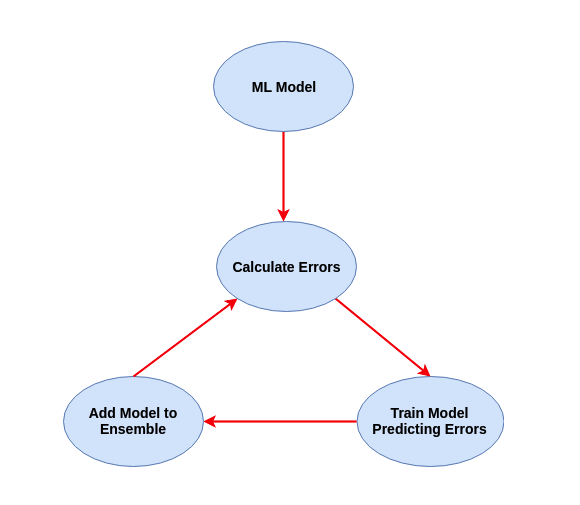
\includegraphics[width=\textwidth]{gradient-boosting-illustration.png}
\end{figure}

\textcite{kuhn2013applied} illustrate the Gradient Boosting for
Regression algorithm as followed:

\begin{algorithm}[H]
\setstretch{1.35}
\SetAlgoLined

\renewcommand{\labelenumi}{(\Roman{enumi})}
Select tree depth, D, and number of iterations, K

Compute the average response, $\bar{y}$, and use this as initial predicted value for each sample

\For{$k\gets0$ \KwTo $K$ }{
    Compute the residual, the difference between observed value and the \textit{current} predicted value, for each sample

    Fit a regression tree of depth, D, using the residuals as the response

    Predict each sample using regression fit in the previous step

    Update the predicted value of each sample by adding the previous iteration's predicted value to the predicted value generated in the previous step

    }
 \caption{Simple Gradient Boosting for Regression}
\end{algorithm}
\subsection{XGBoost}
Extreme Gradient Boosting (XGBoost) is a variant of the gradient tree boosting.
Gradient boosting and XGBoost follows the same principle. The key differences
between them lie in implementation details.
Specifically, features of XGBoost which make it stand out of from the rest of
other gradient boosting algorithms, are
\begin{itemize}
    \item Clever penalization of trees
    \item A proportional shrinking of leaf nodes
    \item Newton Boosting
    \item Extra randomization parameter
    \item Implementation on single, distributed systems and out-of-core computation
\end{itemize}
%Several reasons explain why XGBoost is popular in the machine learning
%community, which includes:
Besides these superior features, there are other reasons why XGBoost is getting
popular in the machine learning community:
\begin{itemize}
    \item Can solve a wide range of applications such as regression,
        classification, ranking, and user-defined prediction problems.
    \item Portability: Runs smoothly on Windows, Linux, and OS X.
    \item Languages: Supports all major programming languages, including C++,
        Python, R, Java, Scala, and Julia.
    \item Cloud Integration: Supports AWS, Azure, and Yarn clusters and works
        well with Flink, Spark, and other ecosystems.
\end{itemize}

Since its introduction in 2014, this algorithm has
been credited with winning numerous Kaggle competitions and being the driving
force under the hood for several cutting-edge industry applications. Futhermore,
XGBoost has been shown to provide state-of-the-art results for diverse problems,
including web text classification, customer behavior prediction, motion
detection, and malware classification \textcite{chen2016xgboost}
\textcite{nielsen2016tree}.

While XGBoost is suitable for predicting, it does so at the expense of its
interpretability.  As shown in Figure
\ref{fig:flexibility-interpretability-tradeoff}, compared to restrictive models
such as Lasso or Least Squares, Boosting is a highly flexible (complex) approach
that is harder to interpret.

\begin{figure}[H]\centering
    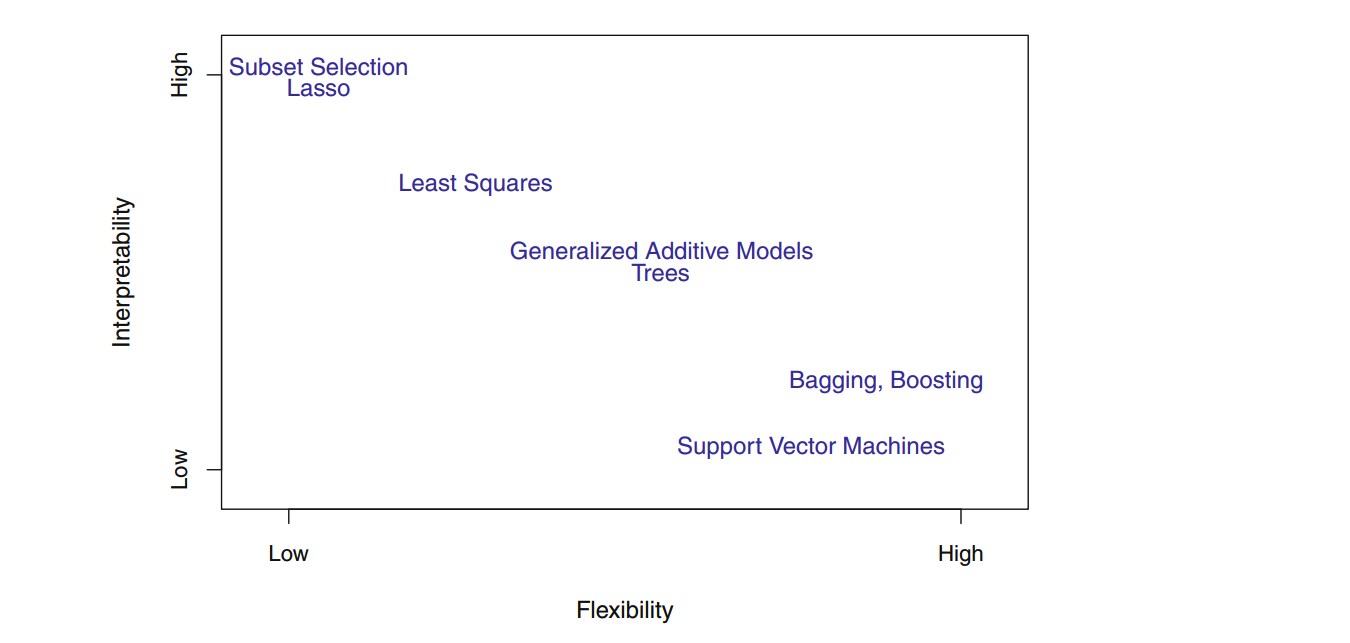
\includegraphics[width=0.75\textwidth]{flexibility-interpretability-tradeoff.png}
    \caption{Interpretability and Flexibility Tradeoff}
    \label{fig:flexibility-interpretability-tradeoff}
    \source{\textcite{james2013introduction}}
\end{figure}



\clearpage
\chapter{Experiments and Results}
\label{c:results}
In this chapter, we discuss the application of the methods from Chapter ~\ref{c:methods}
to the New York AirBnB dataset from Chapter  ~\ref{c:dataset}

\section{Training and Test Sets}
\label{sec:train_test_split}
We split the dataset into 80 listings (80\%) and 20 (20\%) listings for training
and test sets, respectively.  First, we built a model on the training data, and
then we test its performance on the test set.

Typically, we are not interested in how well the method works on the training
data. Instead, our goal is to assess the predictive accuracy we get when
applying our method to previously unseen test data. In other words, we want to
test the model's generalizability.  Normally, the test set is a smaller dataset
than the training set, which the model did not see previously.  Moreover, The
data splitting has to be unbiased. In particular, we have to randomly sample the
data to guarantee that the testing and training sets are similar in terms of
variation and representative.

We implement the data splitting by using the train\_test\_split() function from
sklearn

\section{Results}
\label{sec:results}

\subsection{Best Performance Model}
\label{ssec:cross-validation}

A summary of of results is reported in Table ~\ref{tab:results}

\begin{table}[htpb]
  \centering
  \caption{Results}
  \label{tab:results}
  \begin{tabular}{lllll}
    \hline
    ML Algorithm & Training MSE & Test MSE & Training $R^2$ & Test $R^2$ \\
    \hline
    Linear Regresion & 0.1291 &  8.5E21 &  0.7019 & -1.9E22 \\
    Ridge Regression  & 0.1291 & 0.138 & 0.7019 &  0.6857 \\
    Lasso Regression & 0.1351 & 0.1441 & 0.688 & 0.6718 \\
    XGboost &  0.0798 & 0.1173 & 0.8157 &  0.7328 \\
  \end{tabular}
\end{table}

\subsection{Linear Regression}

As expected in \ref{sec:linear-regression}, incorporating such a large number of
features (309) makes the linear regression model overfit the data. As shown in
Table ~\ref{tab:results}, while training MSE of the linear regression model is
quite good, the model performs poorly on the test set both in terms of   in
terms of $MSE$ and $R^2$

\subsection{Ridge Regression}

By performing k-fold cross-validation with ten folds, we can find the tuning
parameter's value that results in the smallest cross-validation error is 115.
The test's MSE is associated with this value of  is 0.138.  The result
represents a considerable improvement of ridge regression over the test MSE we
got using least square regression.


\subsection{Lasso Regression}

Using cross-validation as described in \ref{ssec:cross-validation}, we find the
optimized penalty value $\lambda$ is 0.005. The associated test MSE is 0.1441,
which is slightly higher than the test set MSE of the ridge regression.  Recall
from that the advantage of using lasso regression over ridge regression is that
lasso performs feature selection.
Lasso picked 153 variables while eliminated the other 125 features.
The figure ~\ref{fig:lasso-feature-importantance} shows the top 20 important features.

\begin{figure}[H]\centering
    \caption{Lasso Feature Importance}
    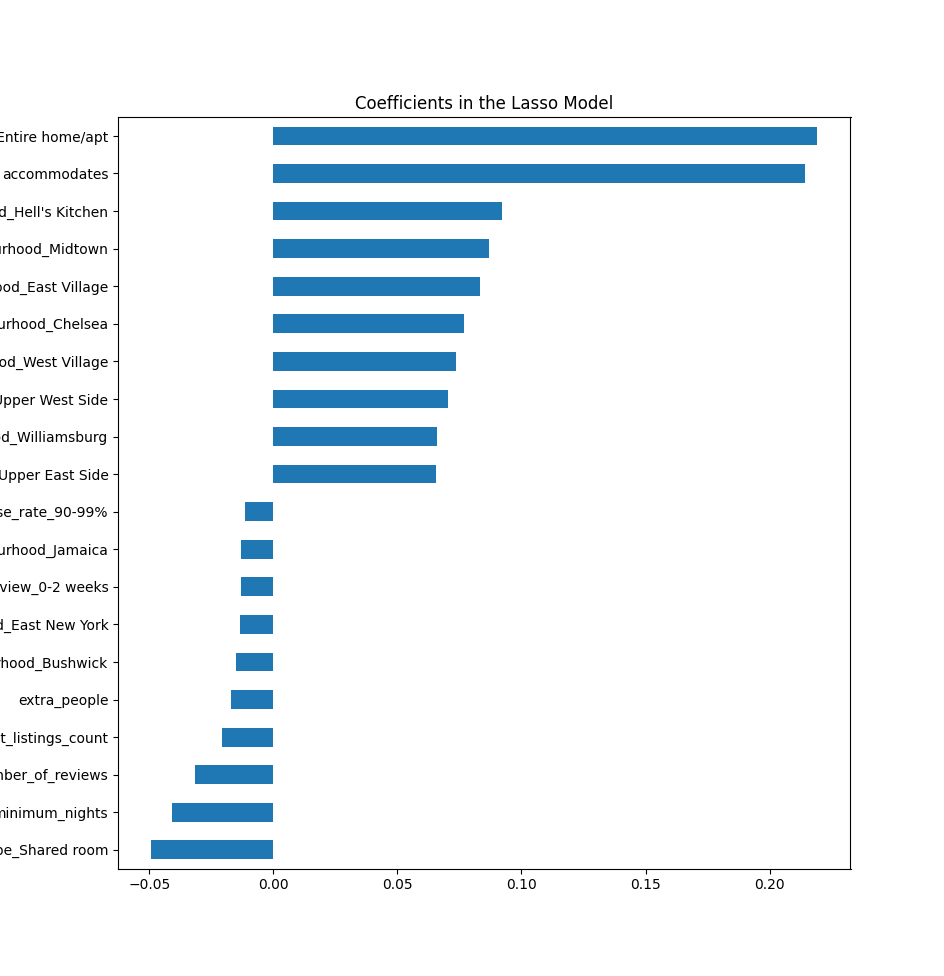
\includegraphics[width=\textwidth]{Figure_19.png}
    \label{fig:lasso-feature-importantance}
\end{figure}


It is not surprising that the two most important positive features are whether
the type of listing is the entire home and how many people the property
accommodates. These are the main things a customer would use to search for
properties in the first place.
Features related to the location are in the top 10.  Being in  Hell's
Kitchen, Midtown, East Village, Chelsea, West Village, Upper West Side,
Williamsburg, Upper East Side, SoHo, Lower East Side neighbourhood is associated
with an increase in the listing price.

\subsection{XGboost}

As shown by the Table ~\ref{tab:results}, XGboost consistently outperforms these
competing approaches in both mean squared error and R-squared.  With this model,
the features explain approximately 73\% of the target variable's variance and
have smaller MSE than the other regression model.

%Apart from its superior performance, another advantage of applying ensembles of
%decision tree methods like gradient boosting is that they can automatically
%provide estimates of feature importance from a trained predictive model.
%as shown in Figure ~\ref{fig:xgboost-feature-importantance}.
%\begin{figure}[h]\centering
    %\caption{XGboost Feature Importance}
    %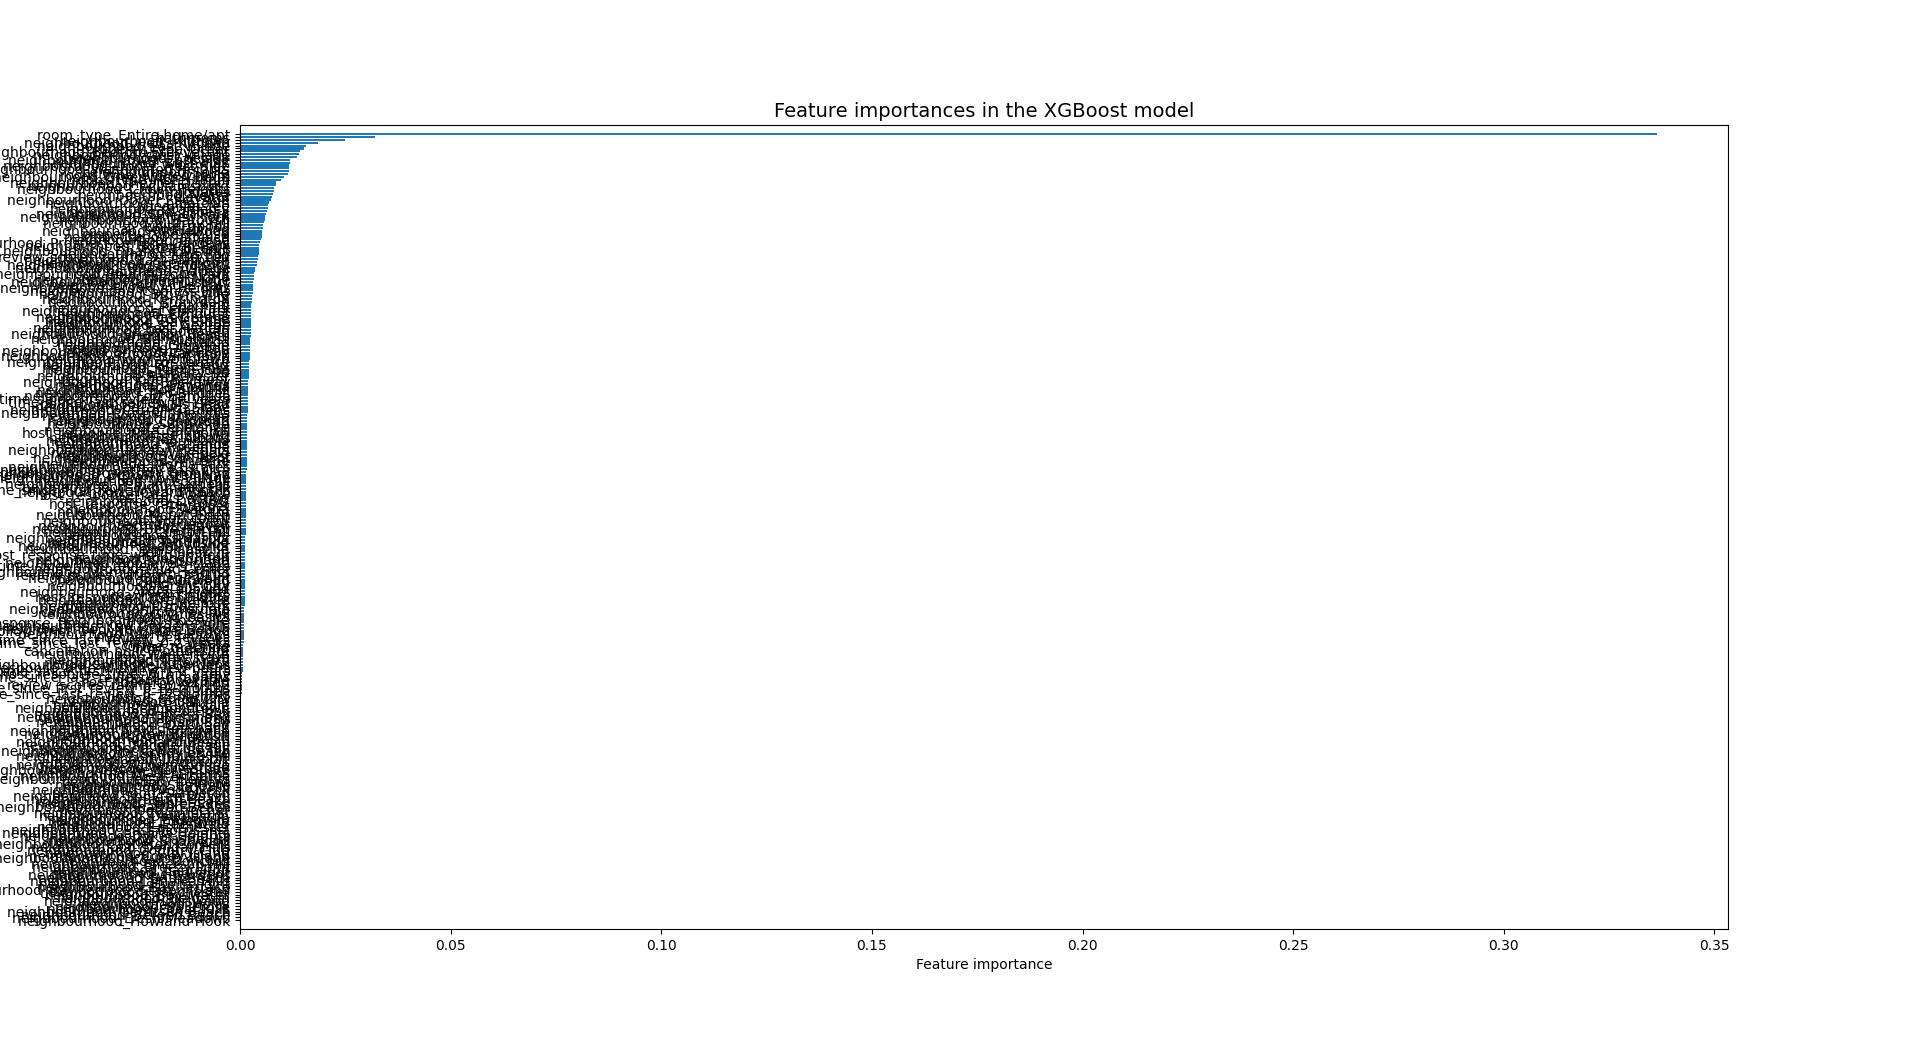
\includegraphics[width=\textwidth]{Figure_18.png}
    %\label{fig:xgboost-feature-importantance}
%\end{figure}

\begin{table}[H]
  \centering
  \caption{XGBoost Top 20 Feature Weights}
  \label{tab:xgb-weights}
  \begin{tabular}{lr}
    \toprule
    {} &    weight \\
    \midrule
    room\_type\_Entire home/apt        &  0.336396 \\
    bathrooms                        &  0.032001 \\
    neighbourhood\_Midtown            &  0.025008 \\
    neighbourhood\_Hell's Kitchen     &  0.018545 \\
    neighbourhood\_East Village       &  0.015763 \\
    property\_type\_Other              &  0.015168 \\
    neighbourhood\_Bedford-Stuyvesant &  0.014314 \\
    neighbourhood\_West Village       &  0.014031 \\
    neighbourhood\_Chelsea            &  0.013612 \\
    neighbourhood\_Lower East Side    &  0.011874 \\
    neighbourhood\_Bushwick           &  0.011854 \\
    neighbourhood\_Upper West Side    &  0.011682 \\
    neighbourhood\_Washington Heights &  0.011659 \\
    neighbourhood\_SoHo               &  0.011582 \\
    room\_type\_Shared room            &  0.011304 \\
    neighbourhood\_Greenwich Village  &  0.010347 \\
    room\_type\_Hotel room             &  0.009697 \\
    neighbourhood\_Theater District   &  0.008575 \\
    neighbourhood\_Williamsburg       &  0.008490 \\
    neighbourhood\_Crown Heights      &  0.007979 \\
  \bottomrule
  \end{tabular}
\end{table}




\clearpage
\chapter{Conclusion}
\label{c:conclusion}

The study shows a comparision between different algorithms applied to predict
AirBnb New York data


\clearpage
	\setcounter{chapter}{1}
	\fancyhf{}
	\rhead{\thepage}
	\lhead{\textbf{Appendices}}
\phantomsection
%\pdfbookmark[chapter]{Appendices}{Appendices}
\addcontentsline{toc}{chapter}{Appendices}
\renewcommand{\thechapter}{\Alph{chapter}}
\pagenumbering{roman}
\chapter*{Appendices}
\label{chap_appendices}
\section{Tables}
\begin{table}[H]
    \centering
    \caption{Summary Statistics}
    \label{tab:descriptive-statistic}
{\small

\begin{tabular}{lrr}
\toprule
{} &      mean &          std \\
\midrule
host\_is\_superhost      &     0.234 &        0.424 \\
host\_listings\_count    &     7.775 &       54.391 \\
host\_identity\_verified &     0.486 &        0.500 \\
accommodates           &     2.906 &        1.911 \\
bathrooms              &     1.140 &        0.421 \\
bedrooms               &     1.183 &        0.750 \\
beds                   &     1.570 &        1.156 \\
price                  &   138.085 &      118.185 \\
security\_deposit       &   172.822 &      406.817 \\
cleaning\_fee           &    54.161 &       54.671 \\
guests\_included        &     1.584 &        1.210 \\
extra\_people           &    15.986 &       25.143 \\
minimum\_nights         &     6.151 &       19.285 \\
maximum\_nights         & 55397.541 & 10750846.675 \\
availability\_90        &    32.857 &       33.807 \\
number\_of\_reviews      &    31.090 &       51.014 \\
instant\_bookable       &     0.382 &        0.486 \\
host\_days\_active       &  1654.499 &      885.855 \\
air\_conditioning       &     0.867 &        0.339 \\
bed\_linen              &     0.349 &        0.477 \\
tv                     &     0.685 &        0.465 \\
coffee\_machine         &     0.339 &        0.473 \\
cooking\_basics         &     0.370 &        0.483 \\
white\_goods            &     0.447 &        0.497 \\
elevator               &     0.250 &        0.433 \\
child\_friendly         &     0.280 &        0.449 \\
parking                &     0.469 &        0.499 \\
host\_greeting          &     0.171 &        0.377 \\
internet               &     0.984 &        0.126 \\
long\_term\_stays        &     0.218 &        0.413 \\
pets\_allowed           &     0.165 &        0.371 \\
private\_entrance       &     0.210 &        0.407 \\
self\_check\_in          &     0.260 &        0.438 \\
\bottomrule
\end{tabular}
}
\end{table}

\begin{flushleft}
\begin{table}[H]
    \small
    \caption{The variable list}
    \label{tab:variable-list}
    \begin{tabular}{ll}
    \hline
    Variables & Definition \\
    \hline
    experience\_offerd & recommended category of travel type, e.g. business \\
    host\_since & date that the host first joined Airbnb \\
    host\_response\_time & average amount of time the host takes to reply to messages \\
    host\_response\_rate & proportion of messages that the host replies to \\
    host\_is\_superhost &
    \begin{tabular}{@{}l@{}l@{}} whether or not the host is a superhost, which is a
        mark of \\ mark of quality for the top-rated and most experienced hosts,
        \\ and can increase your search ranking on Airbnb \end{tabular} \\
    host\_listings\_count & how many listings the host has in total \\
    host\_identity\_verified & whether or not the host has been verified with id \\
    neighbourhood\_cleansed & NewYork  borough the property is in \\
    property\_type & type of property, e.g. house or flat \\
    room\_type & type of listing, e.g. entire home, private room or shared room \\
    accommodates & how many people the property accommodates \\
    bathrooms & number of bathrooms \\
    bedrooms & number of bedrooms \\
    beds & number of beds \\
    bed\_type & type of bed, e.g. real bed or sofa-bed \\
    amenities & list of amenities \\
    price & nightly advertised price (the target variable) \\
    security\_deposit & the amount required as a security deposit \\
    cleaning\_fee & the amount of the cleaning fee (a fixed amount paid per booking)
    \\
    guests\_included & the number of guests included in the booking fee \\
    extra\_people & the price per additional guest above the guests\_included price
    \\
    minimum\_nights & the minimum length of stay \\
    maximum\_nights & the maximum length of stay \\
    calendar\_updated & when the host last updated the calendar \\
    availability\_30 & how many nights are available to be booked in the next 30
    days \\
    availability\_60 & how many nights are available to be booked in the next 60
    days \\
    availability\_90 & how many nights are available to be booked in the next 90
    days \\
    availability\_365 & how many nights are available to be booked in the next
    365 days \\
    number\_of\_reviews & the number of reviews left for the property \\
    number\_of\_reviews\_ltm & the number of reviews left for the property in the
    last twelve months \\
    first\_review & the date of the first review \\
    last\_review & the date of the most recent review \\
    review\_scores\_rating & guests can score properties overall from 1 to 5 stars
    \\
    review\_scores\_accuracy &  accuracy score of a property's description from 1 to 5 stars \\
    review\_scores\_cleanliness & guests can score a property's cleanliness from 1
    to 5 stars \\
    review\_scores\_checkin & guests can score their check-in from 1 to 5 stars \\
    review\_scores\_communication & guests can score a host's communication from 1
    to 5 stars \\
    review\_scores\_location & guests can score a property's location from 1 to 5
    stars \\
    review\_scores\_value & guests can score a booking's value for money from 1 to 5
    stars \\
    instant\_bookable &
    \begin{tabular}{@{}l@{}l@{}}
            whether or not the property can be instant booked (i.e.
            booked \\ straight away, without having to message the host first
            and wait to \\ be accepted)
        \end{tabular} \\
    cancellation\_policy & the type of cancellation policy, e.g. strict or moderate \\
    reviews\_per\_month & average number of reviews left by guest each month \\
\end{tabular}
\end{table}
\end{flushleft}


\section{Figures}

\begin{figure}[H] \centering
    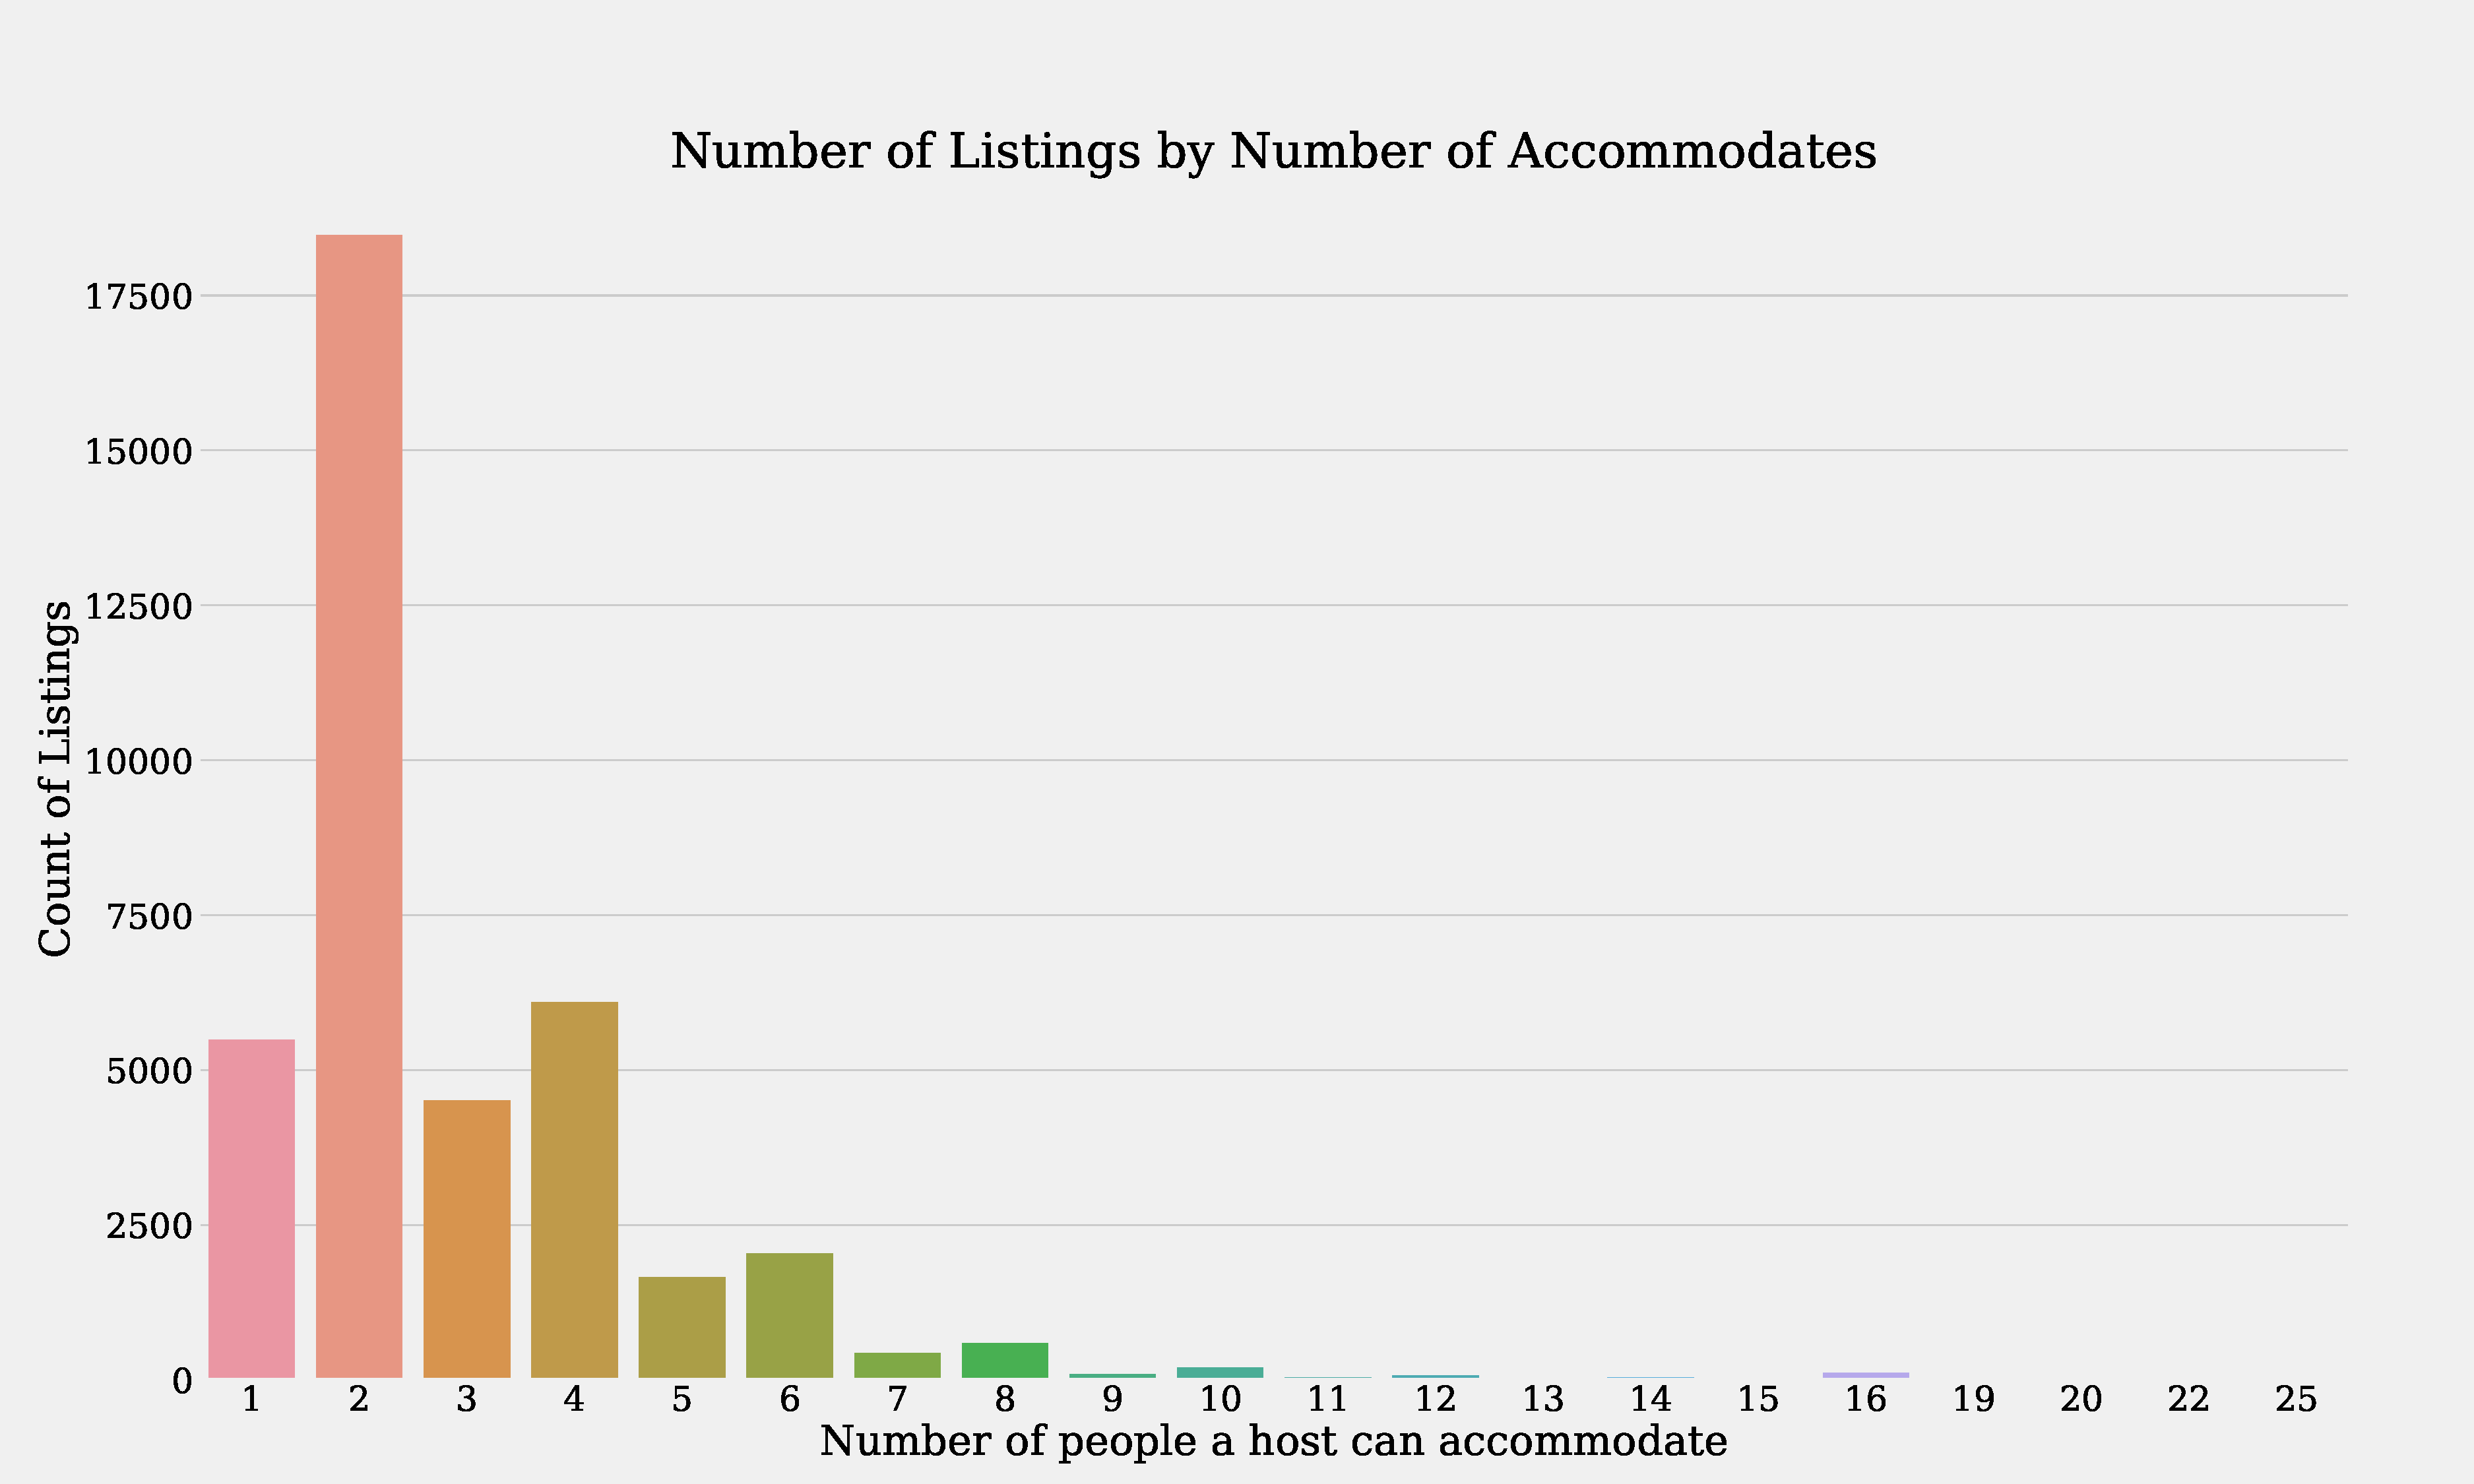
\includegraphics[width=\textwidth]{accommodates-countplot.pdf}
    \caption{Number of Listings by Accomodates}
    \label{fig:accommodates-countplot}
\end{figure}

\begin{figure}[H] \centering
    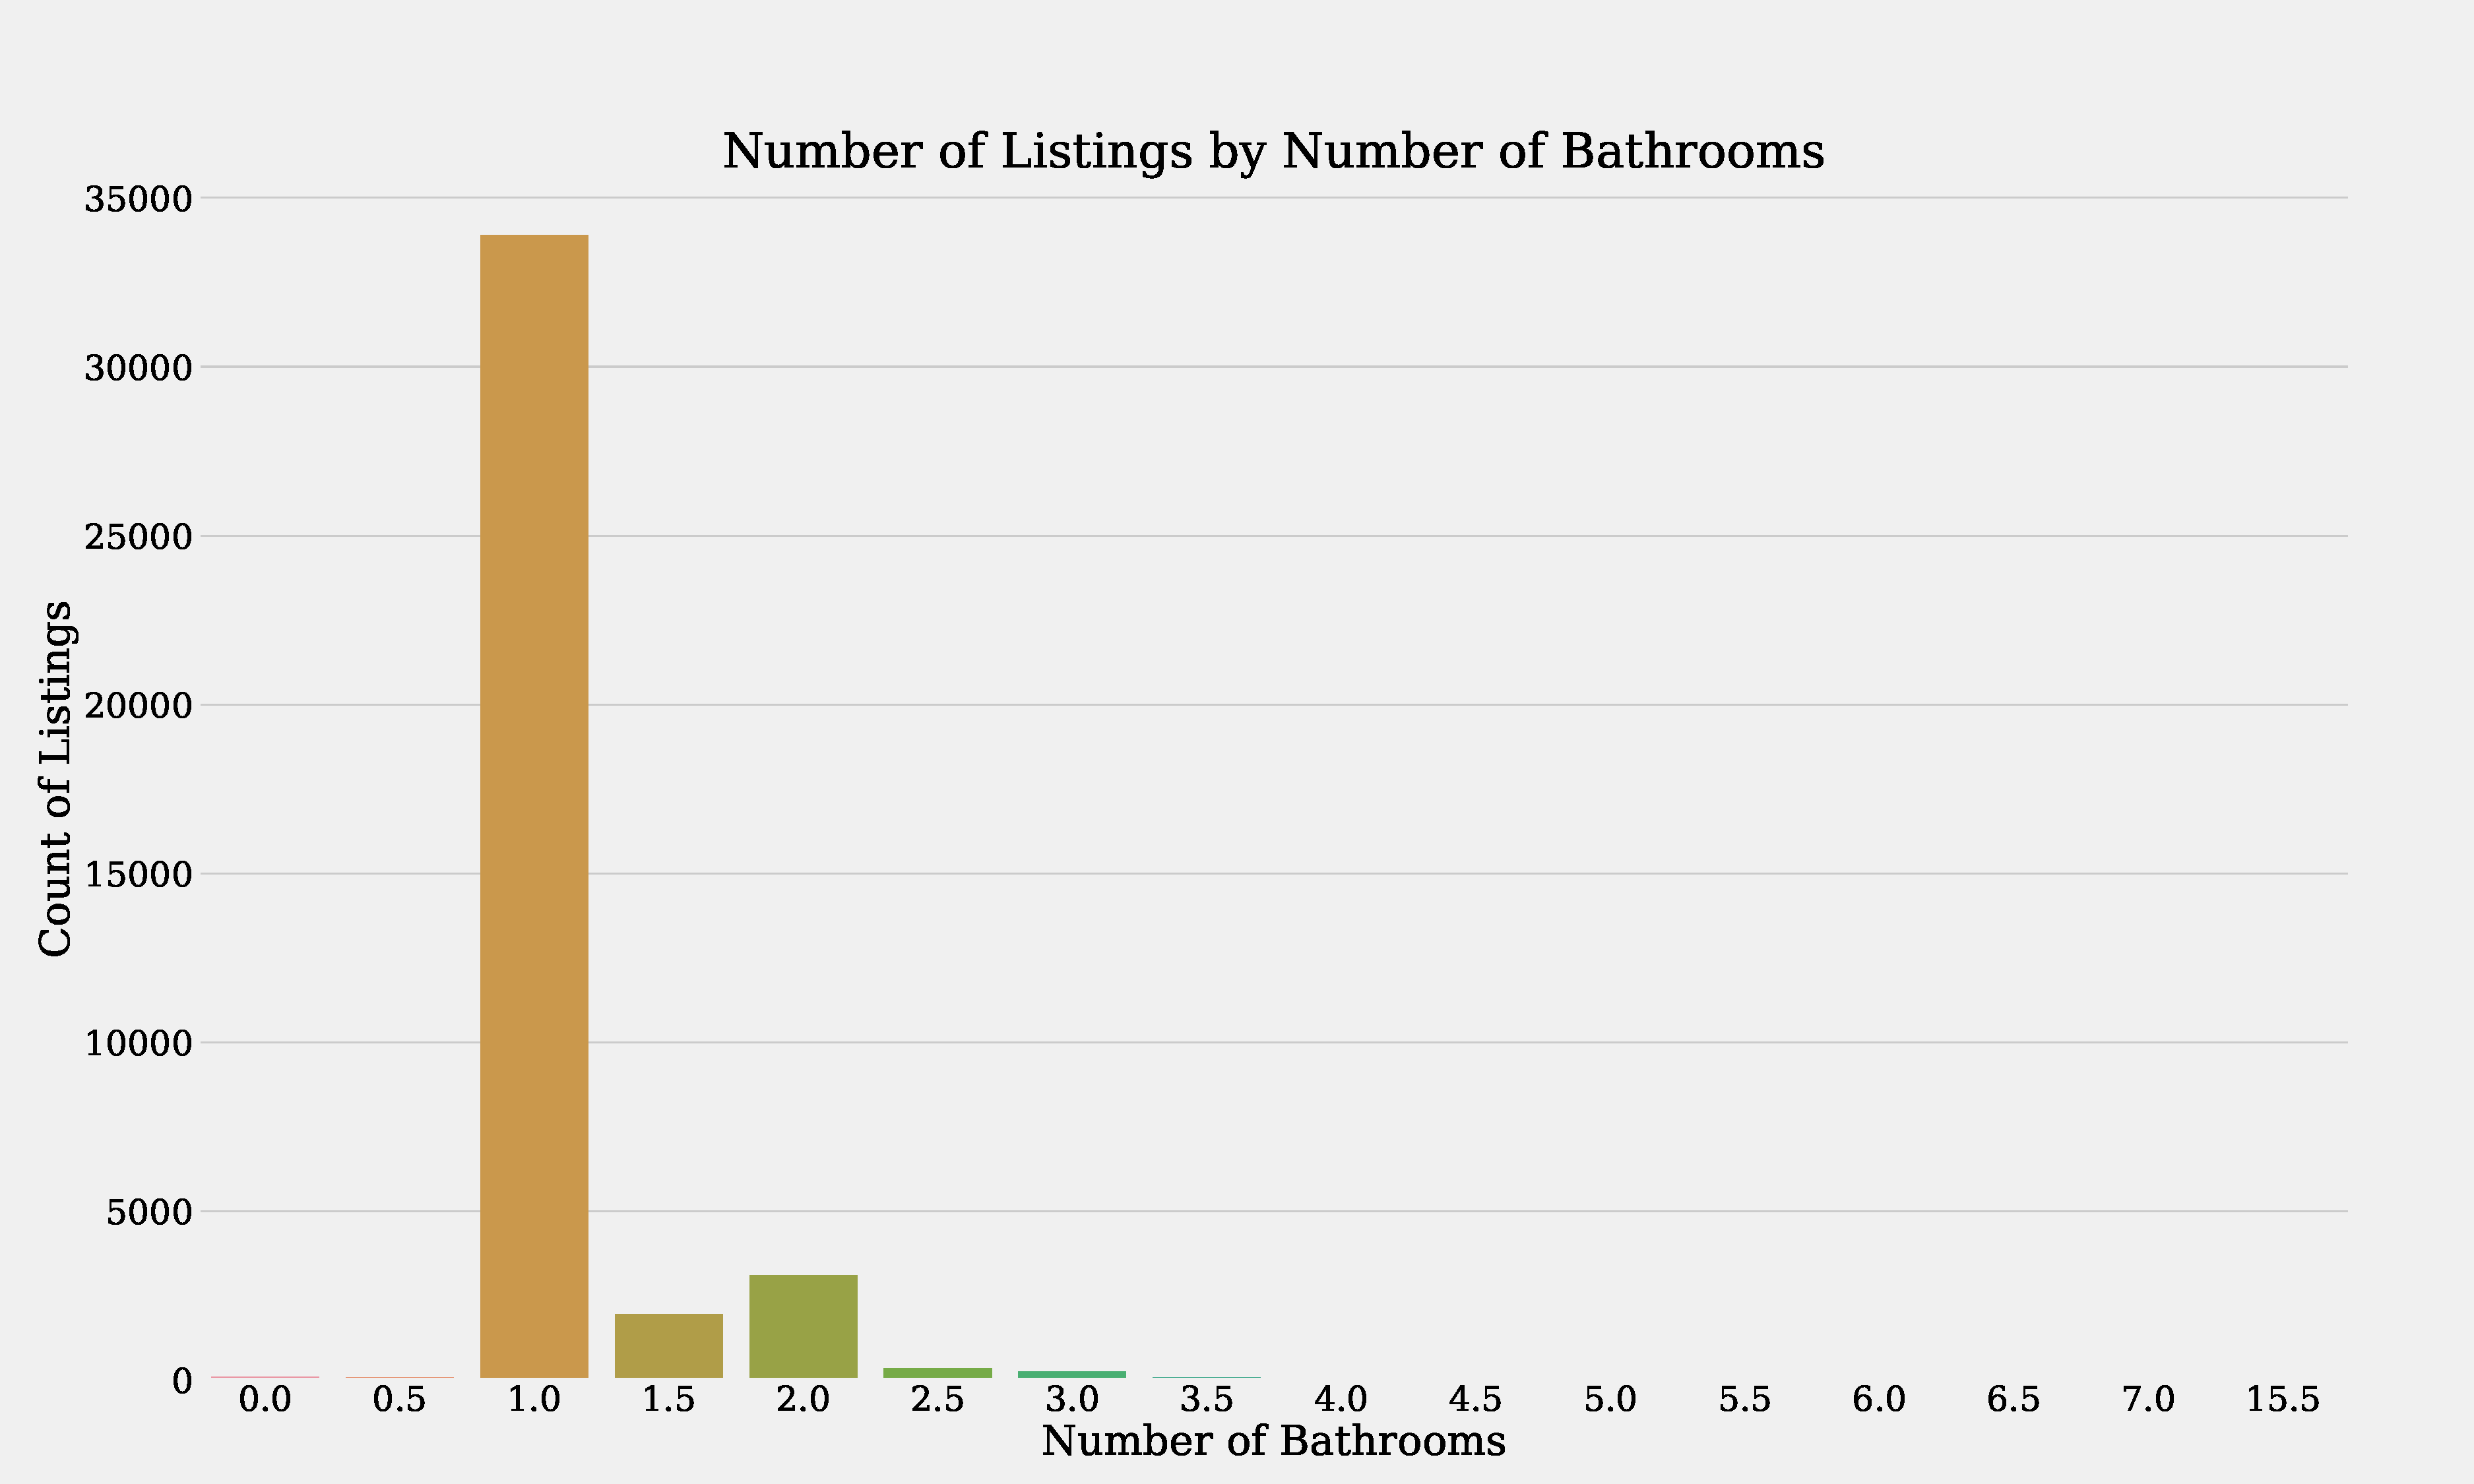
\includegraphics[width=\textwidth]{bathrooms-countplot.pdf}
    \caption{Number of Listings by Number of Bathrooms }
    \label{fig:bathrooms-countplot}
\end{figure}

\begin{figure}[H] \centering
    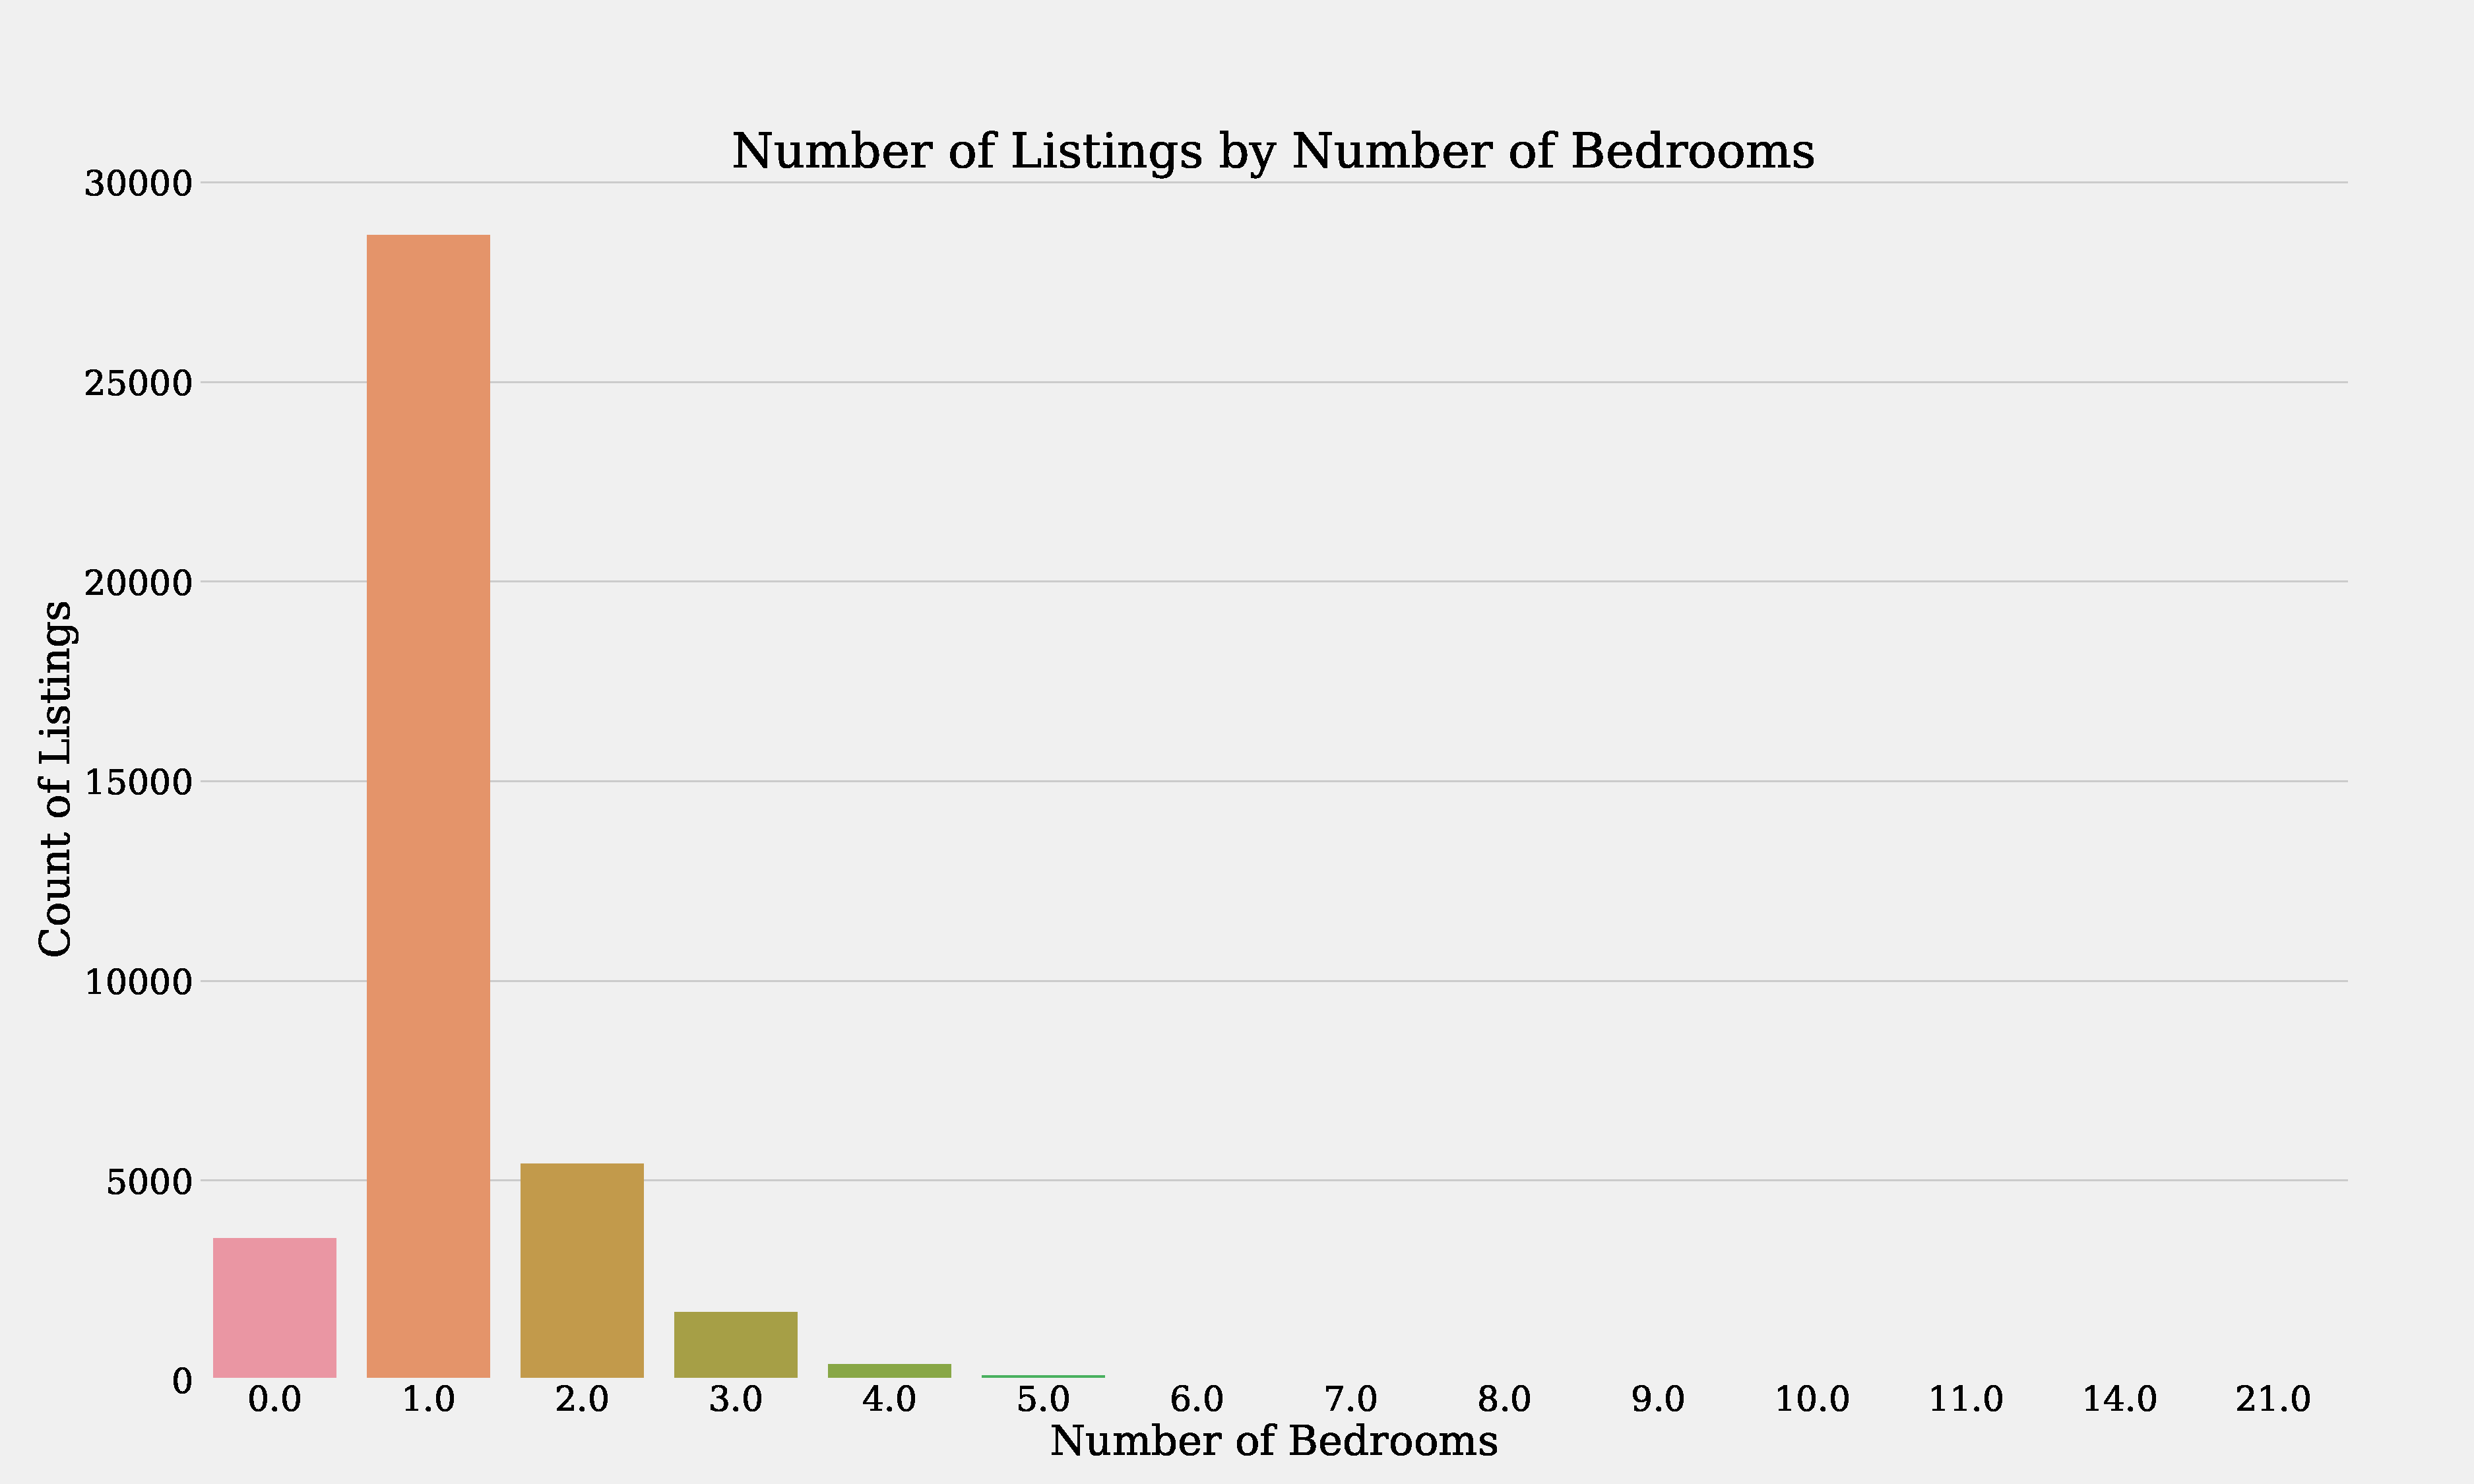
\includegraphics[width=\textwidth]{bedrooms-countplot.pdf}
    \caption{Number of Listings by Number of Bedrooms }
    \label{fig:bedrooms-countplot}
\end{figure}

\begin{figure}[H] \centering
    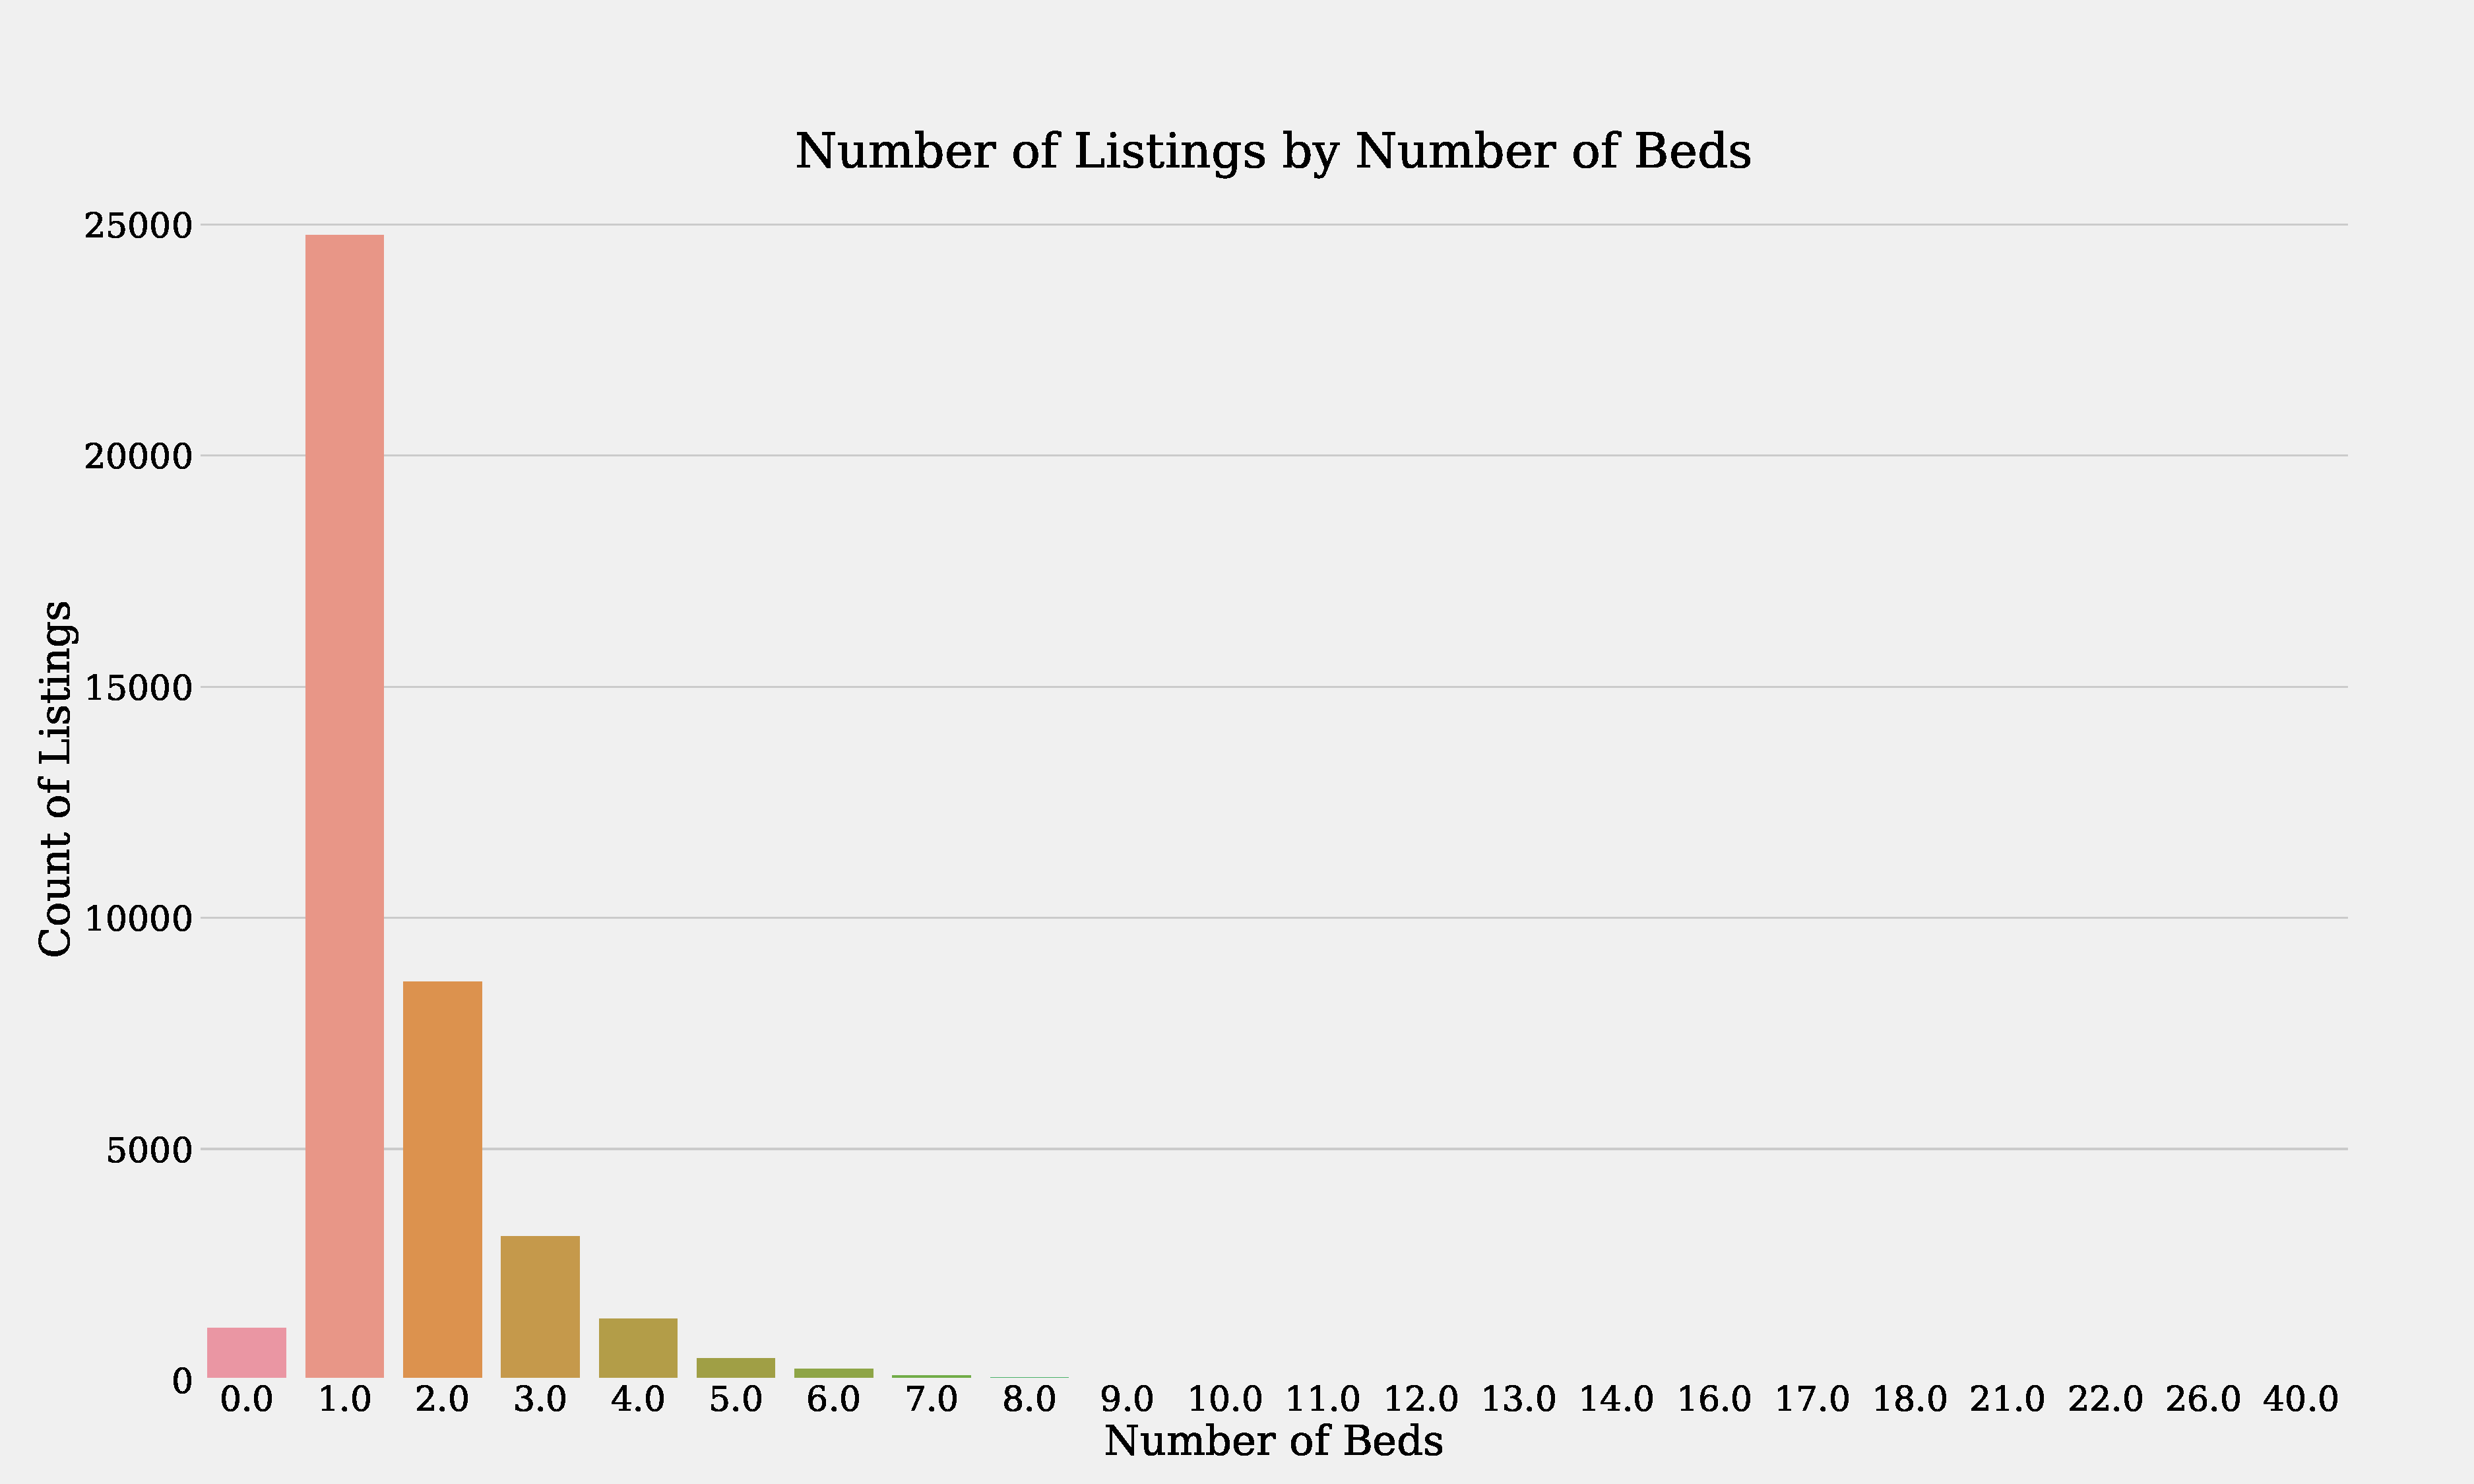
\includegraphics[width=\textwidth]{beds-countplot.pdf}
    \caption{Number of Listings by Number of Beds }
    \label{fig:beds-countplot}
\end{figure}

% ------------------------------
% median price by accommodates, bathrooms, bedrooms, beds
\begin{figure}[H] \centering
    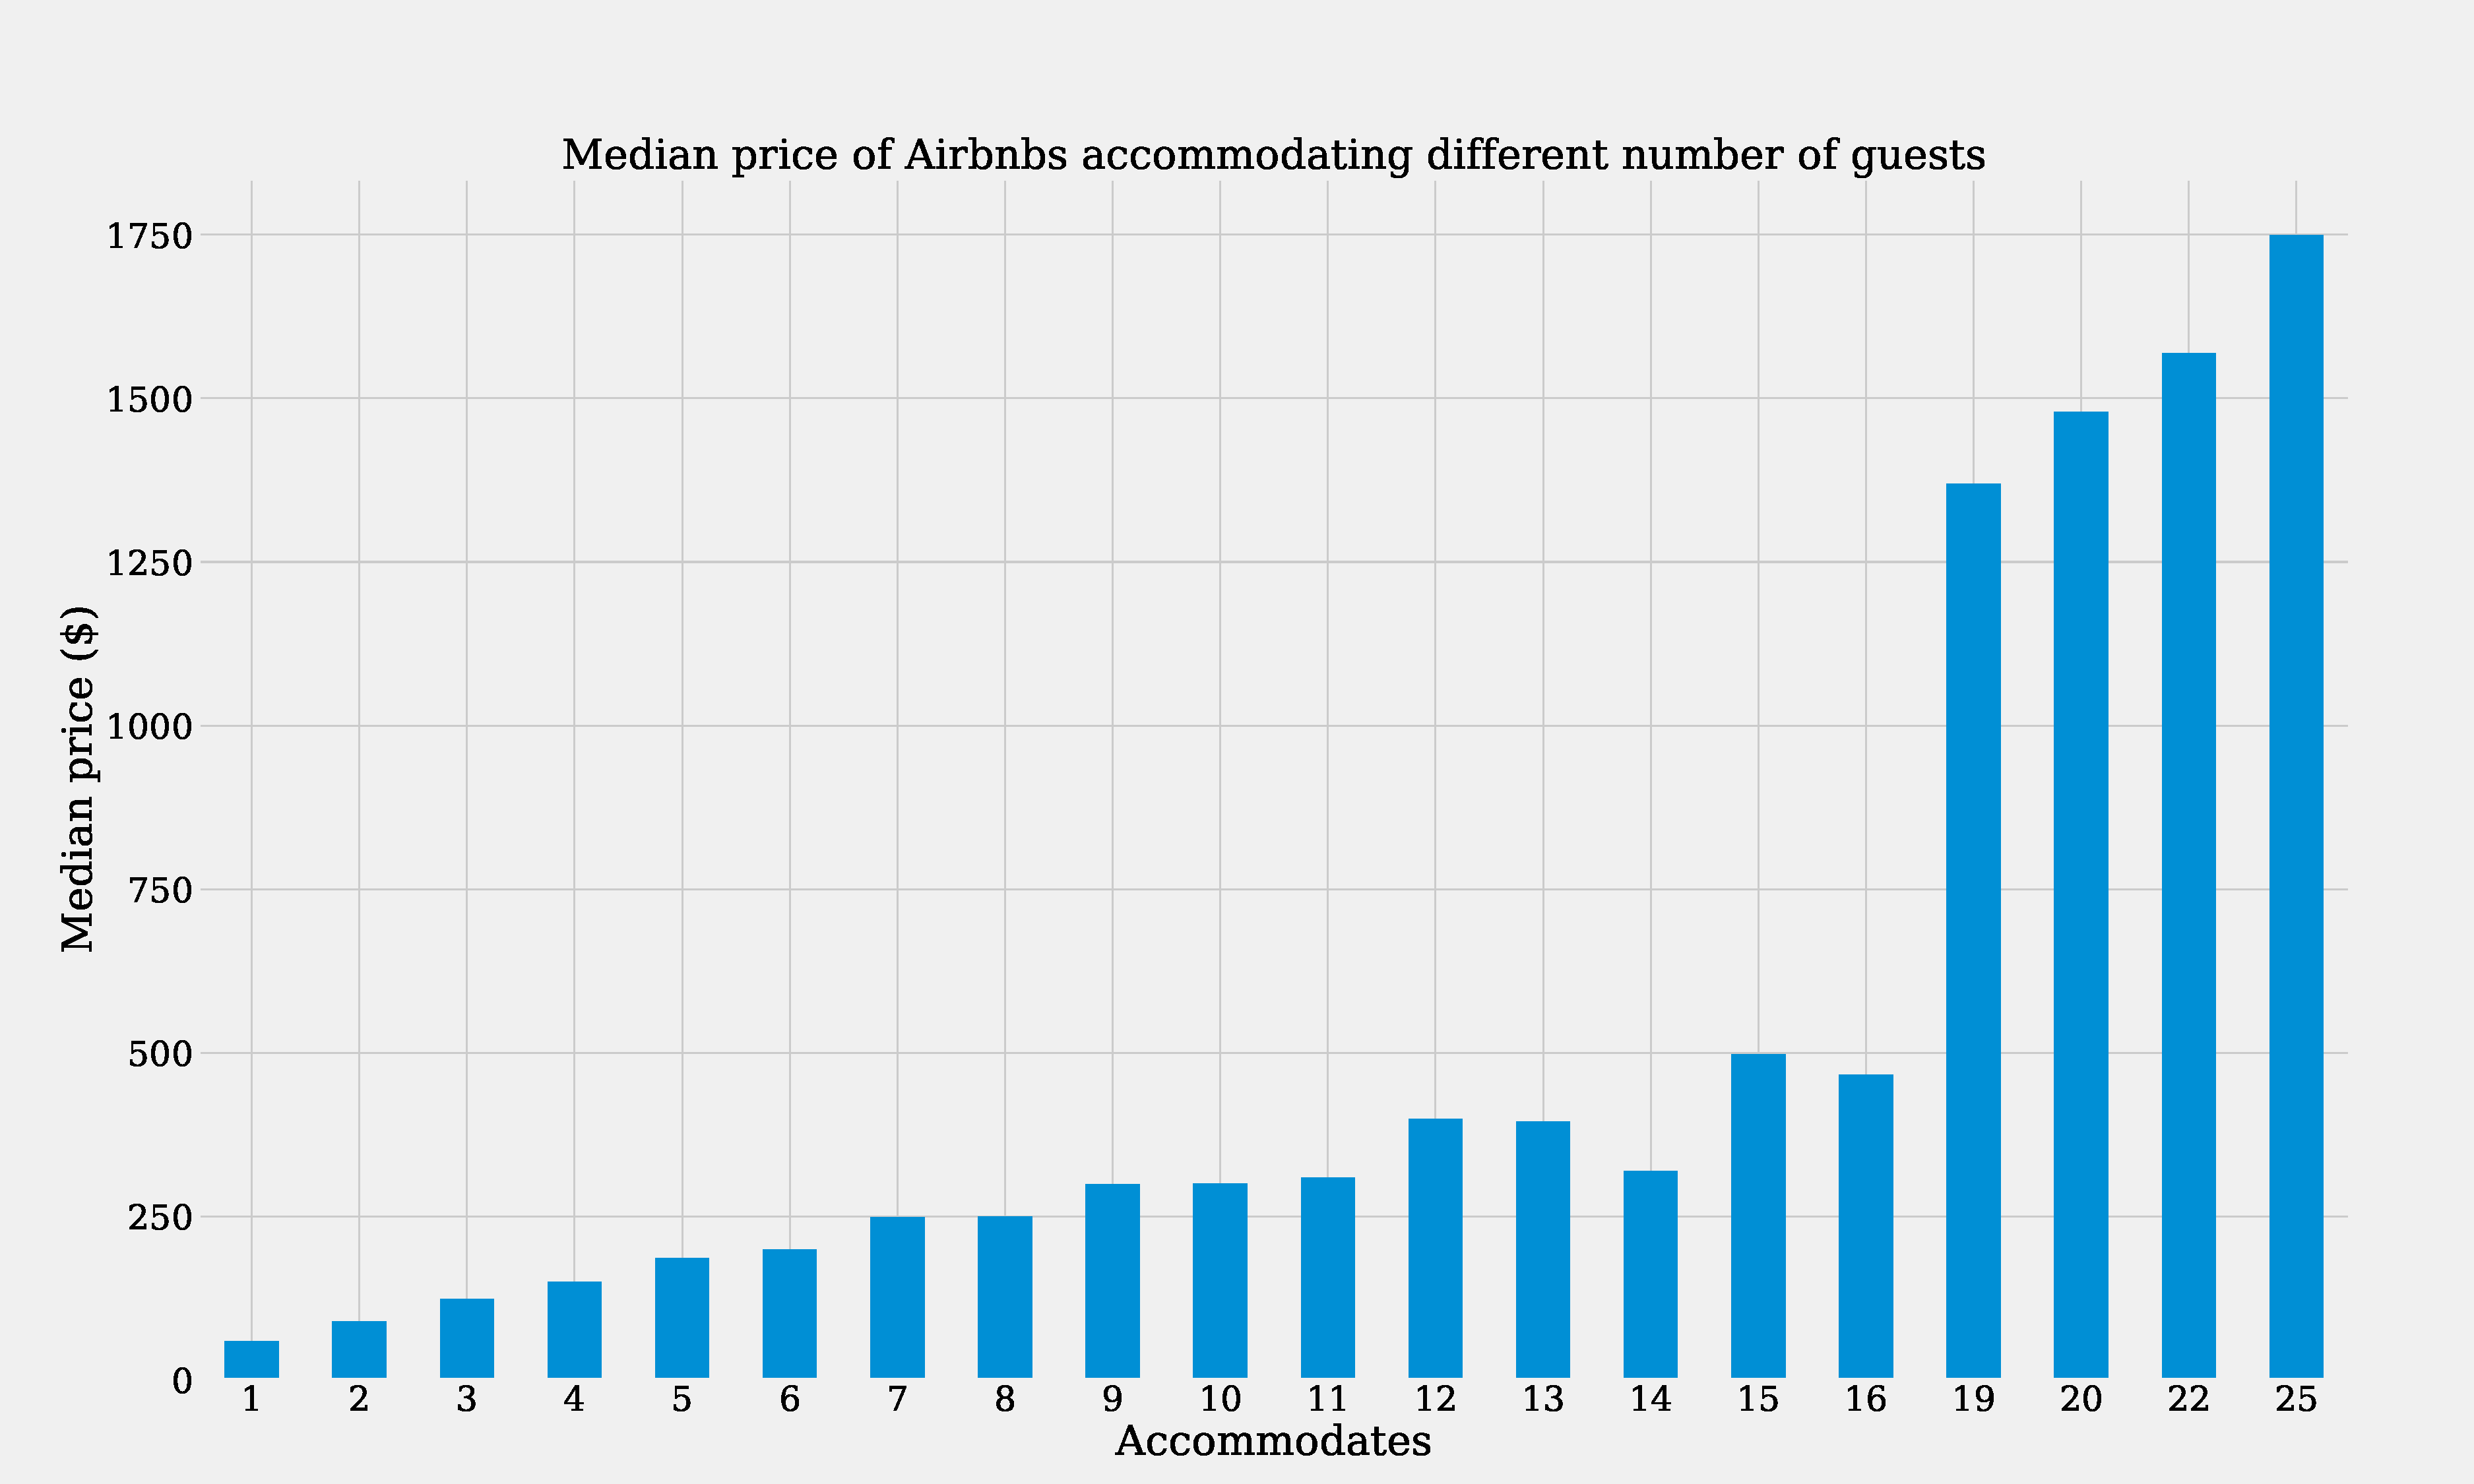
\includegraphics[width=\textwidth]{median-price-by-accommodates.pdf}
    \caption{Median Price By Accommodates}
    \label{fig:median-price-by-accommodates}
\end{figure}

\begin{figure}[H] \centering
    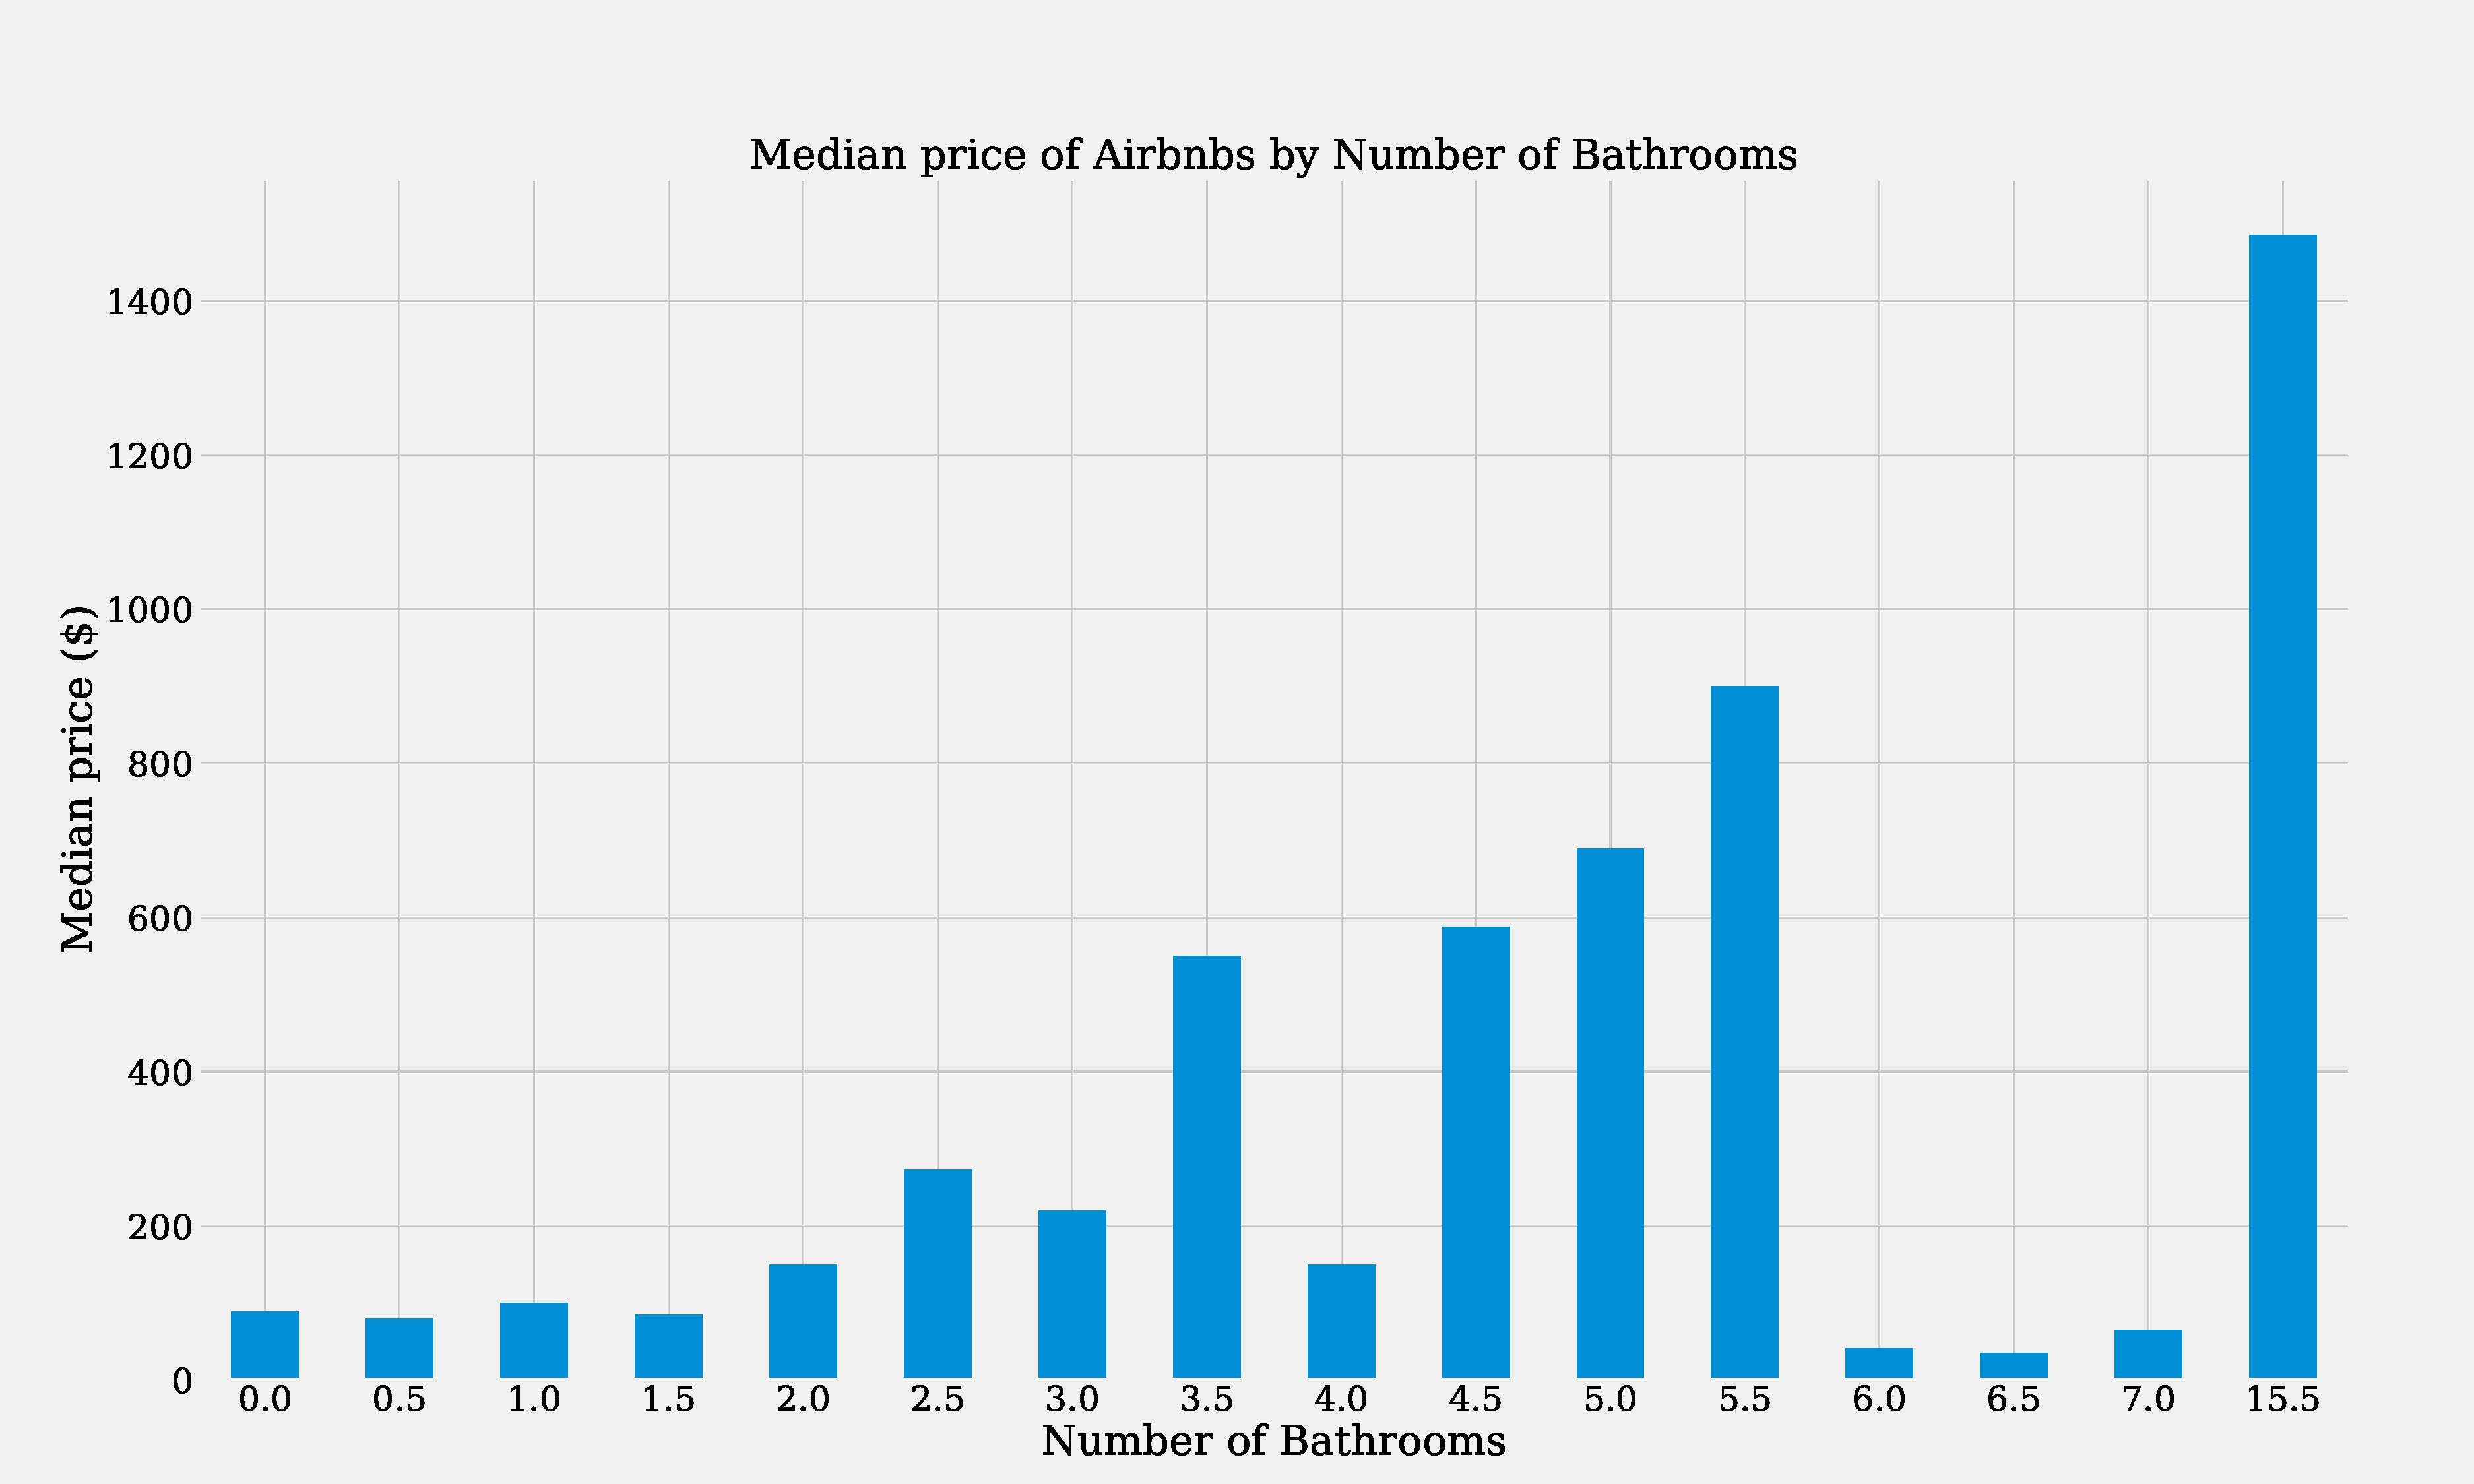
\includegraphics[width=\textwidth]{median-price-by-bathrooms.pdf}
    \caption{Median Price By  Number of Bathrooms }
    \label{fig:median-price-by-bathrooms}
\end{figure}

\begin{figure}[H] \centering
    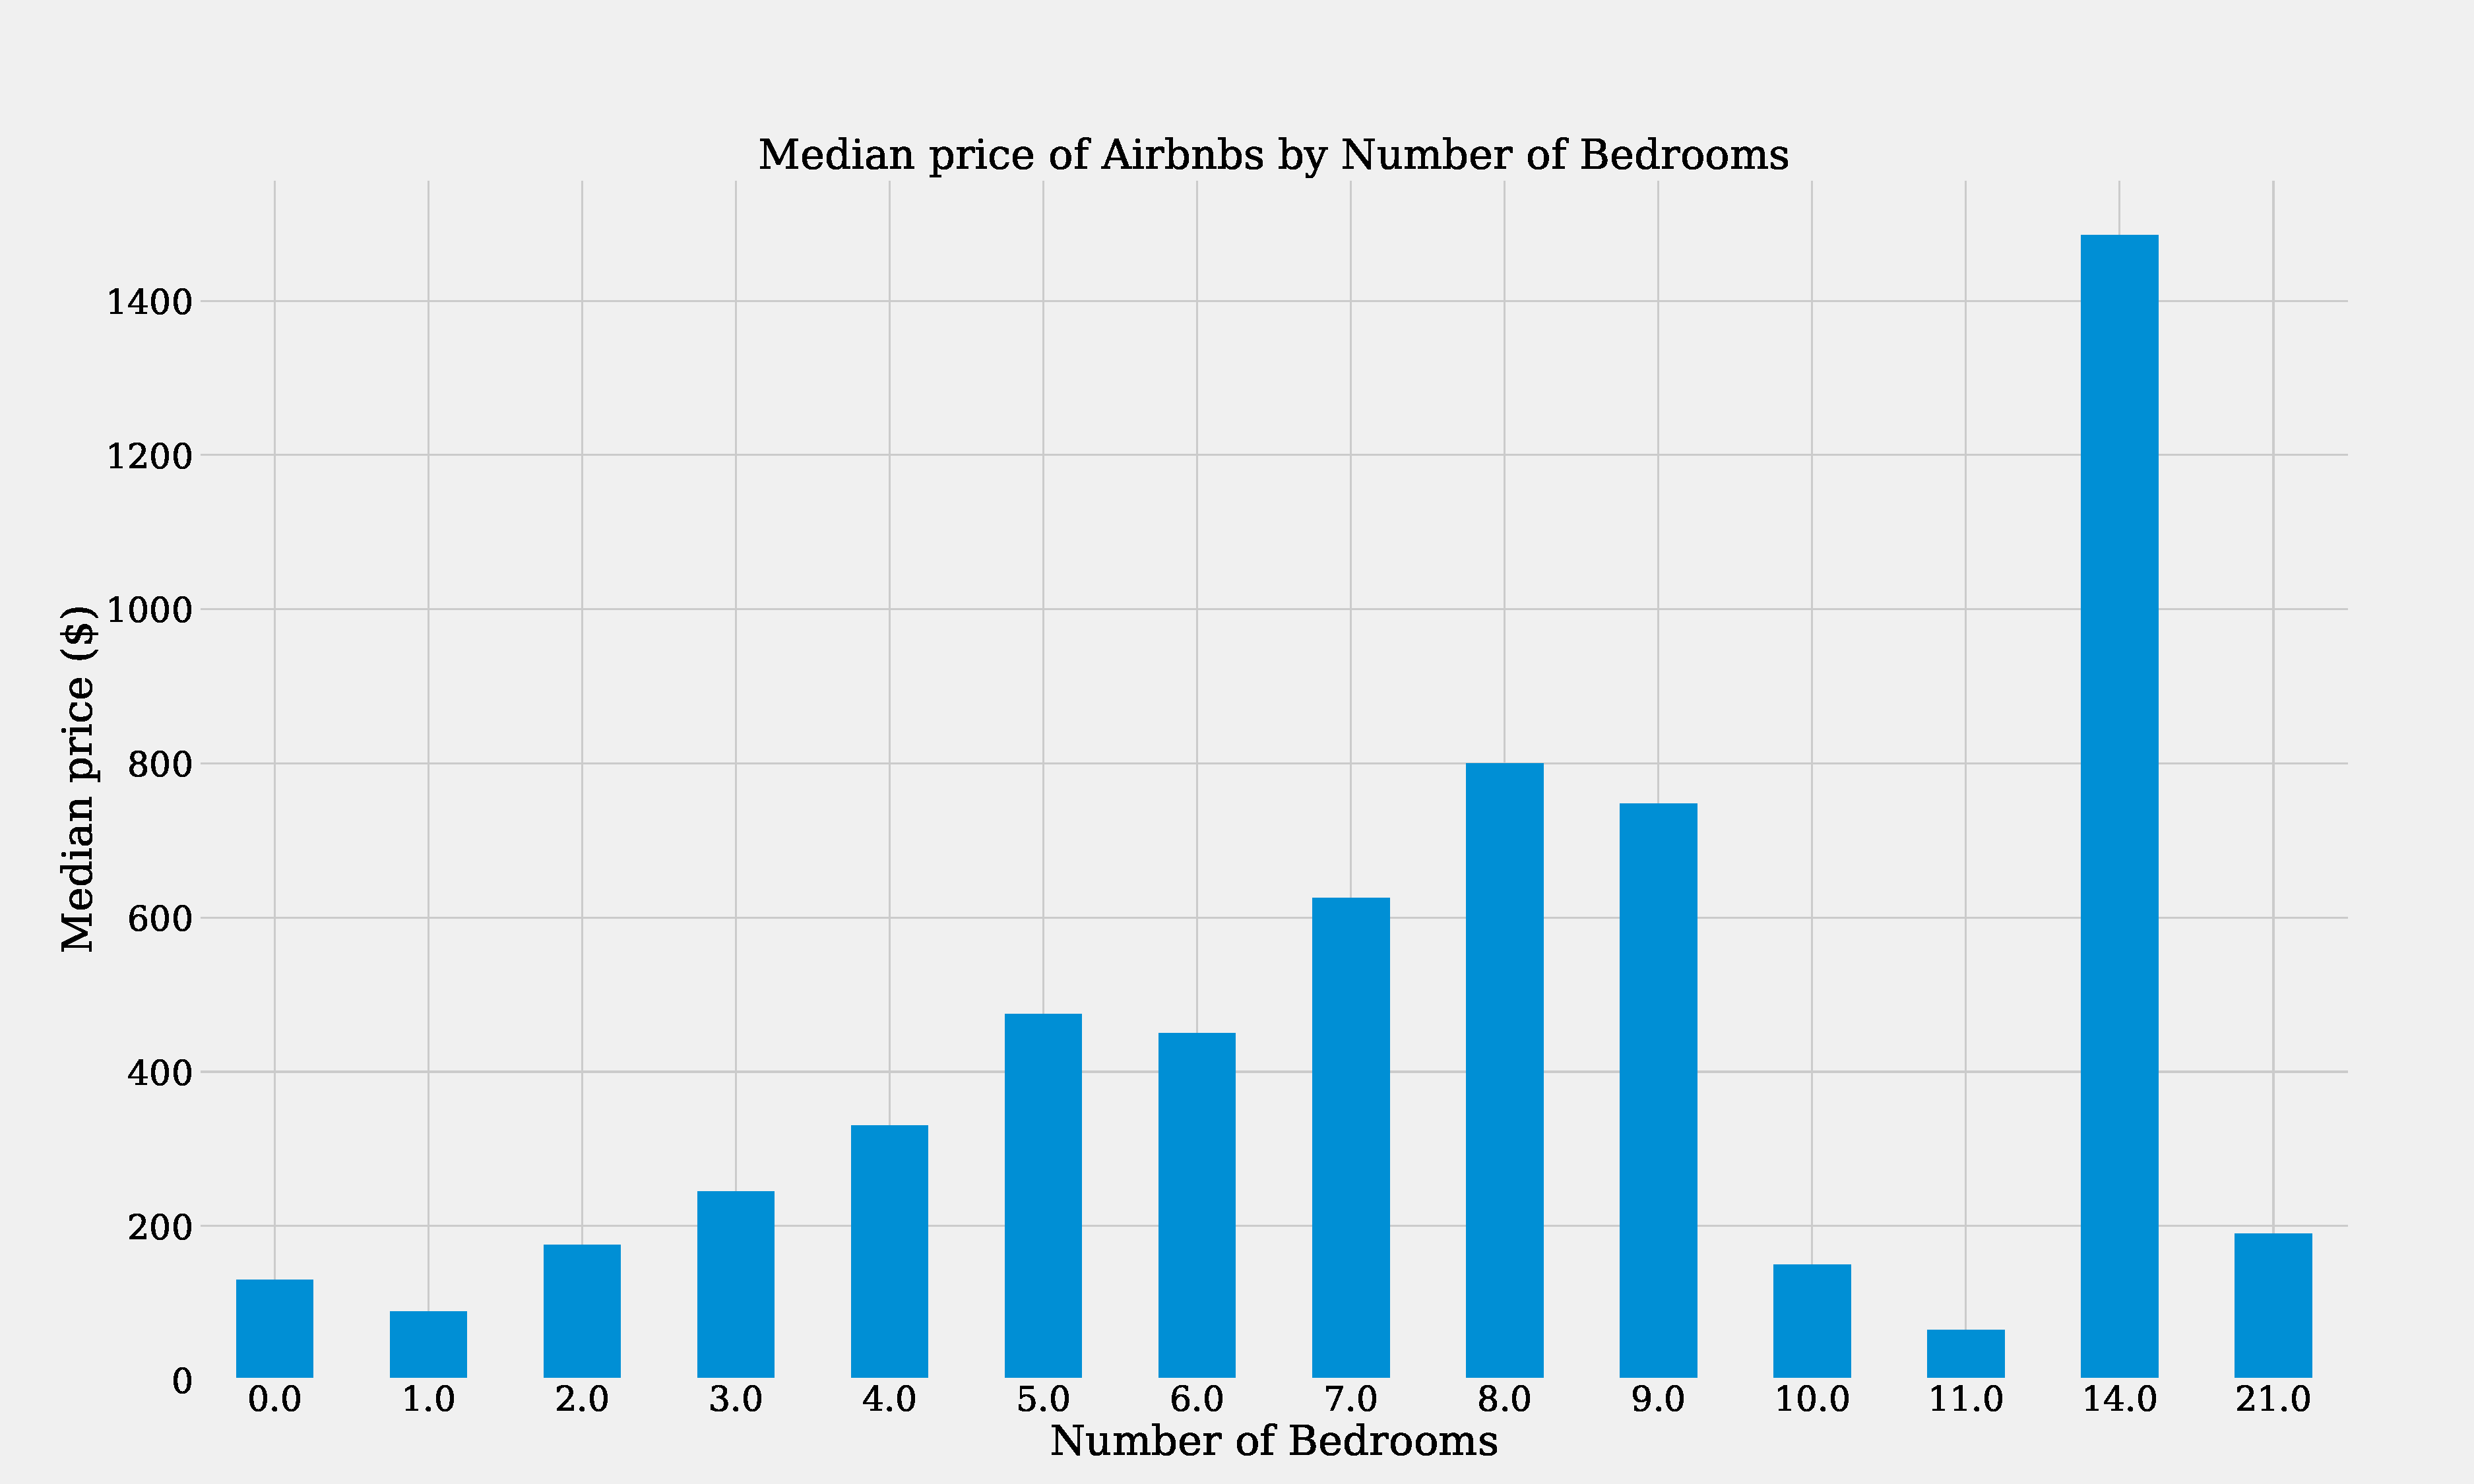
\includegraphics[width=\textwidth]{median-price-by-bedrooms.pdf}
    \caption{Median Price By Number of Bedrooms}
    \label{fig:median-price-by-bedrooms}
\end{figure}


\begin{figure}[H] \centering
    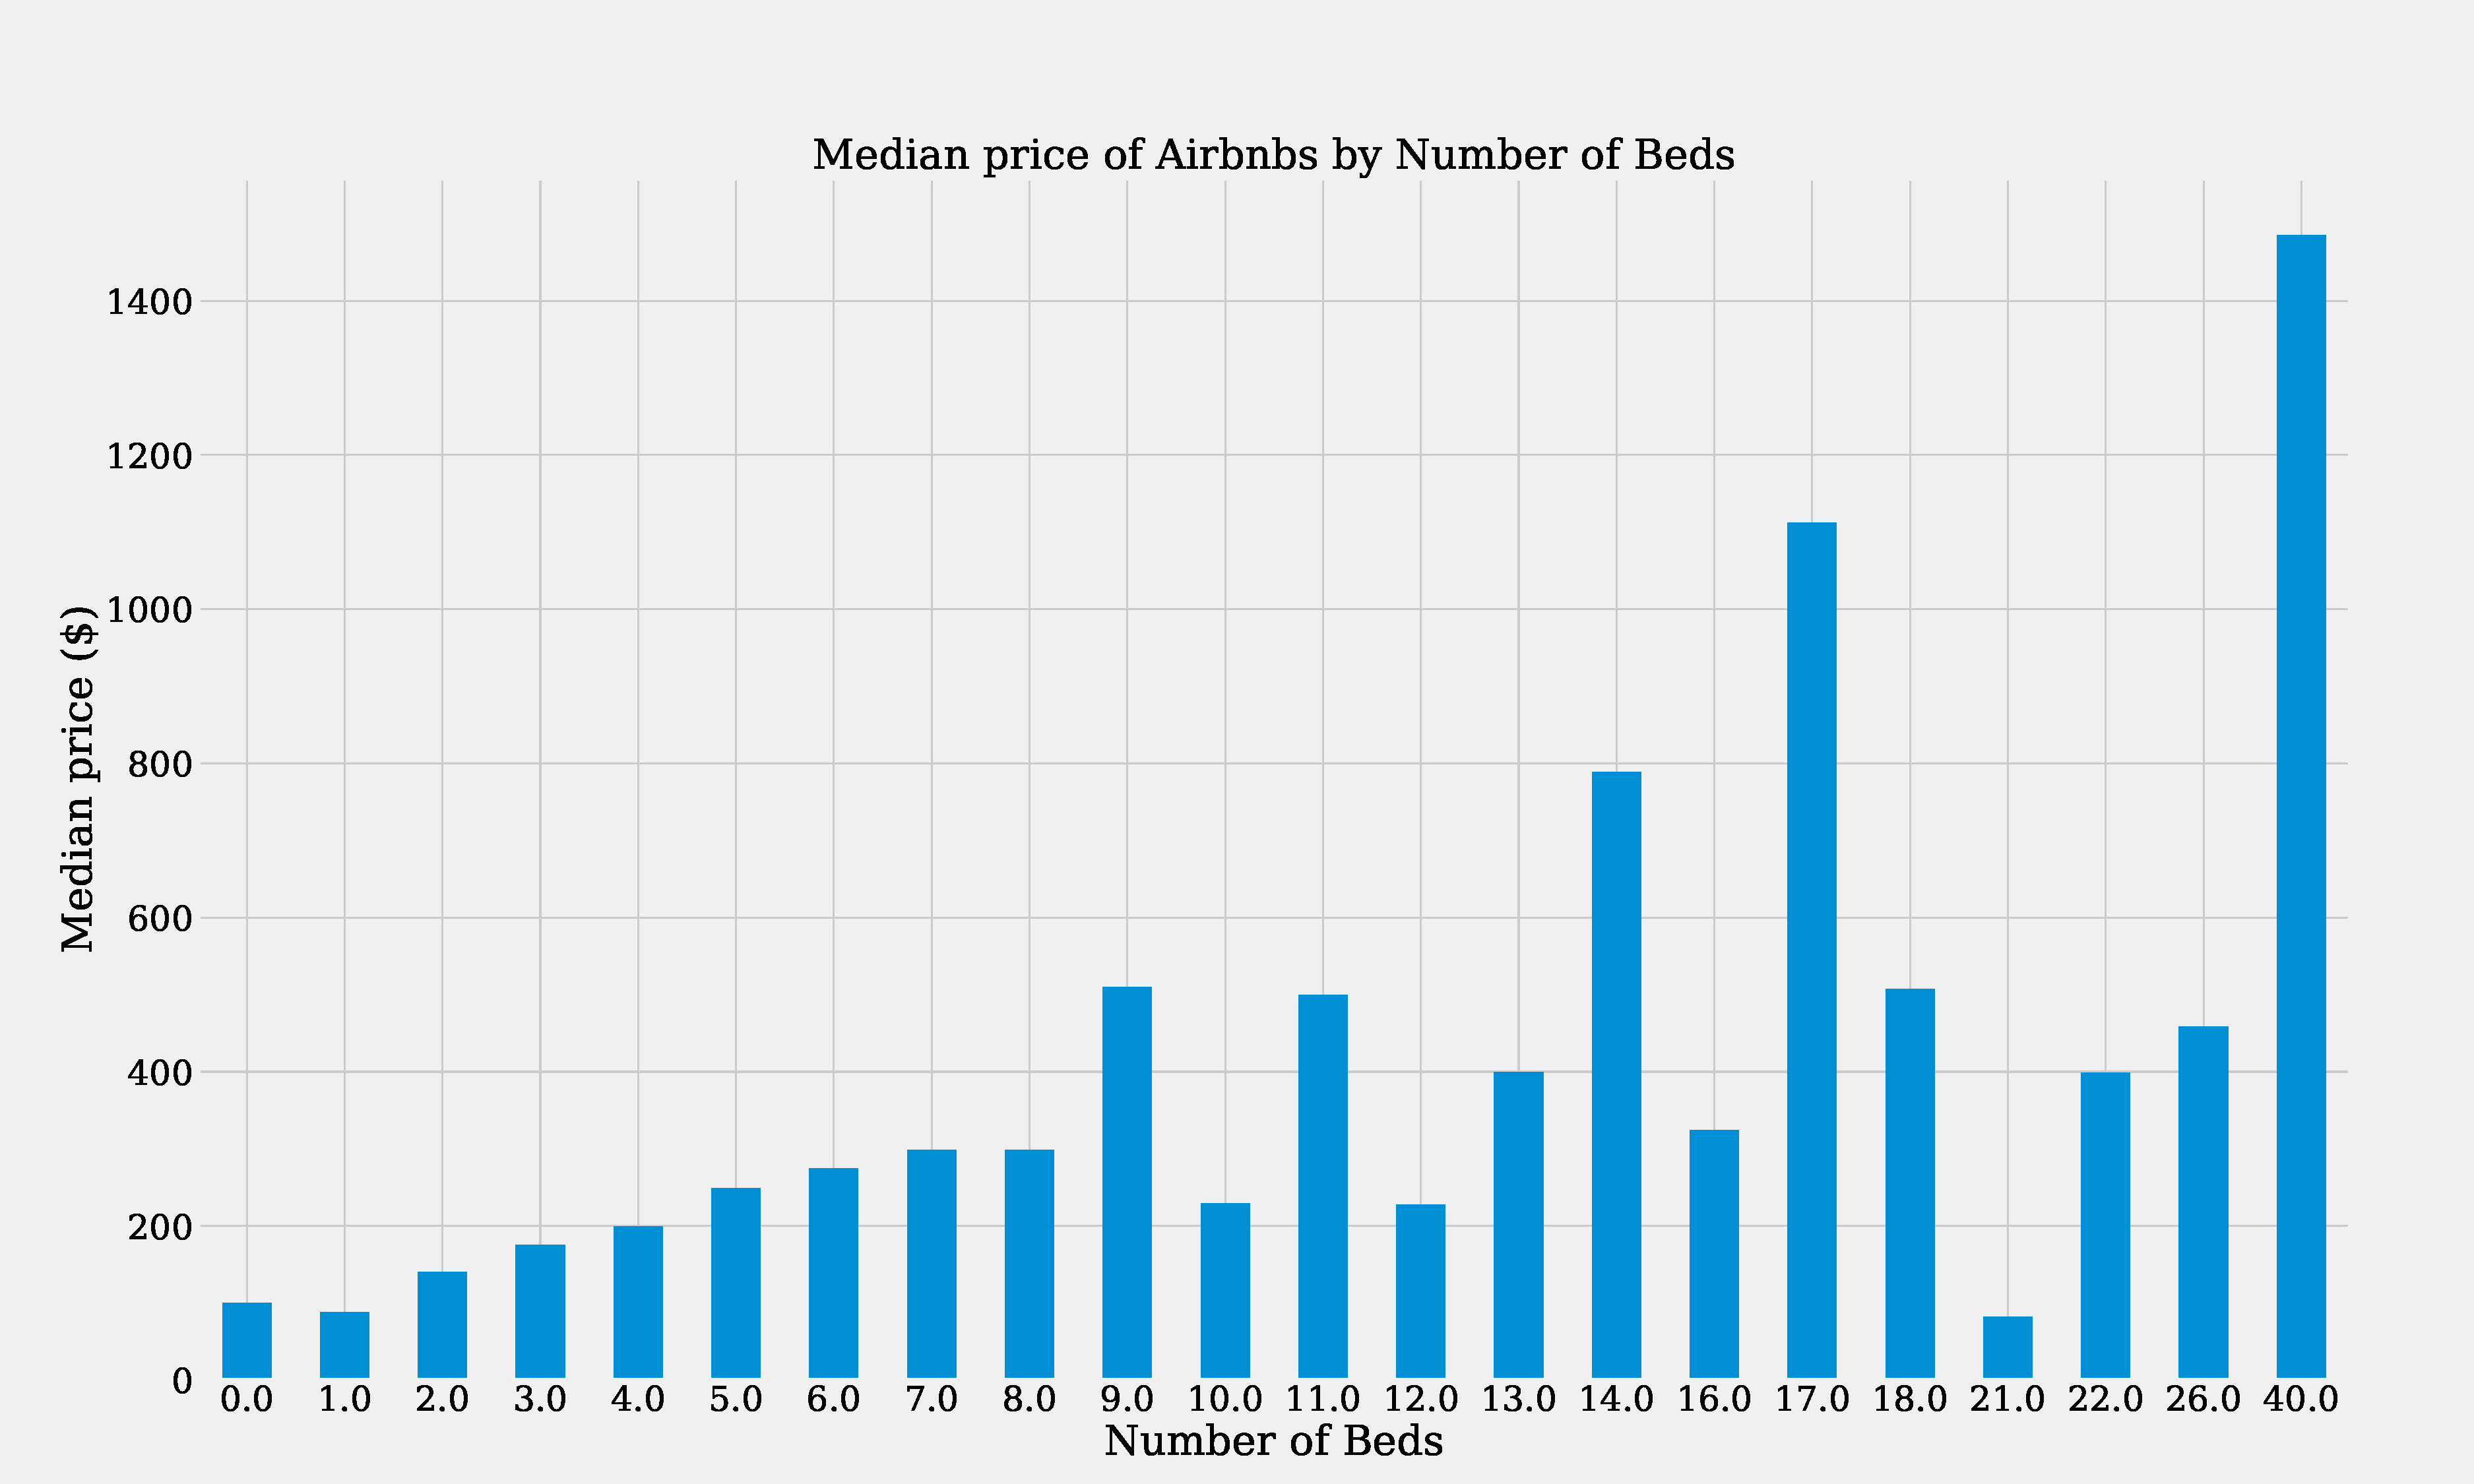
\includegraphics[width=\textwidth]{median-price-by-beds.pdf}
    \caption{Median Price By Number of Beds}
    \label{fig:median-price-by-beds}
\end{figure}

% ------------------------------

% Amenity Group 1
\begin{figure}[H]
\centering
    \caption{Elevator and Bed Linen}
    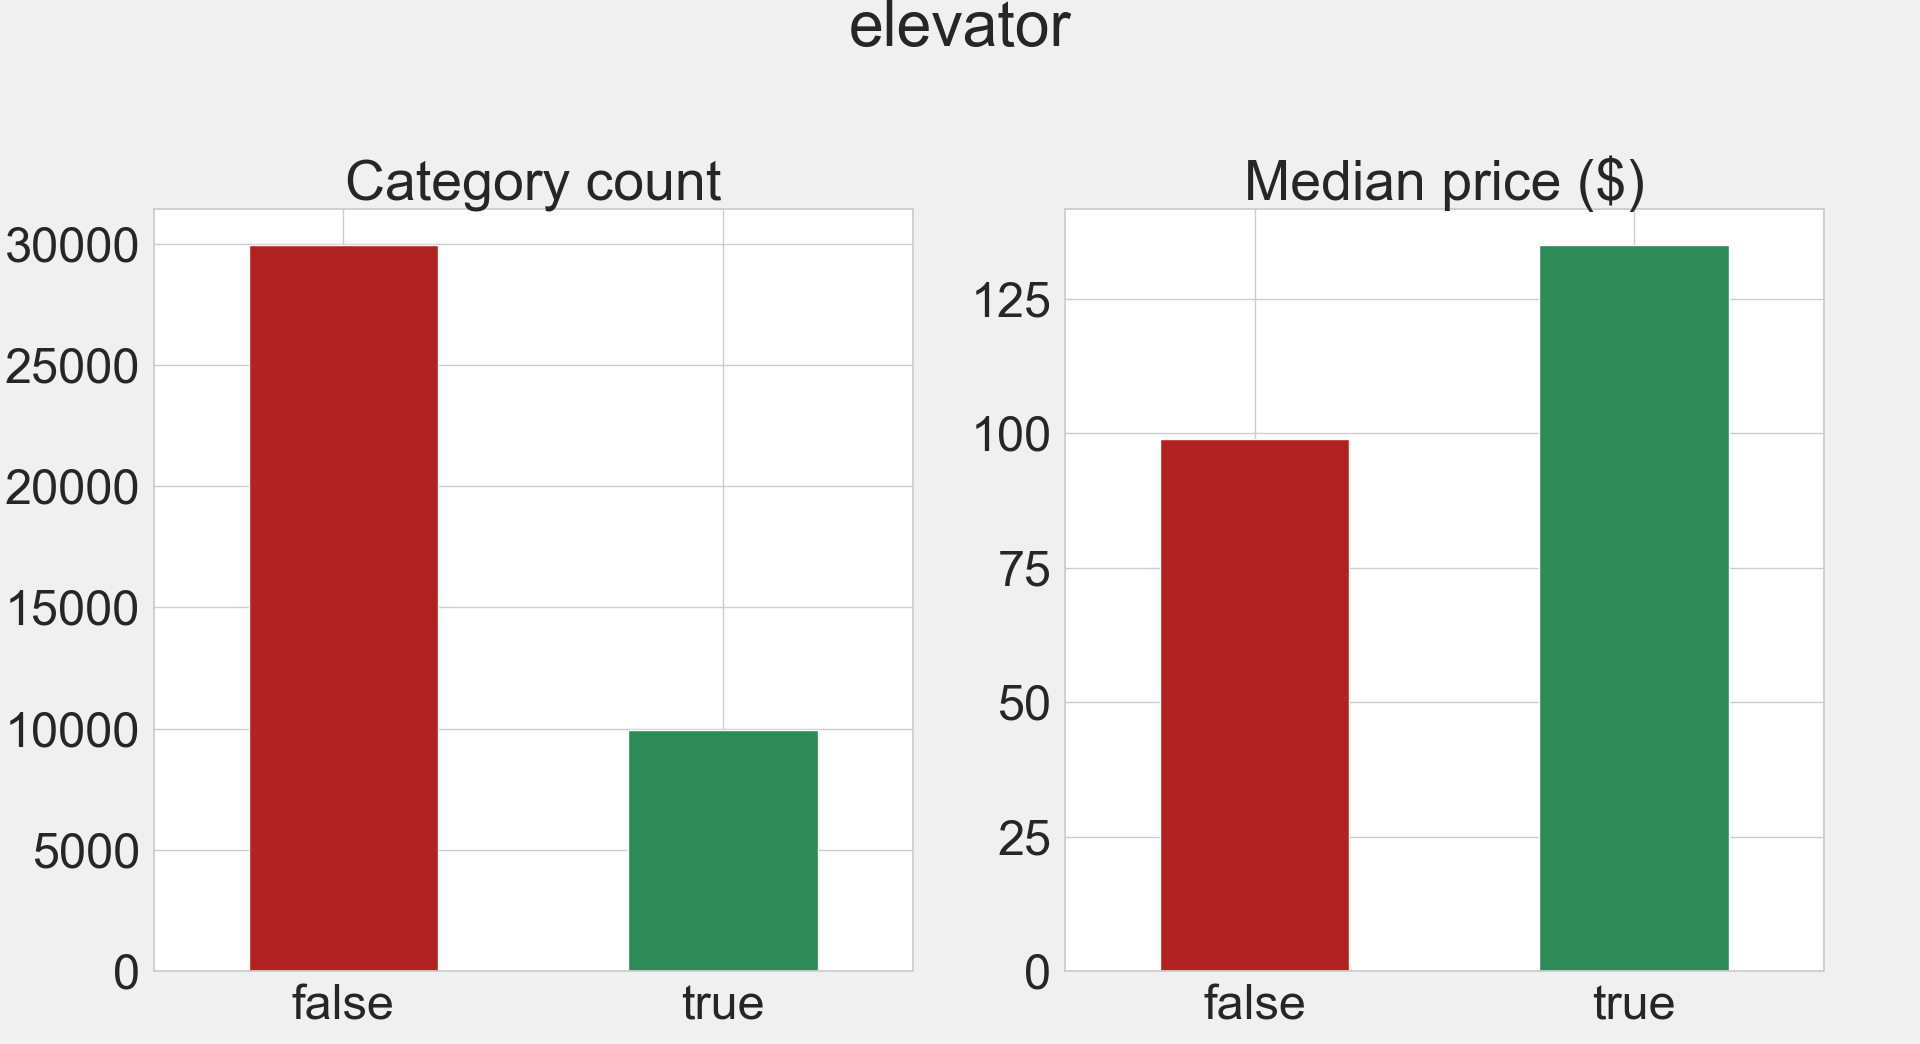
\includegraphics[width=\linewidth]{figures/amenities/group1/elevator.png}
    %\caption{Caption 1}
    \vspace{0.3cm}
    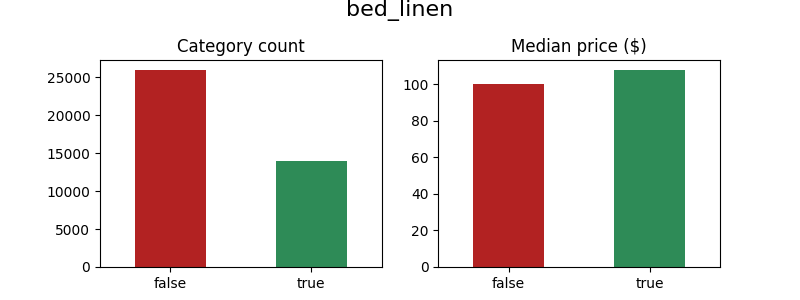
\includegraphics[width=\linewidth]{figures/amenities/group1/bed_linen.png}
    %\caption{Caption 2}
    \label{fig:elevator-and-bed-linen}
\end{figure}


\begin{figure}[H]
\centering
\caption{White Goods and Pets Allowed}
    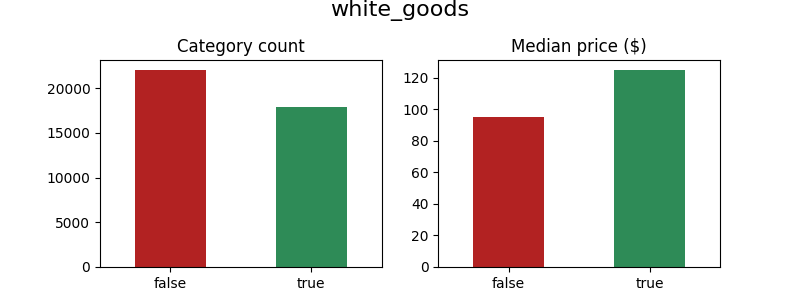
\includegraphics[width=\linewidth]{figures/amenities/group1/white_goods.png}
    %\caption{Caption 1}
    \vspace{0.5cm}
    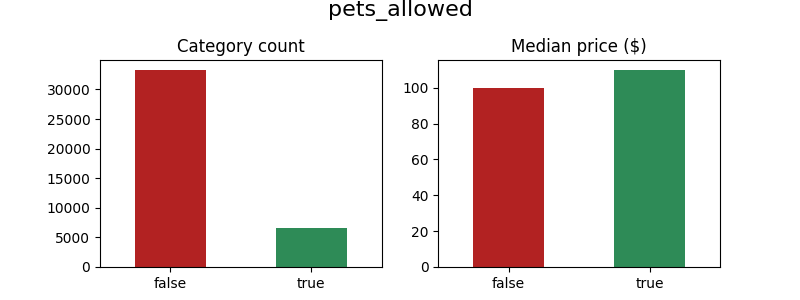
\includegraphics[width=\linewidth]{figures/amenities/group1/pets_allowed.png}
    %\caption{Caption 2}
    \label{fig:white-goods-and-pets-allowed}
    \
\end{figure}

\begin{figure}[H]
\centering
\caption{Self Check In and Coffee Machine}
    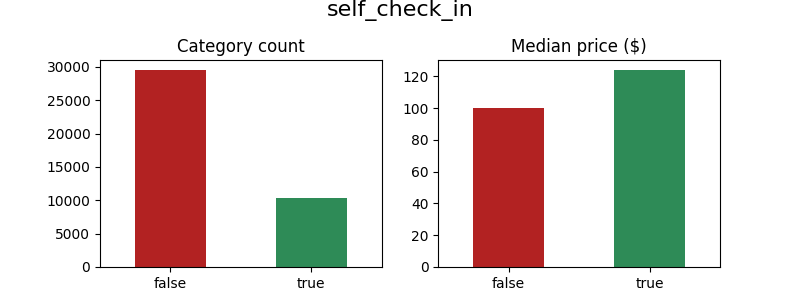
\includegraphics[width=\linewidth]{figures/amenities/group1/self_checkin.png}
    %\caption{Caption 1}
    \vspace{0.5cm}
    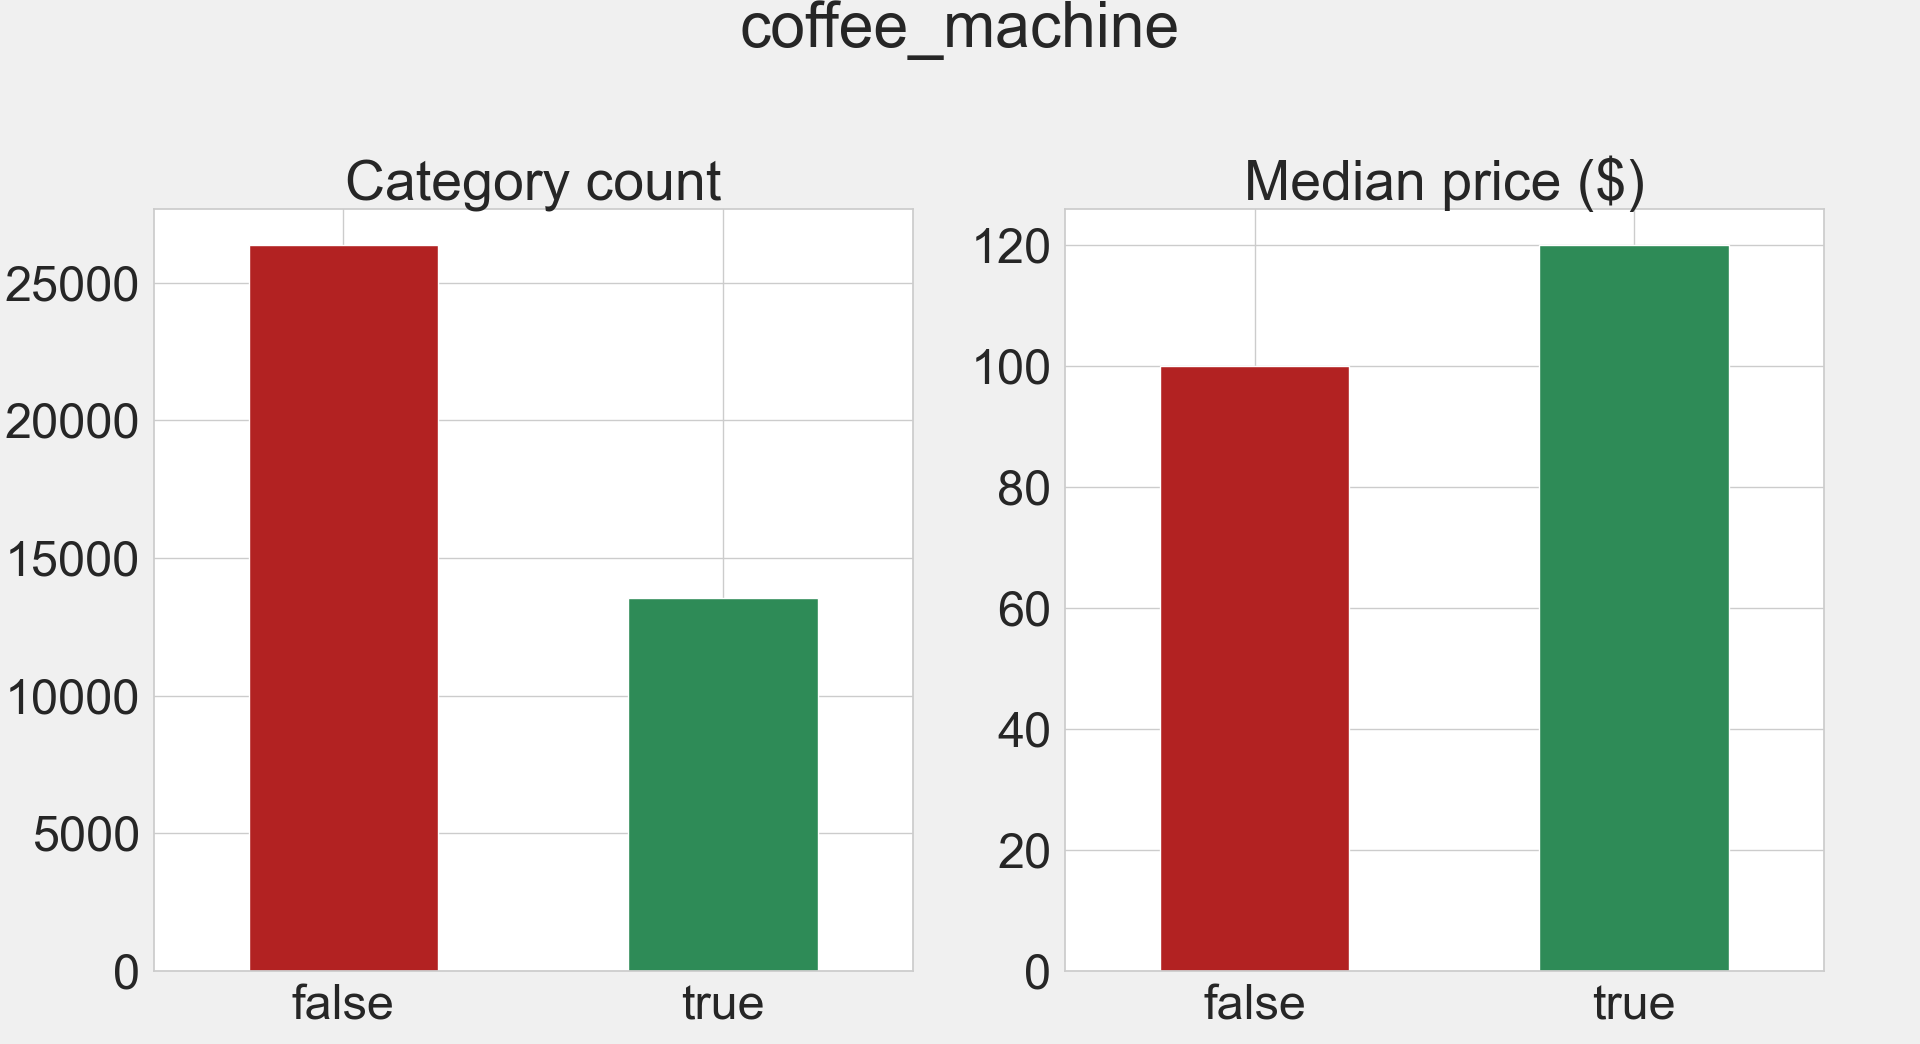
\includegraphics[width=\linewidth]{figures/amenities/group1/coffee_machine.png}
    %\caption{Caption 2}
    \label{fig:self-checkin-and-coffee-machine}
\end{figure}

\begin{figure}[H]
    \centering
    \caption{Long Term Stays and Child Friendly}
    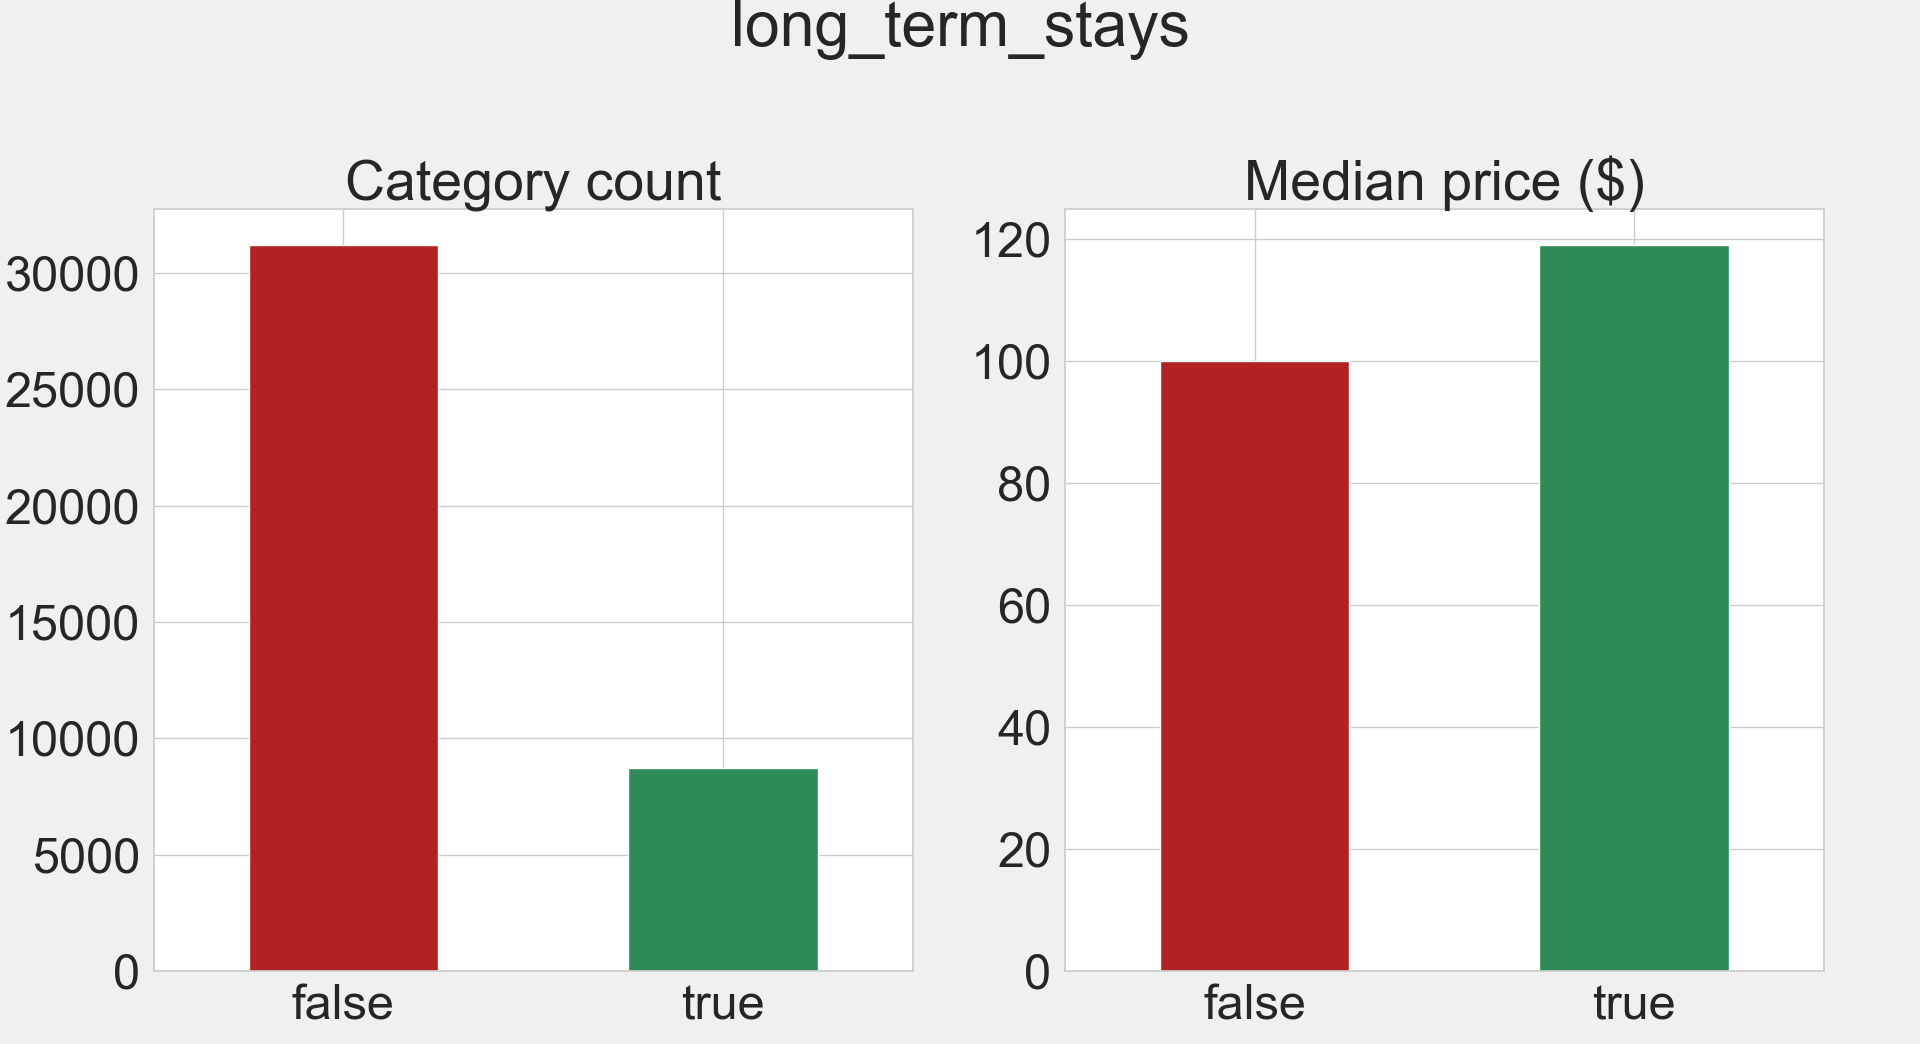
\includegraphics[width=\linewidth]{figures/amenities/group1/long_term_stays.png}
    %\caption{Caption 1}
    \vspace{0.5cm}
    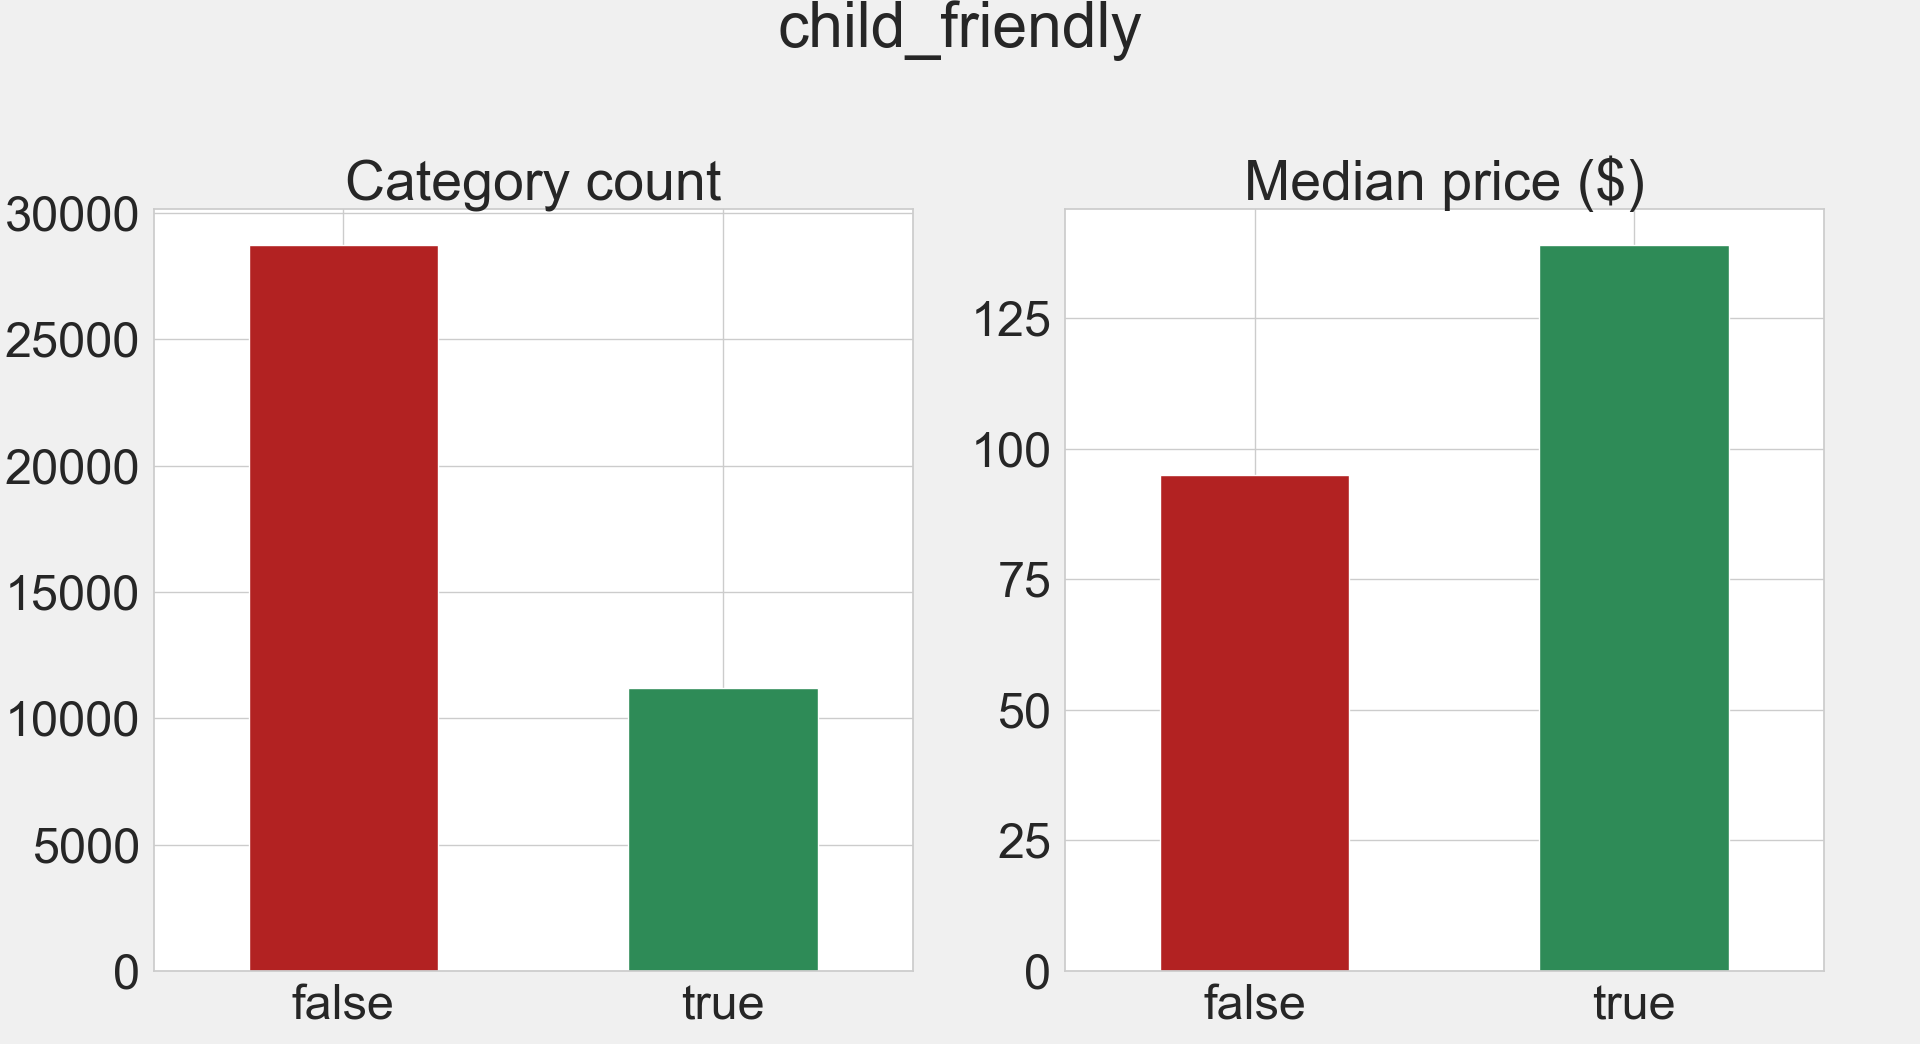
\includegraphics[width=\linewidth]{figures/amenities/group1/child_friendly.png}
    %\caption{Caption 2}
    \label{fig:long-term-stays-and-child-friendly}
\end{figure}

\begin{figure}[H]
\centering
\caption{Private Entrance and Cooking Basics}
    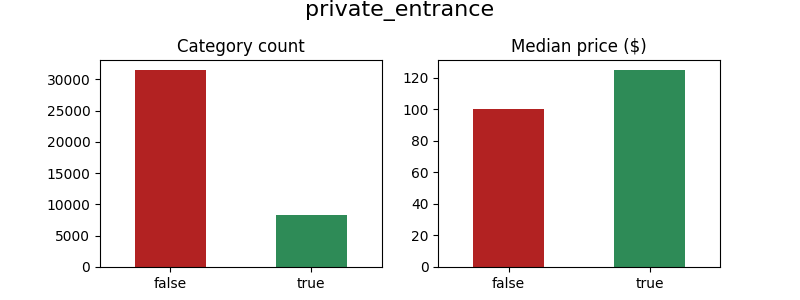
\includegraphics[width=\linewidth]{figures/amenities/group1/private_entrance.png}
    %\caption{Caption 1}
    \vspace{0.5cm}
    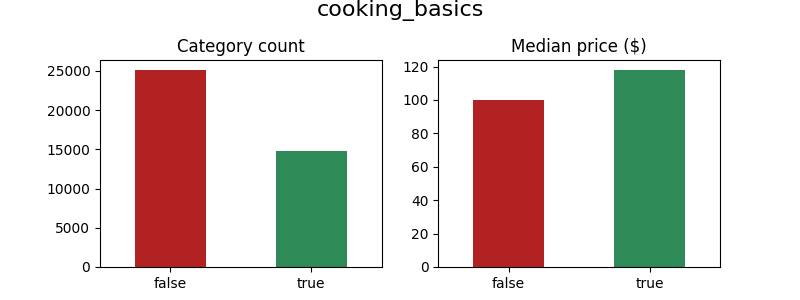
\includegraphics[width=\linewidth]{figures/amenities/group1/cooking_basics.png}
    %\caption{Caption 2}
    \label{fig:private-entrance-and-cooking-basics}
\end{figure}


% Amenity Group 2
\begin{figure}[H]
\centering
\caption{TV and Internet}
    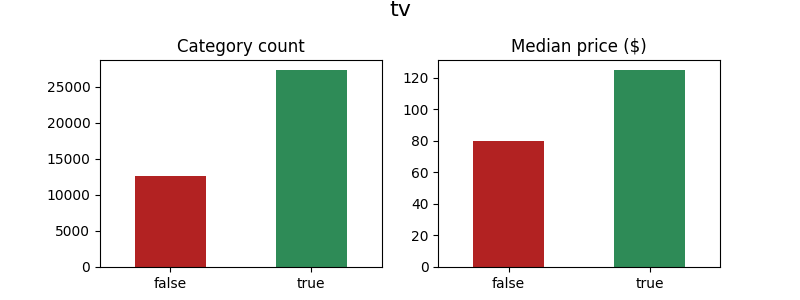
\includegraphics[width=\linewidth]{figures/amenities/group2/tv.png}
    %\caption{Caption 1}
    \vspace{0.5cm}
    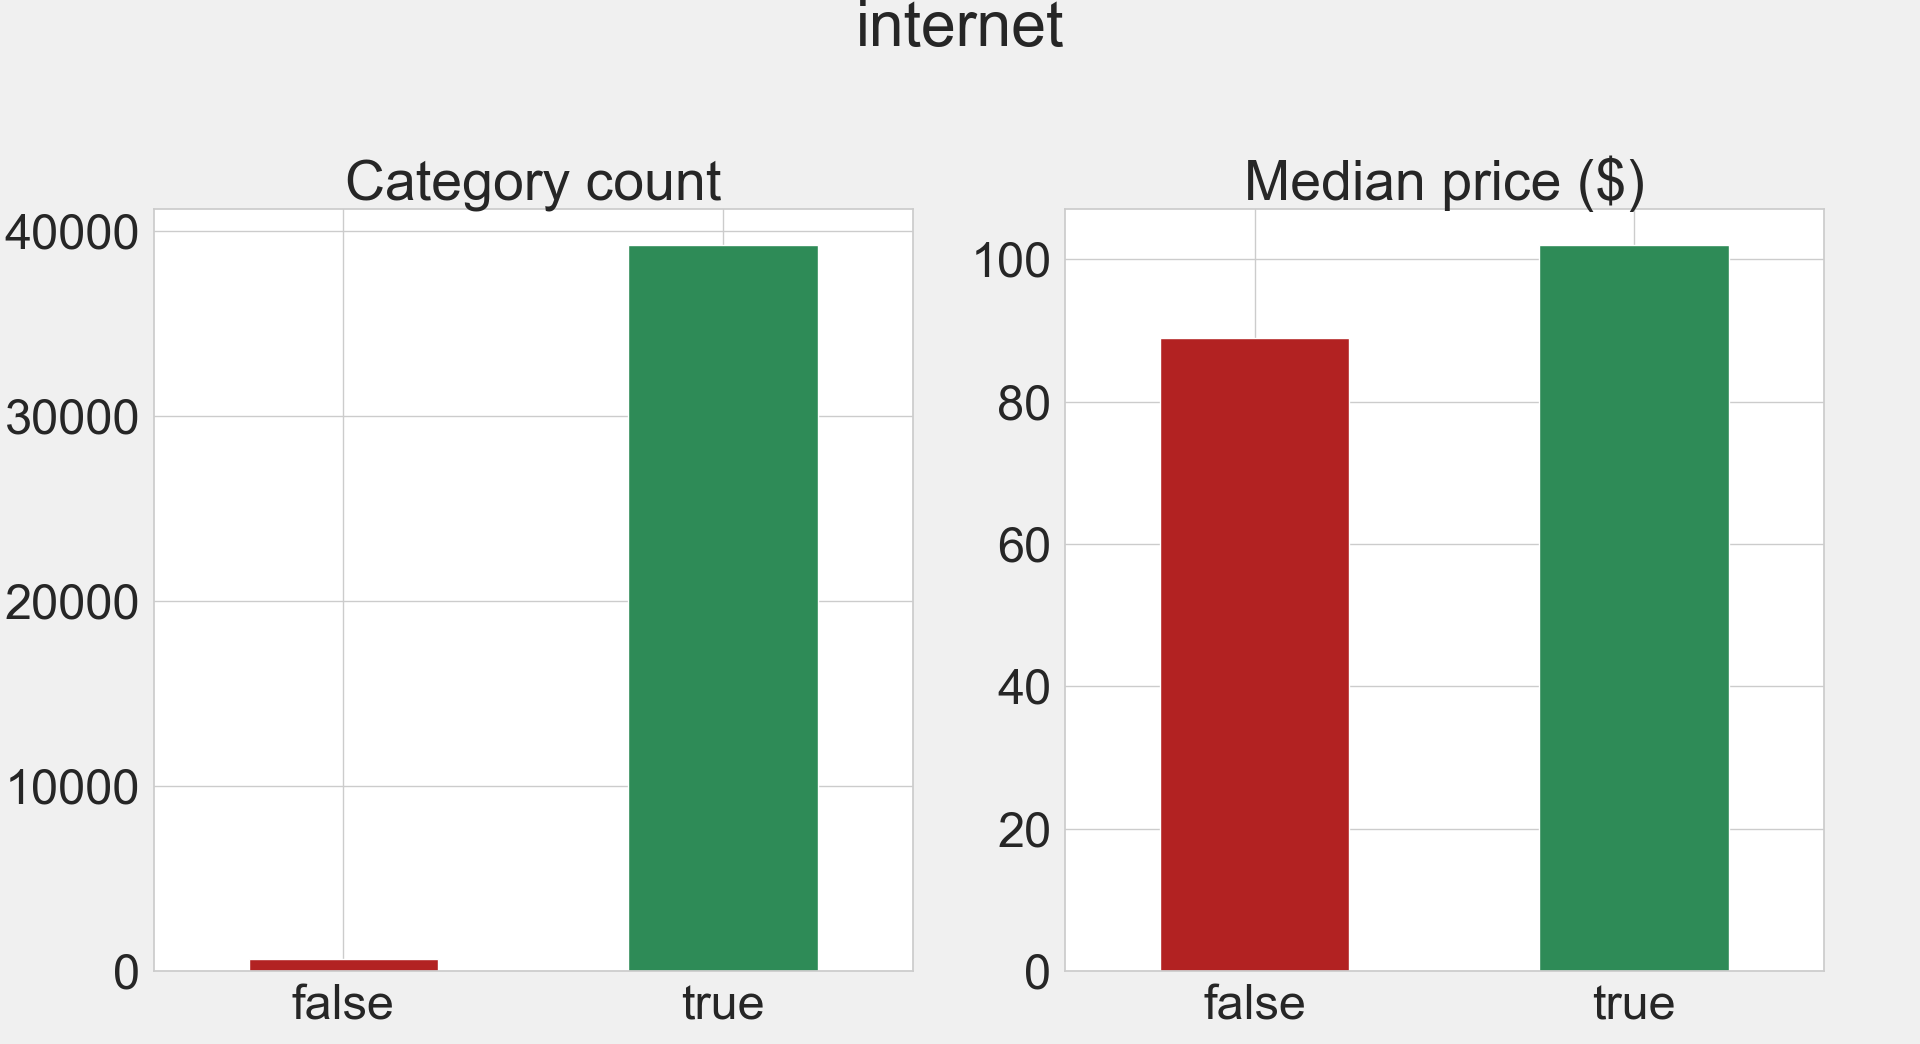
\includegraphics[width=\linewidth]{figures/amenities/group2/internet.png}
    %\caption{Caption 2}
    \label{fig:tv-and-internet}
\end{figure}

\begin{figure}[H]
\centering
    \caption{Air Conditioner}
    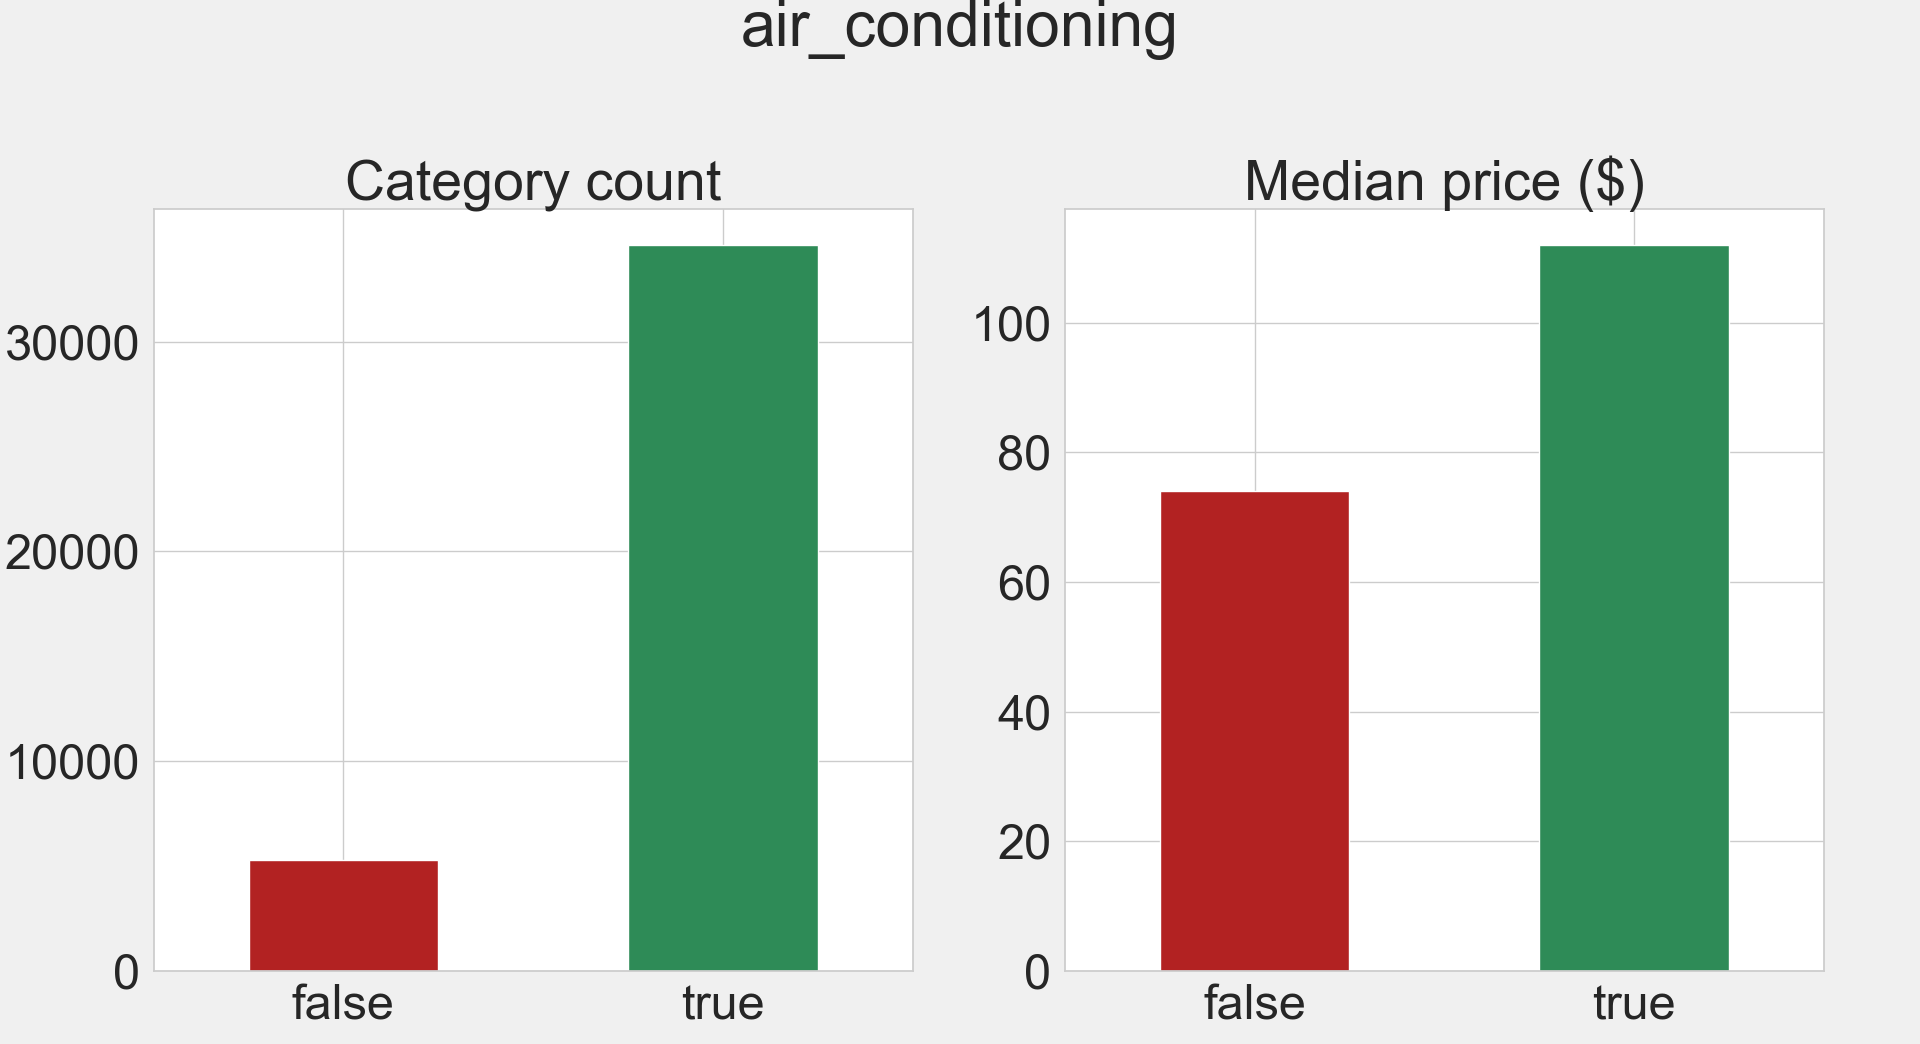
\includegraphics[width=\linewidth]{figures/amenities/group2/air_conditioning.png}
    \label{fig:air-conditioner}
\end{figure}

% Amenity Group 3
\begin{figure}[H]
\centering
    \caption{Parking and Host Greeting}
    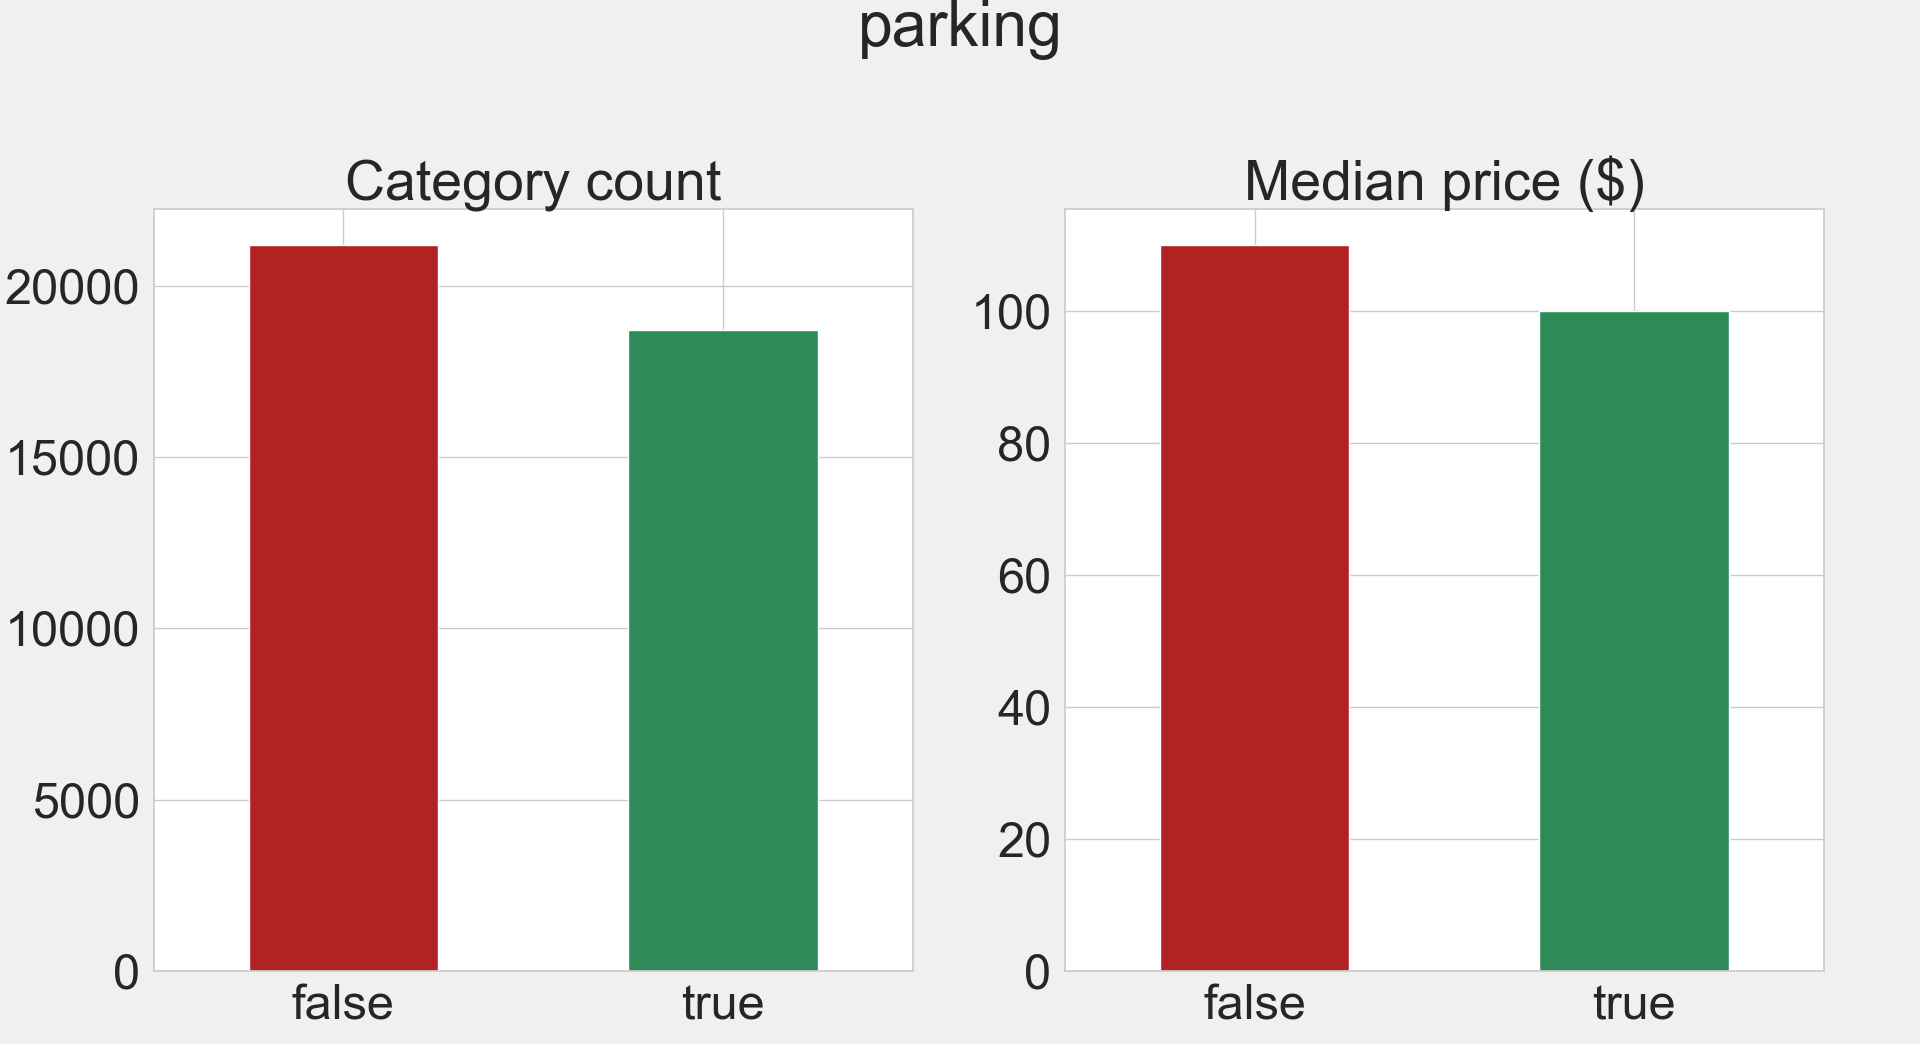
\includegraphics[width=\linewidth]{figures/amenities/group3/parking.png}
    \vspace{0.5cm}
    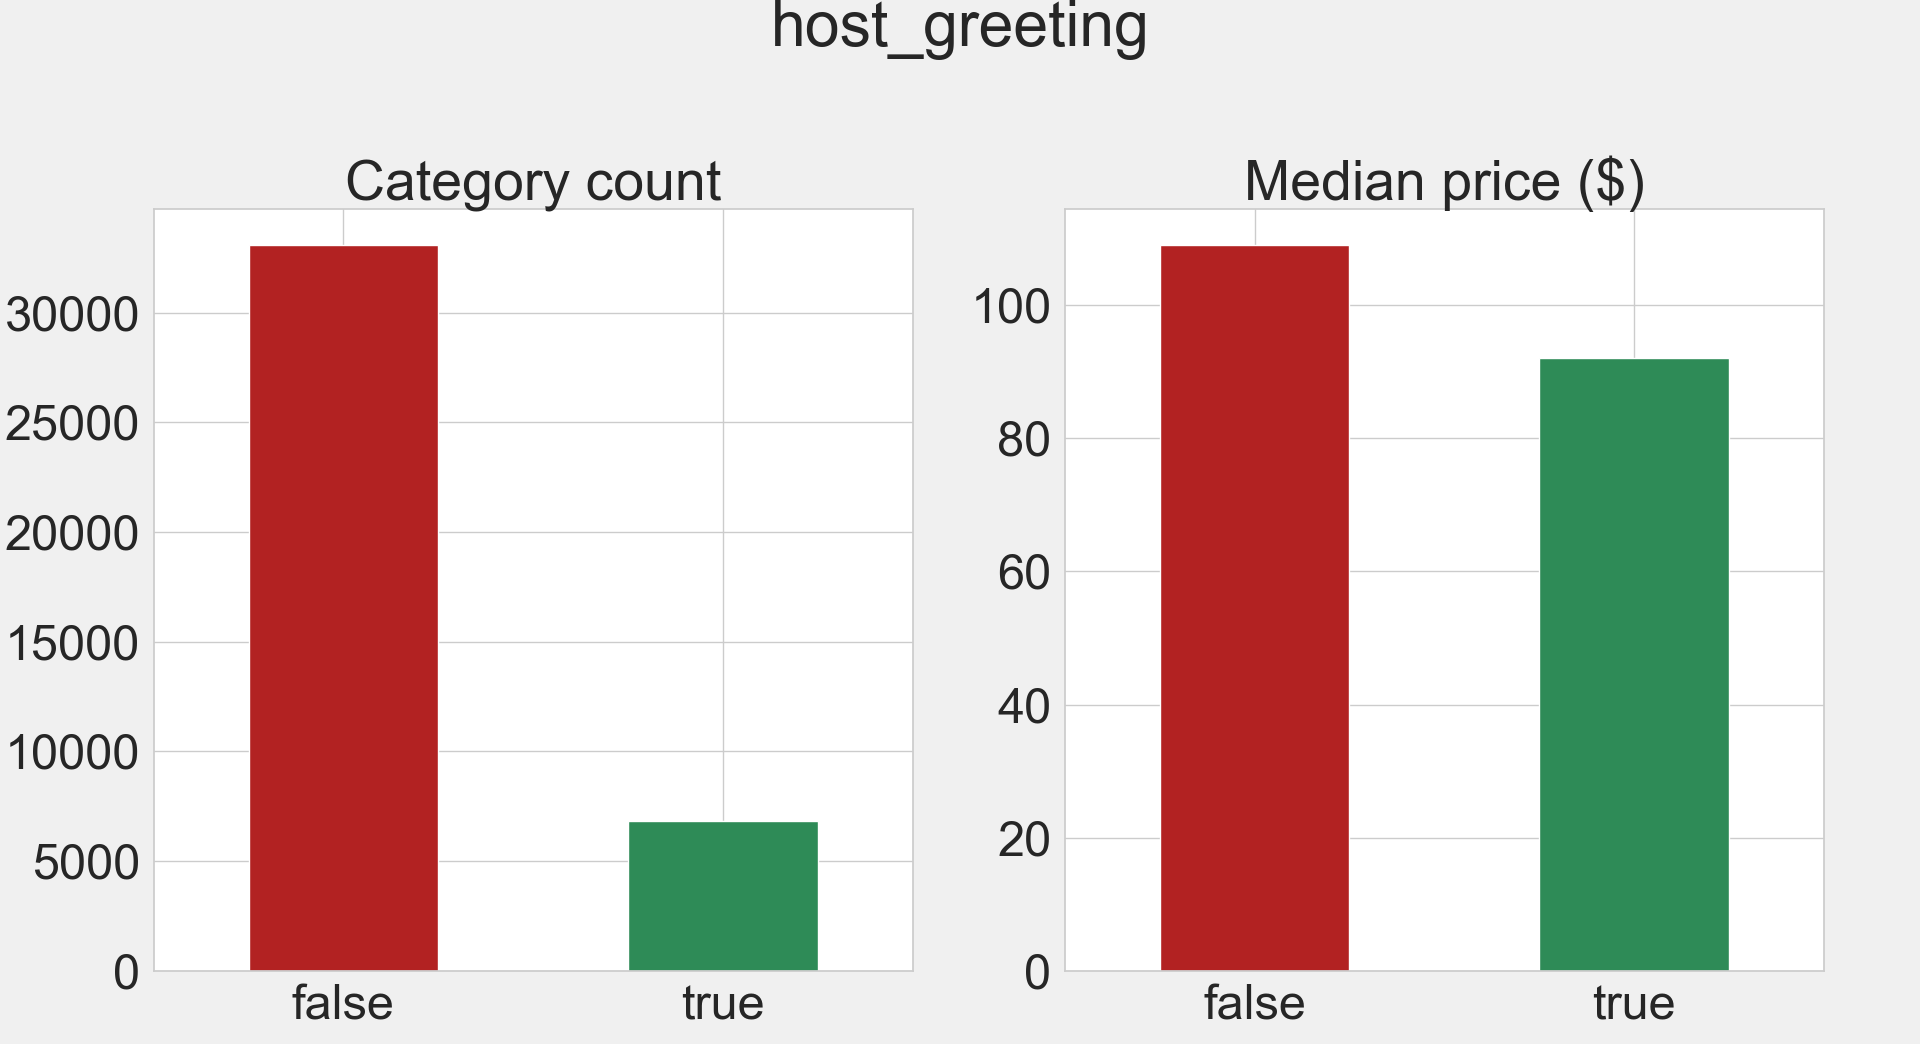
\includegraphics[width=\linewidth]{figures/amenities/group3/host_greetings.png}
    \label{fig:parking-and-host-greeting}
\end{figure}


\begin{figure}[H] \centering
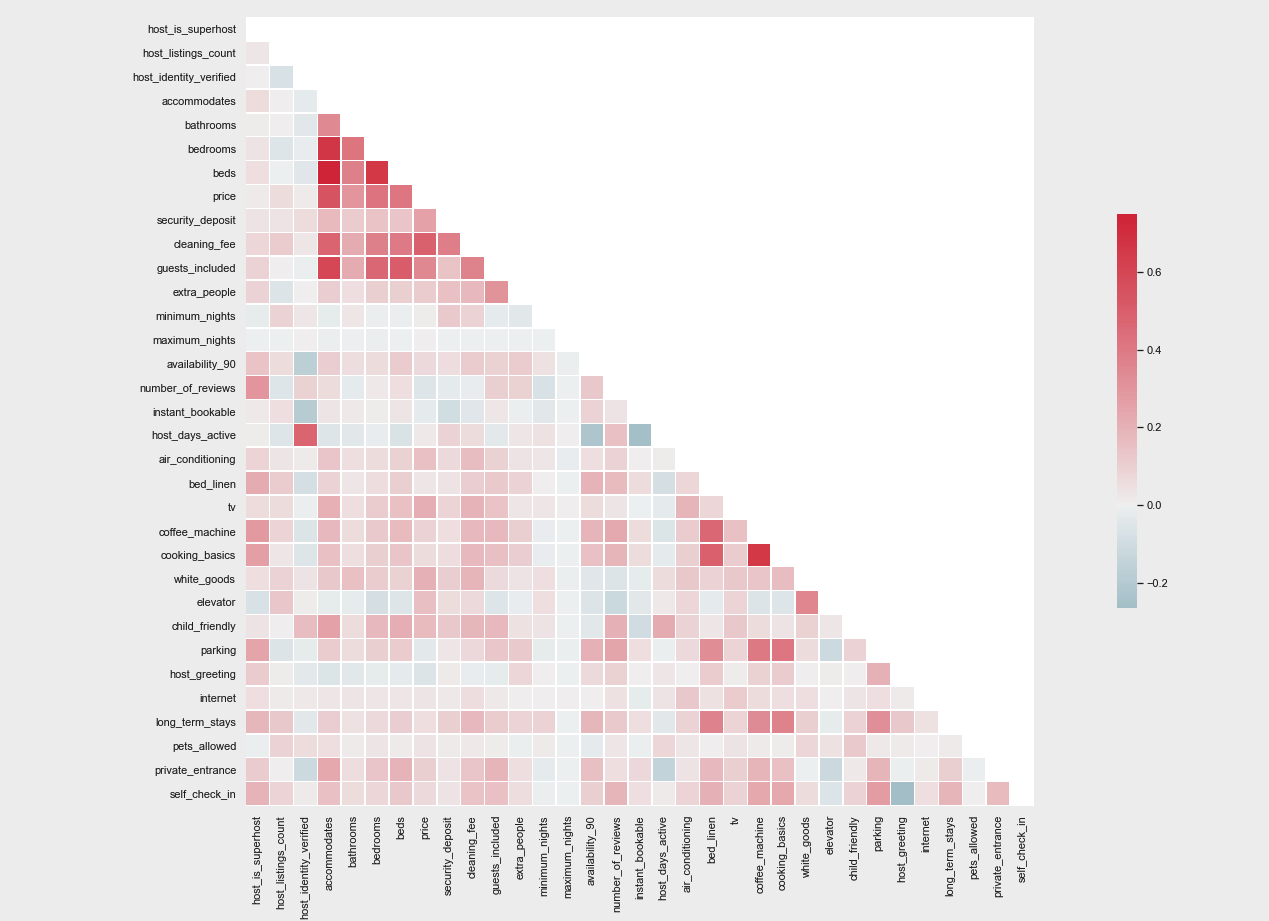
\includegraphics[width=\textwidth,keepaspectratio]{correlation-matrix.png}
\caption{Correlation Matrix}
\label{fig:correlation-matrix}
\end{figure}

\begin{figure}[H] \centering
\caption{Histogram of Feature Distribution}
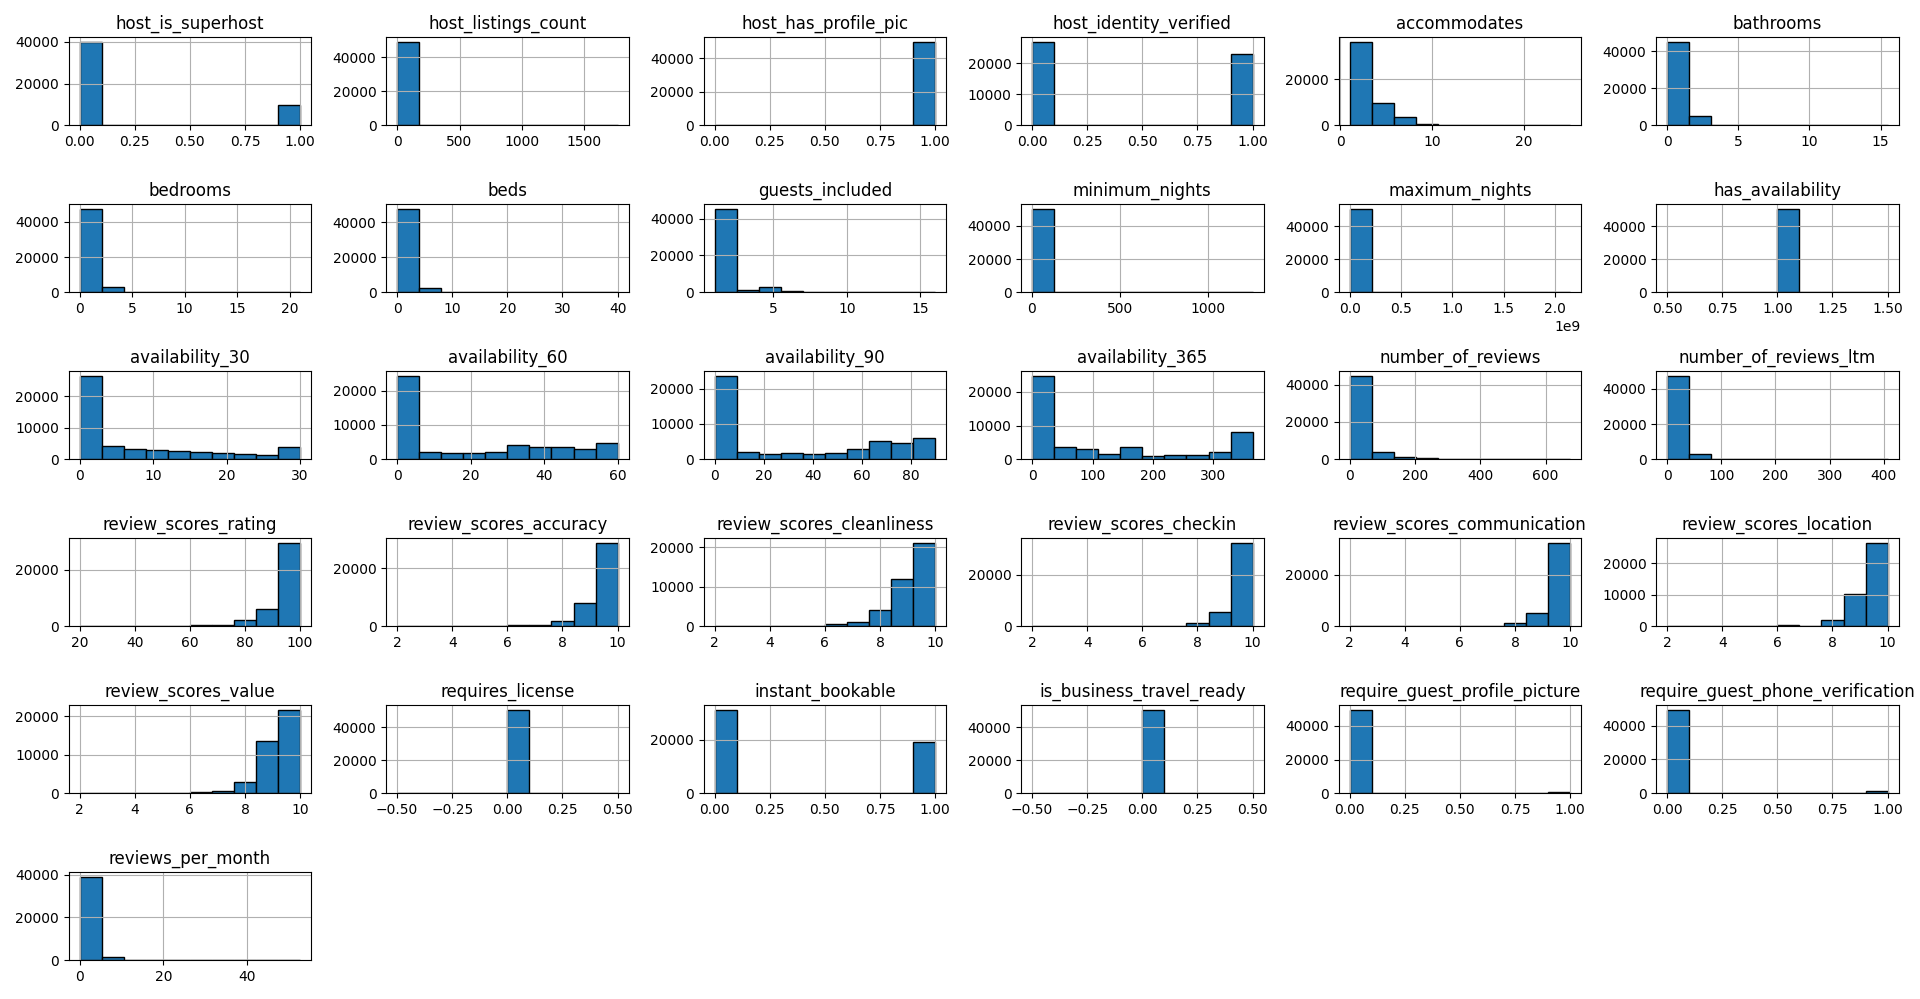
\includegraphics[width=\textwidth]{Figure_0_histogram.png}
\label{fig:histogram-feature-distribution}
\end{figure}

% from pre_processing.py
%Other than availability_90 and host_days_active, the remaining numerical
%features are all postively skewed and could benefit from log transformation.
\begin{figure}[H] \centering
\caption{Histogram of Numerical Feature Distribution Before Log Transform }
\includegraphics[width=\textwidth]{before-log.png}
\label{fig:histogram-before-transform}
\end{figure}

% from pre_processing.py
\begin{figure}[H] \centering
\caption{Histogram of Numerical Feature Distribution After Log Transform }
\includegraphics[width=\textwidth]{after-log.png}
\label{fig:histogram-after-transform}
\end{figure}




\clearpage
	\fancyhf{}
	\rhead{\thepage}
	\lhead{\textbf{ \nouppercase{\leftmark}} }
\phantomsection
\addcontentsline{toc}{chapter}{Bibliography}
%\pagenumbering{roman}
%\bibliographystyle{chicago}
%\bibliography{bib_file}
\printbibliography

%\clearpage
%\renewcommand{\thefigure}{A\arabic{figure}}
%\renewcommand{\thetable}{A\arabic{table}}
%\setcounter{figure}{0}
%\setcounter{table}{0}
%\section*{Appendix}
%\label{appendix}
\end{onehalfspace}
\end{document}
